%pour la mise en page
\documentclass[a4paper,10pt]{report}
\usepackage[utf8]{inputenc}
\usepackage[Conny]{fncychap}
%Sonny Lenny Glenn Conny Rejne et Bjarne

%pour les maths
\usepackage{graphicx}
\usepackage{amsmath}
\usepackage{indentfirst}
\usepackage{amssymb}

%pour les figures
\usepackage{float}

%pour les algorithmes
\usepackage{algorithm}
\usepackage{algorithmic}
%francisation des algorithmes
\renewcommand{\algorithmicrequire} {\textbf{\textsc{Initialisation}}}
\renewcommand{\algorithmicensure}  {\textbf{\textsc{Sorties:}}}
\renewcommand{\algorithmicand}      {\textbf{et}}
\renewcommand{\algorithmicwhile}   {\textbf{Tant que}}
\renewcommand{\algorithmicdo}      {\textbf{faire}}
\renewcommand{\algorithmicendwhile}{\textbf{fin tant que}}
\renewcommand{\algorithmicend}     {\textbf{fin}}
\renewcommand{\algorithmicif}      {\textbf{Si}}
\renewcommand{\algorithmicendif}   {\textbf{fin si}}
\renewcommand{\algorithmicelse}    {\textbf{Sinon}}
\renewcommand{\algorithmicthen}    {\textbf{alors}}
\renewcommand{\algorithmicfor}     {\textbf{Pour}}
\renewcommand{\algorithmicforall}  {\textbf{Pour tout}}
\renewcommand{\algorithmicendfor}  {\textbf{fin pour}}
\renewcommand{\algorithmicloop}    {\textbf{Boucler}}
\renewcommand{\algorithmicendloop} {\textbf{fin boucle}}
\renewcommand{\algorithmicrepeat}  {\textbf{Répéter}}
\renewcommand{\algorithmicuntil}   {\textbf{Jusqu'à}}

\usepackage{color}
\definecolor{gray}{rgb}{0.5, 0.5, 0.5}
\definecolor{lightgray}{rgb}{0.96, 0.96, 0.96}
\definecolor{orange}{rgb}{1.0, 0.5, 0.0}
\definecolor{blue}{rgb}{0.0, 0.0, 1.0}
\definecolor{red}{rgb}{0.8, 0.0, 0.0}

%pour les programmes
\usepackage{listings}
	\lstset{
		language=scilab,
		basicstyle=\small,
		keywordstyle=\bf \color{orange},
		identifierstyle=\color{blue},
		commentstyle=\color[gray]{0.5},
		stringstyle=\color{red},
		showstringspaces=false,
		numbers=left,
		numberstyle=\tiny \bf \color{gray},
		numbersep=10pt,
		numberfirstline=true,
		backgroundcolor=\color{lightgray},
}

\usepackage[top=3cm, bottom=3cm, left=3cm, right=3cm]{geometry}

\renewcommand{\chaptername}{Chapitre}
\renewcommand{\contentsname}{Table des matières}
\renewcommand{\listfigurename}{Table des Figures}
\renewcommand{\listtablename}{Table des Codes}
\renewcommand{\tablename}{Code}

\usepackage{eso-pic}
	\newcommand\BackgroundPic{%
		\put(0,0){
			\parbox[b][\paperheight]{\paperwidth}{%
			\vfill
			\centering
			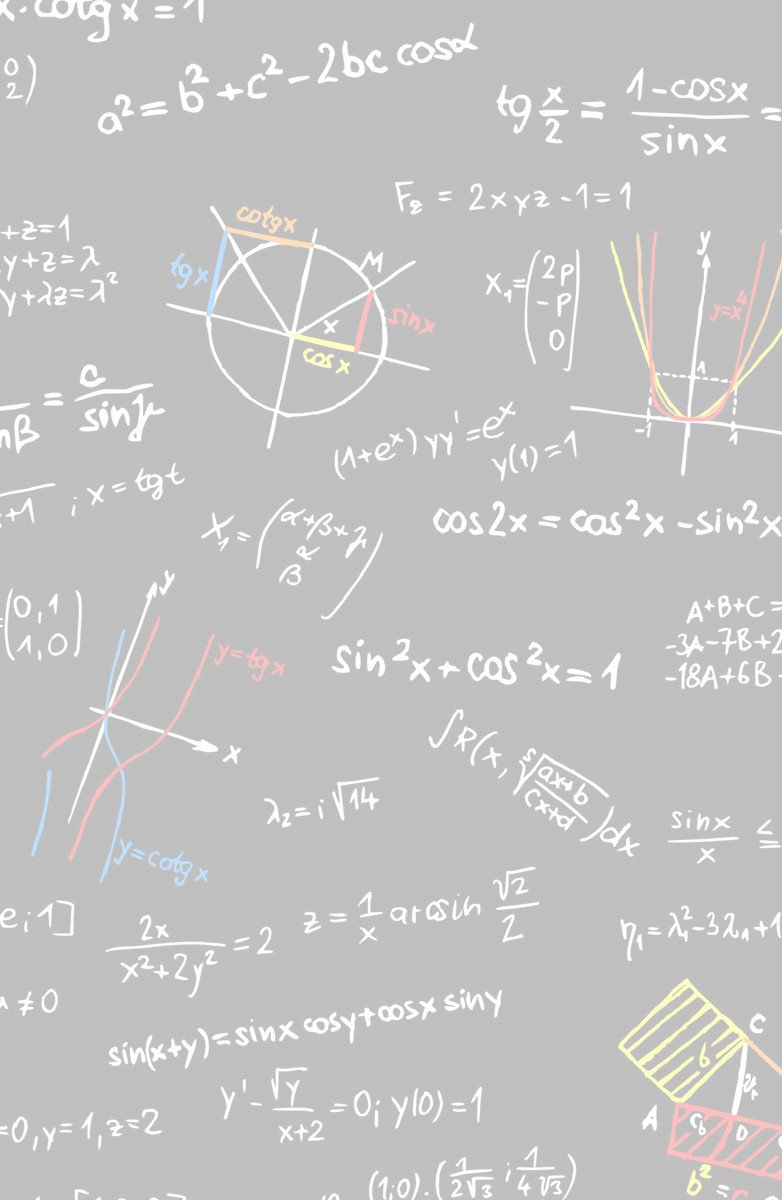
\includegraphics[width=\paperwidth,height=\paperheight]{mathtimes.png}%
			\vfill
		}}}

\usepackage{fancyhdr}
\pagestyle{fancy}
\renewcommand\headrulewidth{1pt}
\fancyhead[L]{Cahier d'intégration MT94}
\fancyhead[R]{\leftmark}
\renewcommand\footrulewidth{1pt}
\fancyfoot[L]{UTC}
\fancyfoot[C]{\thepage}
\fancyfoot[R]{Marlow Justine}

\makeatletter
\let\ps@plain=\ps@fancy
\makeatother

\begin{document}
\AddToShipoutPicture*{\BackgroundPic}
\title{Cahier d'intégration MT94}
\author{Marlow Justine}
\date{}
\maketitle

\addcontentsline{toc}{chapter}{Table des matières}
\tableofcontents
\newpage
\addcontentsline{toc}{chapter}{Table des figures}
\listoffigures
\newpage
\addcontentsline{toc}{chapter}{Table des codes}
\listoftables

\newpage
\addcontentsline{toc}{chapter}{Résumé}
\chapter*{Résumé}
\markboth{RESUME}{}
Blabla résumé, MT94

\chapter{Problèmes non linéaires I}

\section{Introduction}
\indent Les problèmes non linéaires constituent un ensemble de problèmes mathématiques qui sont, pour la plupart, insolubles de manière analytique. Ces problèmes peuvent en effet se ramener à la recherche des solutions de $f(x)=0$. Or la recherche de racines devient problématique lorsque le degré du polynôme $f$ augmente, impossible de déterminer des solutions analytiquement pour un degré supérieur ou égal à 4. Il existe donc des méthodes numériques afin d'approcher ces solutions. Nous allons étudier quelques une de ces méthodes au sein de ce chapitre.\\ \\
\indent Les trois premières méthodes étudiées, à savoir \textit{la dichotomie}, \textit{la méthode des points fixes} et \textit{la méthode de Newton}, concernent les problèmes à une inconnue : $f : \mathbb{R} \longrightarrow \mathbb{R}$. Nous verrons également l'application de \textit{la méthode de la sécante}, qui se trouve être une méthode dérivée de \textit{la méthode de Newton}. La dernière méthode étudiée, qui est également \textit{la méthode de Newton}, permet de traiter des problèmes à $n$ ($n>1$) inconnues : $f : \mathbb{R}^n \longrightarrow \mathbb{R}^n$.\\ \\
\indent Pour chacune de ces méthodes, nous étudierons tout d'abord leur aspect théorique avant de les appliquer dans \textit{Scilab}. Cette application suivra toujours la même démarche :
\begin{itemize}
\item Résoudre le problème par exécution du code
\item Tracer la courbe de l'erreur en fonction de l'itération avec la commande : \begin{verbatim} --> plot(erreur,'o')
\end{verbatim}
\item Tracer la courbe de régression linéaire avec la commande : \begin{verbatim}
--> plot(log(erreur(1:k-1))',log(erreur(2:k))')
\end{verbatim} et connaître son coefficient directeur avec la commande : \begin{verbatim}
--> reglin(log(erreur(1:k-1))',log(erreur(2:k))')
\end{verbatim}
\end{itemize}

\newpage
\section{La dichotomie ou bissection}
\subsubsection{Théorie}
La dichotomie est une méthode de résolution numérique répandue et enseignée dés le lycée. Son principal avantage est qu'elle ne nécessite qu'une seule hypothèse : la continuité de $f$ sur un intervalle $I\subset \mathbb{R}$.\\
\indent La fonction $f : \mathbb{R} \longrightarrow \mathbb{R}$ est donc continue sur un intervalle $I$. On va par ailleurs supposer que l'on travaille sur un intervalle $[a,b]\subset I$ tel que $f(a)f(b)<0$. La continuité de $f$ permet d'appliquer le théorème des valeurs intermédiaires : il existe $x^{*}\in[a,b]$ tel que $f(x^{*})=0$.\\
\indent Le principe de l'algorithme est alors le suivant : on définit :\\ $(a_{n})_{,\ n \geq 0},\ (b_{n})_{,\ n \geq 0},\ a_{0}=a,\ b_{0}=0,\ (x_{n})_{, n \geq 0},\ x_{n} = \frac{a_{n}+b_{n}}{2}, a_{n+1}$ et $b_{n+1}$ par:

\begin{algorithm}
\begin{algorithmic}
\WHILE{$|f(x_n)|>\varepsilon$ ($\varepsilon$ désigne la précision recherchée)}
\IF{$f(a_{n})f(b_{n})>0$}
\STATE $a_{n+1}=x_{n}$
\ELSE
\STATE $b_{n+1}=x_{n}$
\ENDIF
\ENDWHILE
\end{algorithmic}
\end{algorithm}

\indent Pour juger de l'efficacité de cette méthode, on s'intéresse à la convergence de la suite. Par construction, on a $(b_{n} - a_{n})=(\frac{1}{2}){n}(b_{0} - a_{0})$.\\
Ainsi $|x_{n} - x^{*}|\leq\frac{1}{2}(b_{n} - a_{n})$ donc $|x_{n} - x^{*}|\leq\frac{1}{2}^{n+1}(b_{0} - a_{0})$.

\subsubsection{Application}
Pour cette application, on étudie $f : \mathbb{R} \longrightarrow \mathbb{R}$ définie telle que $f(x)=x^2-2$. On connaît évidemment la solution de cette équation, il s'agit de $\pm\sqrt{2}$. On choisit donc un intervalle $[a,b]$ qui encadre seulement une solution, $\sqrt{2}$, on prendra ici $[a,b]=[1,2]$. On implémente donc dans \textit{Scilab} le code \ref{dichotomie}.
\begin{table}[H]
\label{dichotomie}
\caption{Dichotomie}
\begin{tabular}{l}
\lstinputlisting[language=scilab]{dichotomie.sce}\\
\end{tabular}
\end{table}

On trace l'évolution de l'erreur en fonction de l'itération (figure \ref{graph_dicho}).
\begin{center}
\begin{figure}[H]
\caption{Erreur en fonction de l'itération}
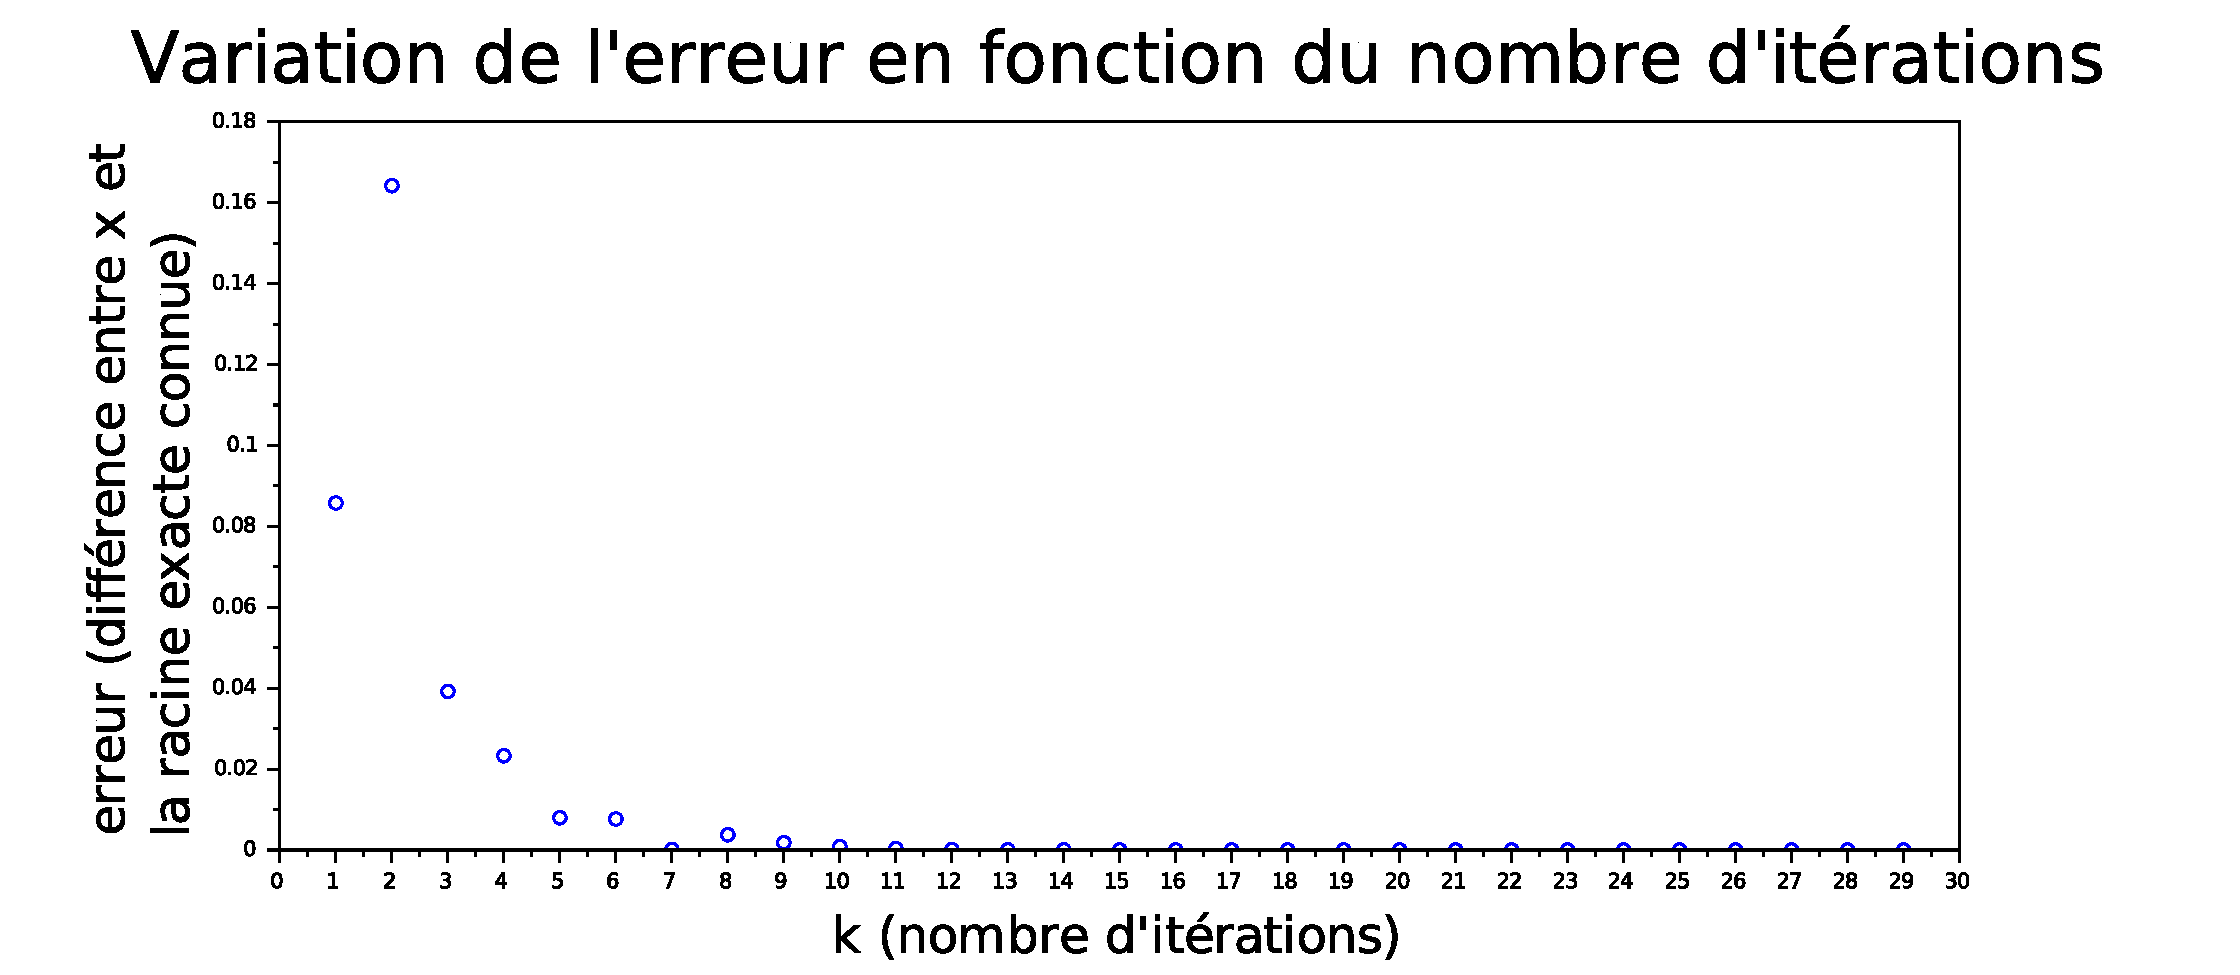
\includegraphics[width=\textwidth]{graphdicho.pdf}
\label{graph_dicho}
\end{figure}
\end{center}

Puis on s'intéresse à l'évolution de l'erreur relative (figure \ref{erreur_dicho}).
\begin{center}
\begin{figure}[H]
\caption{Diminution relative de l'erreur en fonction de l'itération}
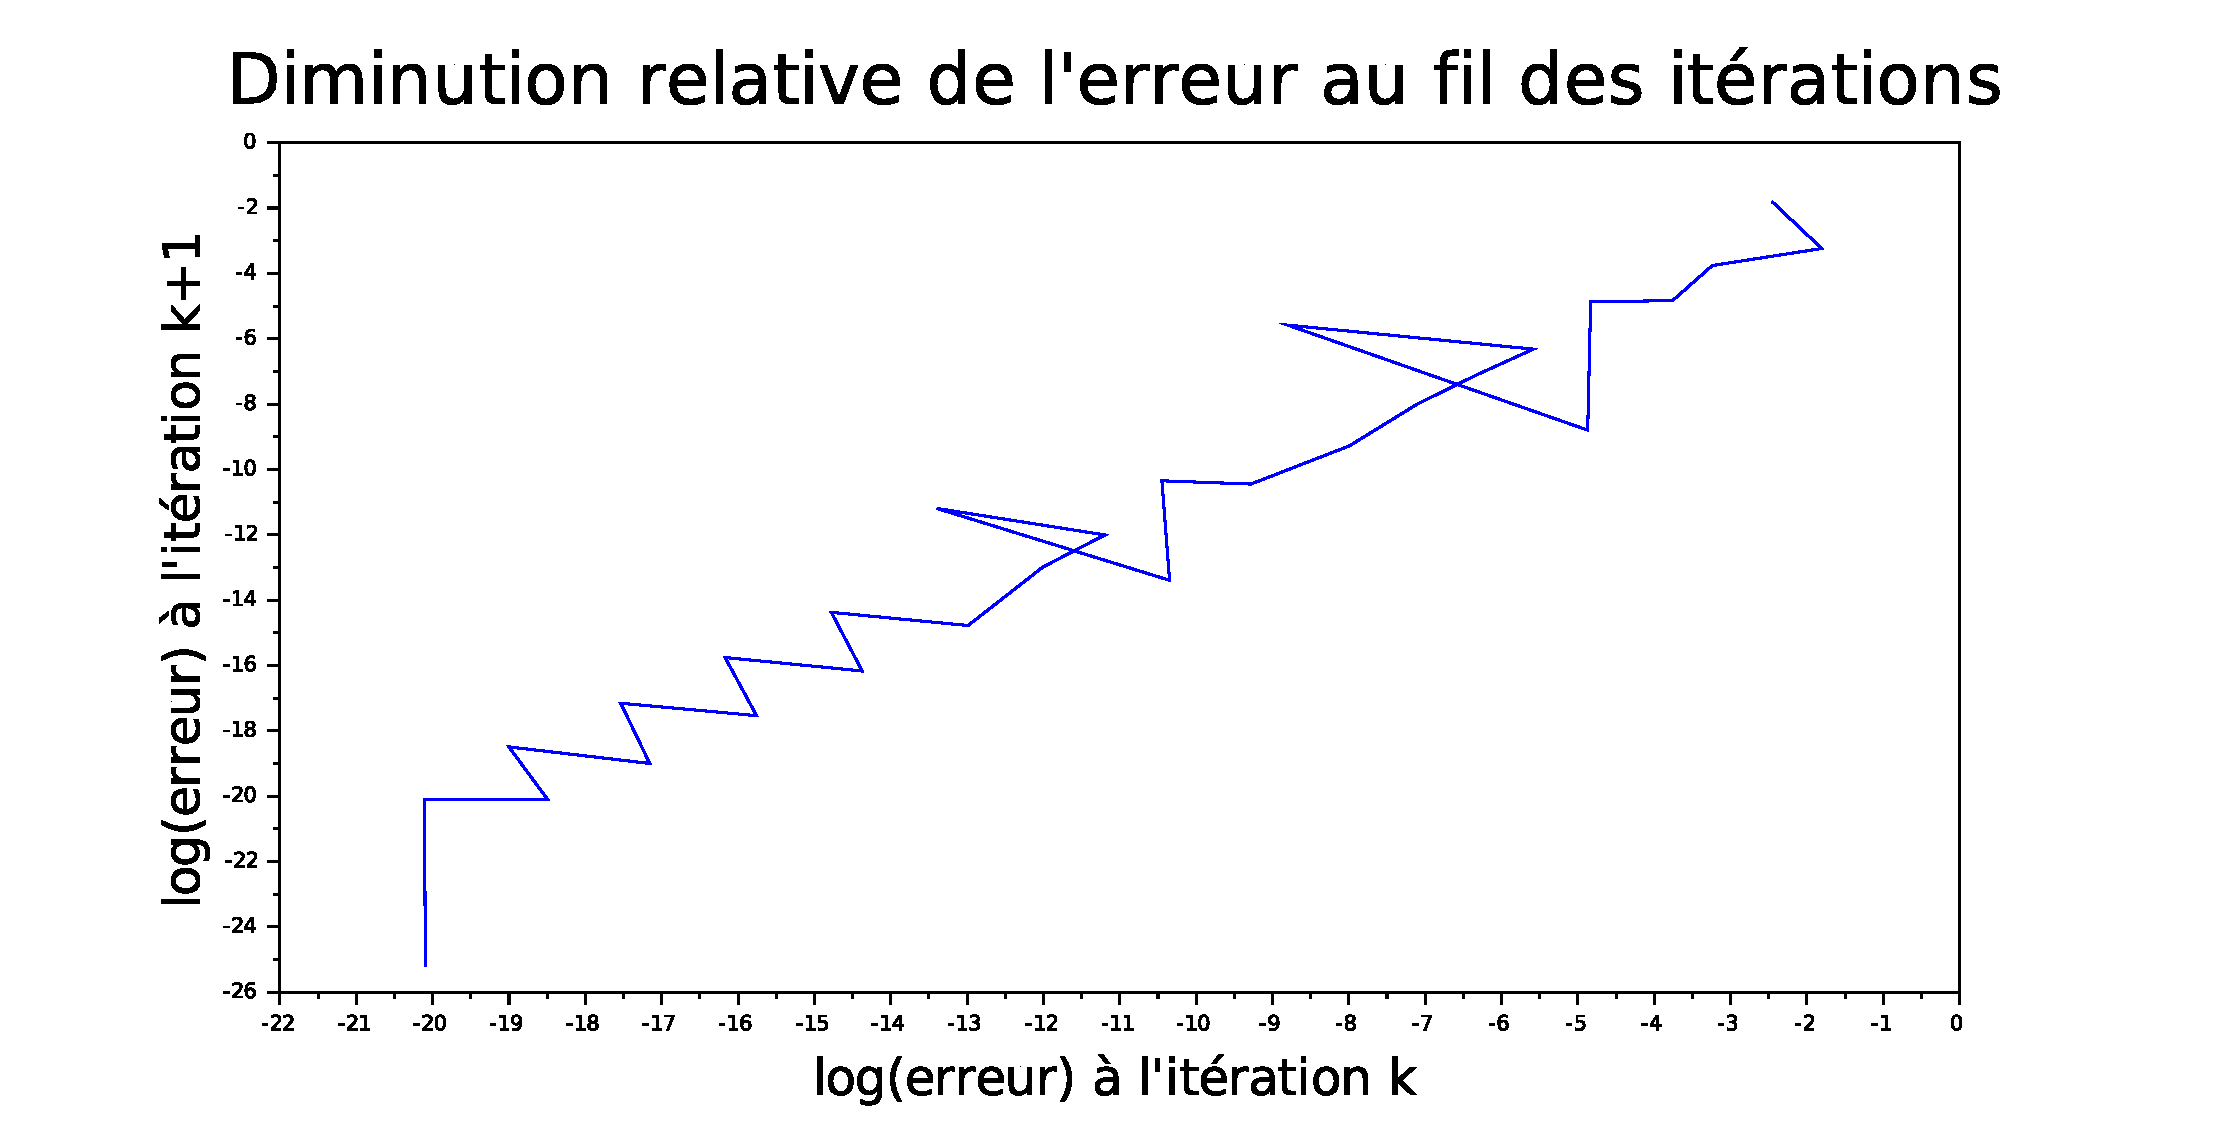
\includegraphics[width=\textwidth]{graphdicho_reg.pdf}
\label{erreur_dicho}
\end{figure}
\end{center}

La solution est donc approchée en 29 itérations. Une remarque toute particulière pour la dichotomie : l'erreur n'est pas réduit de manière uniforme au fil des itérations (comme le montre la figure \ref{erreur_dicho}). Si on linéarise cette courbe (figure \ref{erreur_dicho}) grâce à \textit{Scilab}, on obtient un coefficient proche de 1 (environ 1,0188), il s'agit effectivement d'une convergence linéaire, ou d'ordre 1.

\newpage
\section{La méthode de point fixe}
\subsubsection{Théorie}
Cette méthode, également répandue, nécessite toutefois plus d'hypothèses que la dichotomie, en effet il est nécessaire que $f$ soit une fonction dérivable.\\
\indent L'idée de la méthode est de rechercher une fonction $g : \mathbb{R} \longrightarrow \mathbb{R}$ telle que $f(x)=0 \Leftrightarrow g(x)=x$. Cette fonction $g$ (supposée dérivable) admet ainsi un point fixe, notons le $x^*$ tel que $|g'(x^*)|<1$. Alors, en appliquant le théorème des accroissements finis, il existe $[a,b]$ tel que $x^*\in[a,b]$ et la suite :\\
$
\left\lbrace
\begin{array}{l}
x_0\in[a,b]\\
x_{n+1}=g(x_n), n\geq0
\end{array}\right.
$ converge vers $x^*$ (la démonstration est admise ici, détaillée en MT90).\\ \\
\indent Comme avec la dichotomie, s'intéresser à la convergence de la suite nous indique sur l'efficacité de la méthode. Si $g'(x^*)\neq0$ alors $\frac{|x_{n+1}-x^*|}{|x_{n}-x^*|}<k$ avec $0<k<1$. \\
\noindent Par récurrence, $|x_{n+1}-x^*|<k^n|x_{0}-x^*|$.

\subsubsection{Application}
A nouveau, on étudie $f : \mathbb{R} \longrightarrow \mathbb{R}$ définie telle que $f(x)=x^2-2$. Comme précédemment, on choisit l'intervalle $[a,b]=[1,2]$, et on choisit ici $x_0=\frac{3}{2}$ (on se place au milieu de l'intervalle d'étude). On implémente donc dans \textit{Scilab} le code \ref{code_pointfixe}.

\begin{table}[H]
\caption{Point fixe}
\begin{tabular}{l}
\lstinputlisting[language=scilab]{pointfixe.sce}
\label{code_pointfixe}
\end{tabular}
\end{table}

\newpage
On trace l'évolution de l'erreur en fonction de l'itération (figure \ref{graph_pointfixe}).
\begin{figure}[H]
\centering
\caption{Erreur en fonction de l'itération}
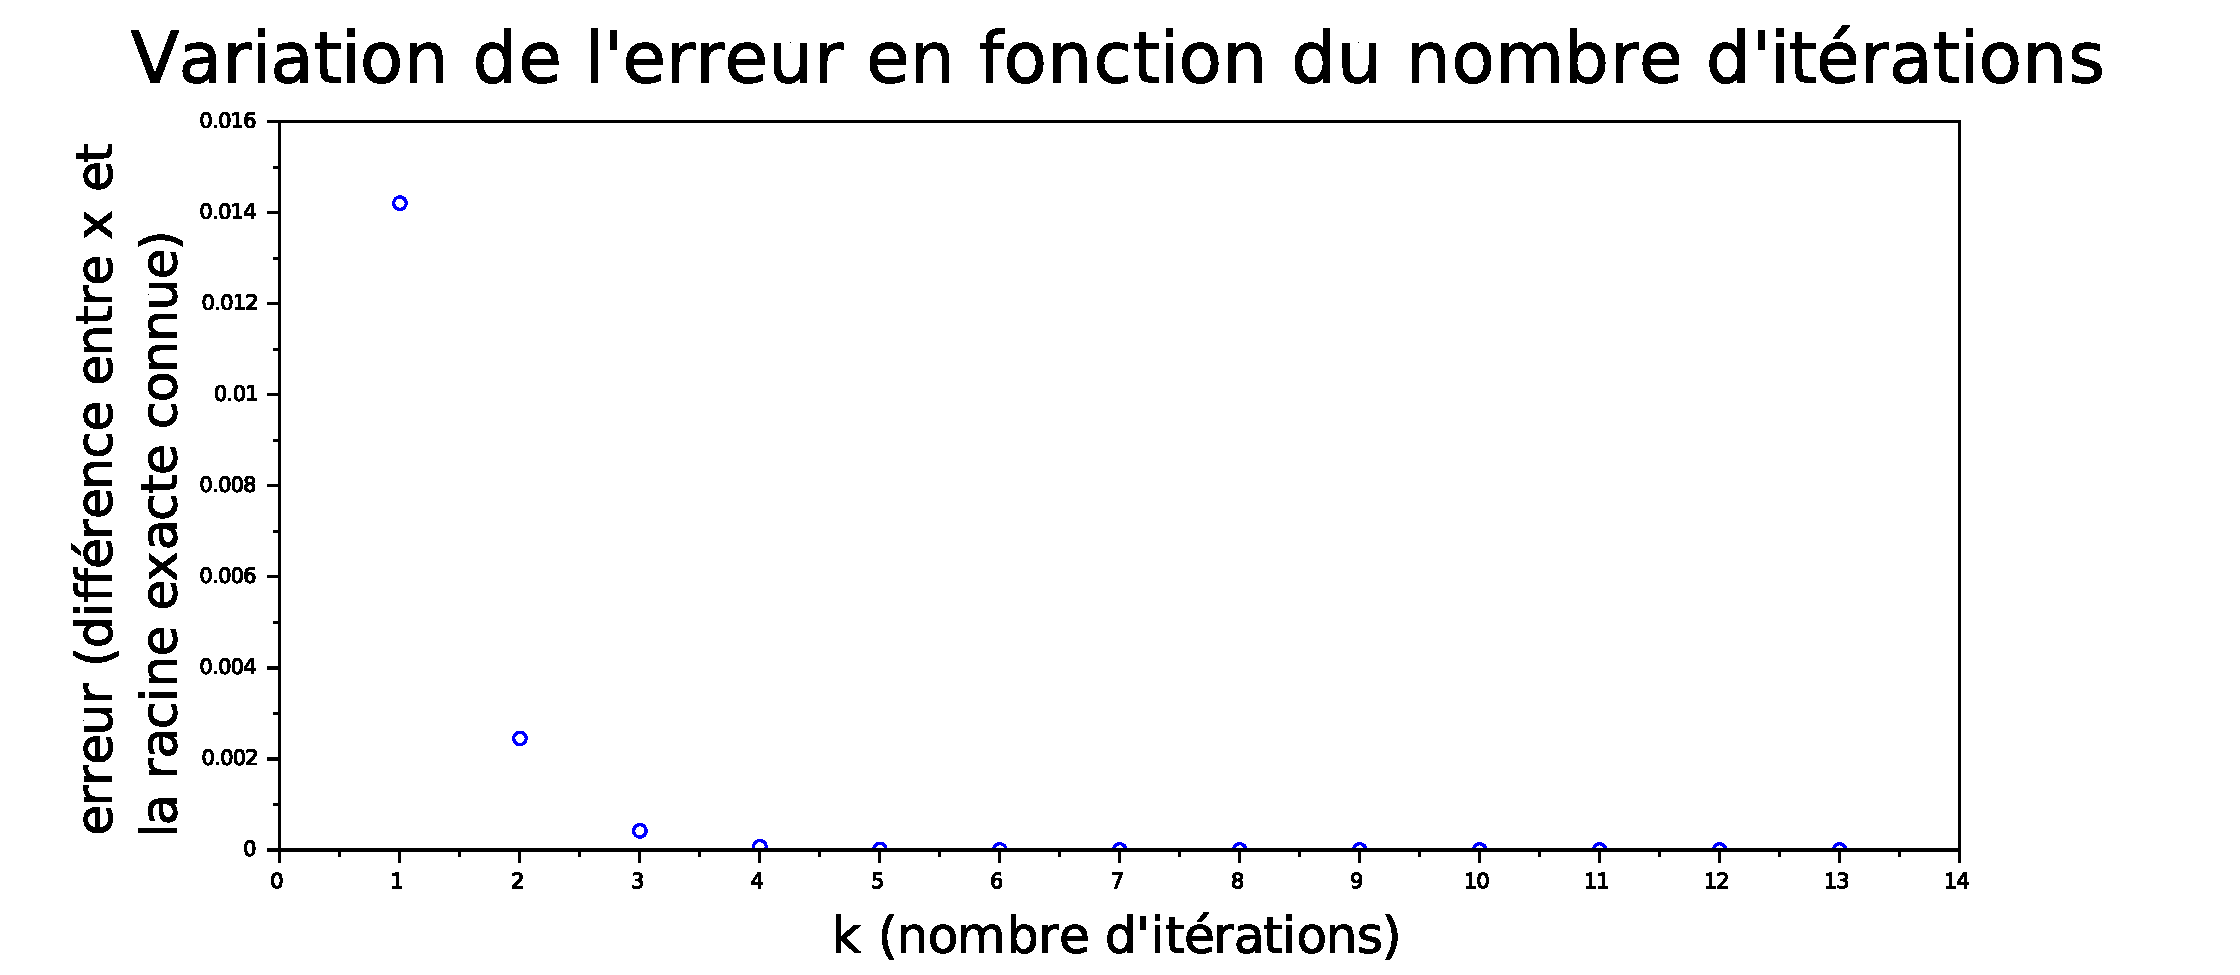
\includegraphics[width=\textwidth]{graphpointfixe.pdf}
\label{graph_pointfixe}
\end{figure}

Puis on s'intéresse à l'évolution de l'erreur relative (figure \ref{erreur_pointfixe}).
\begin{center}
\begin{figure}[H]
\caption{Diminution relative de l'erreur en fonction de l'itération}
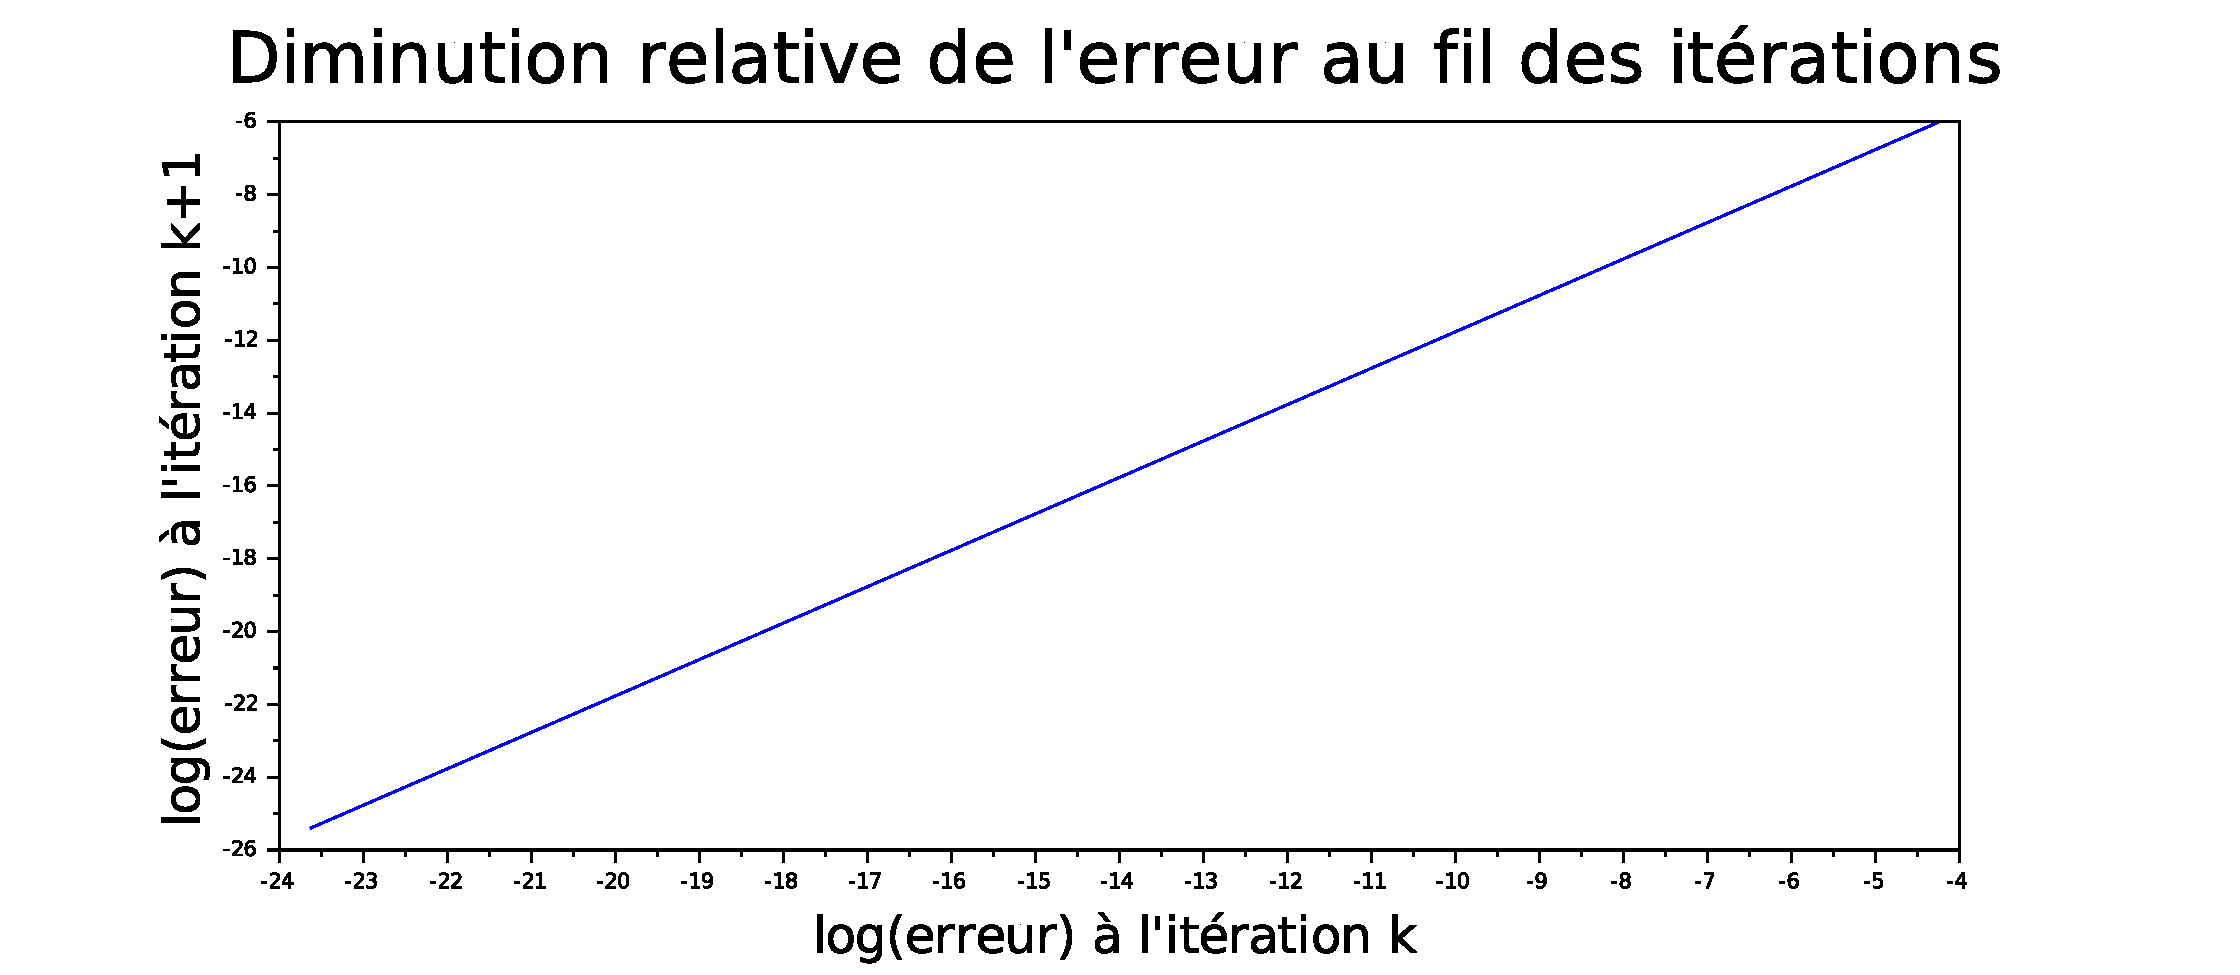
\includegraphics[width=\textwidth]{graphpointfixe_reg.pdf}
\label{erreur_pointfixe}
\end{figure}
\end{center}

La solution est donc approchée en 13 itérations. Si on linéarise cette courbe (figure \ref{erreur_pointfixe}) grâce à \textit{Scilab}, on obtient un coefficient très proche de 1 (environ 1,0001), effectivement, il s'agit à nouveau d'une convergence d'ordre 1.

\newpage
\section{La méthode de Newton appliquée à $n=1$}
\subsubsection{Théorie}
La méthode de Newton nécessite encore plus d'hypothèses que les deux méthodes que nous venons d'étudier. En effet, on suppose ici que la fonction $f$ est deux fois continûment dérivable. On écrit ensuite le développement de Taylor Lagrange sur $f$ : soit $x_{0}\in\mathbb{R}$, il existe $\theta\in]0,1[$,\\
$f(x_0+h)=f(x_0)+f'(x_0)h + \frac{h^2}{2}f''(x_0+\theta h)$\\
si on pose $x=x_0+h$, le développement devient :\\
$f(x)=f(x_0)+f'(x_0)(x-x_0) + \frac{{x-x_0}^2}{2}f''(x_0+\theta (x-x_0))$\\
On effectue l'approximation affine de $f(x)$ : $T_{x_0}(x)=f(x_0)+f'(x_0)(x-x_0)$\\
et on définit $x_1$ par $T_{x_0}(x_1)=0 \Leftrightarrow f(x_0)+f'(x_0)(x_1-x_0)=0$\\
si $f'(x_0)\neq0$ alors $x_1=x_0 - \frac{f(x_0)}{f'(x_0)}$.\\
Ainsi, graphiquement, la méthode de Newton consiste à tracer une droite tangente à $y=f(x)$ en $x_n$, $x_{n+1}$ est alors la racine de cette tangente.\\
\indent L'algorithme est donc le suivant : pour $x_0$ donné, et $\varepsilon$ la précision à atteindre,
\begin{algorithm}
\begin{algorithmic}
\WHILE{$|f(x_n)|>\varepsilon$}
\STATE $x_{n+1} =  x_{n}-\frac{f(x_n)}{f'(x_n)}$
\ENDWHILE
\end{algorithmic}
\end{algorithm}

\indent On peut remarquer que la méthode de Newton est une méthode de point fixe particulière.
En effet $x_{n+1}=x_n-\frac{f'(x_0)}{f'(x_0)} \Leftrightarrow x_{n+1}=g(x_n)$ avec $g(x)=x-\frac{f(x)}{f'(x)}$
Ainsi $g'(x)=1-\frac{f'(x)^2-f(x)f''(x)}{f'(x)^2}$, on émet l'hypothèse que $f'(x^*)\neq0$, donc $g'(x)=1-\frac{f'(x^*)^2}{f'(x^*)^2} = 0$, d'où $|g'(x^*)|<1$.\\
\indent On s'intéresse maintenant à la convergence de cette suite, toujours pour juger de l'efficacité de la méthode. Si on suppose que f est trois fois continûment dérivable, on a $x_{n+1}-x^*=g(x_n)-g(x^*)$, $g(x_n)=g(x^*)+(x_n-x^*)g'(x^*)+\frac{(x_n-x^*)^2}{2}g''(\xi)$ $\Rightarrow |x_{n+1}-x^*|\leq C|x_n-x^*|^2$ avec $C=\frac{1}{2}max|g''(\xi)|$.


\subsubsection{Application}
Encore une fois, on étudie $f : \mathbb{R} \longrightarrow \mathbb{R}$ définie telle que $f(x)=x^2-2$. Comme précédemment, on choisit l'intervalle $[a,b]=[1,2]$ et $x_0=\frac{3}{2}$.On implémente donc dans \textit{Scilab} le code \ref{code_newton}.

\begin{table}[H]
\caption{Newton (appliquée à $n=1$)}
\begin{tabular}{l}
\lstinputlisting[language=scilab]{newton.sce}
\label{code_newton}
\end{tabular}
\end{table}

On trace l'évolution de l'erreur en fonction de l'itération (figure \ref{graph_newton}).
\begin{figure}[H]
\centering
\caption{Erreur en fonction de l'itération}
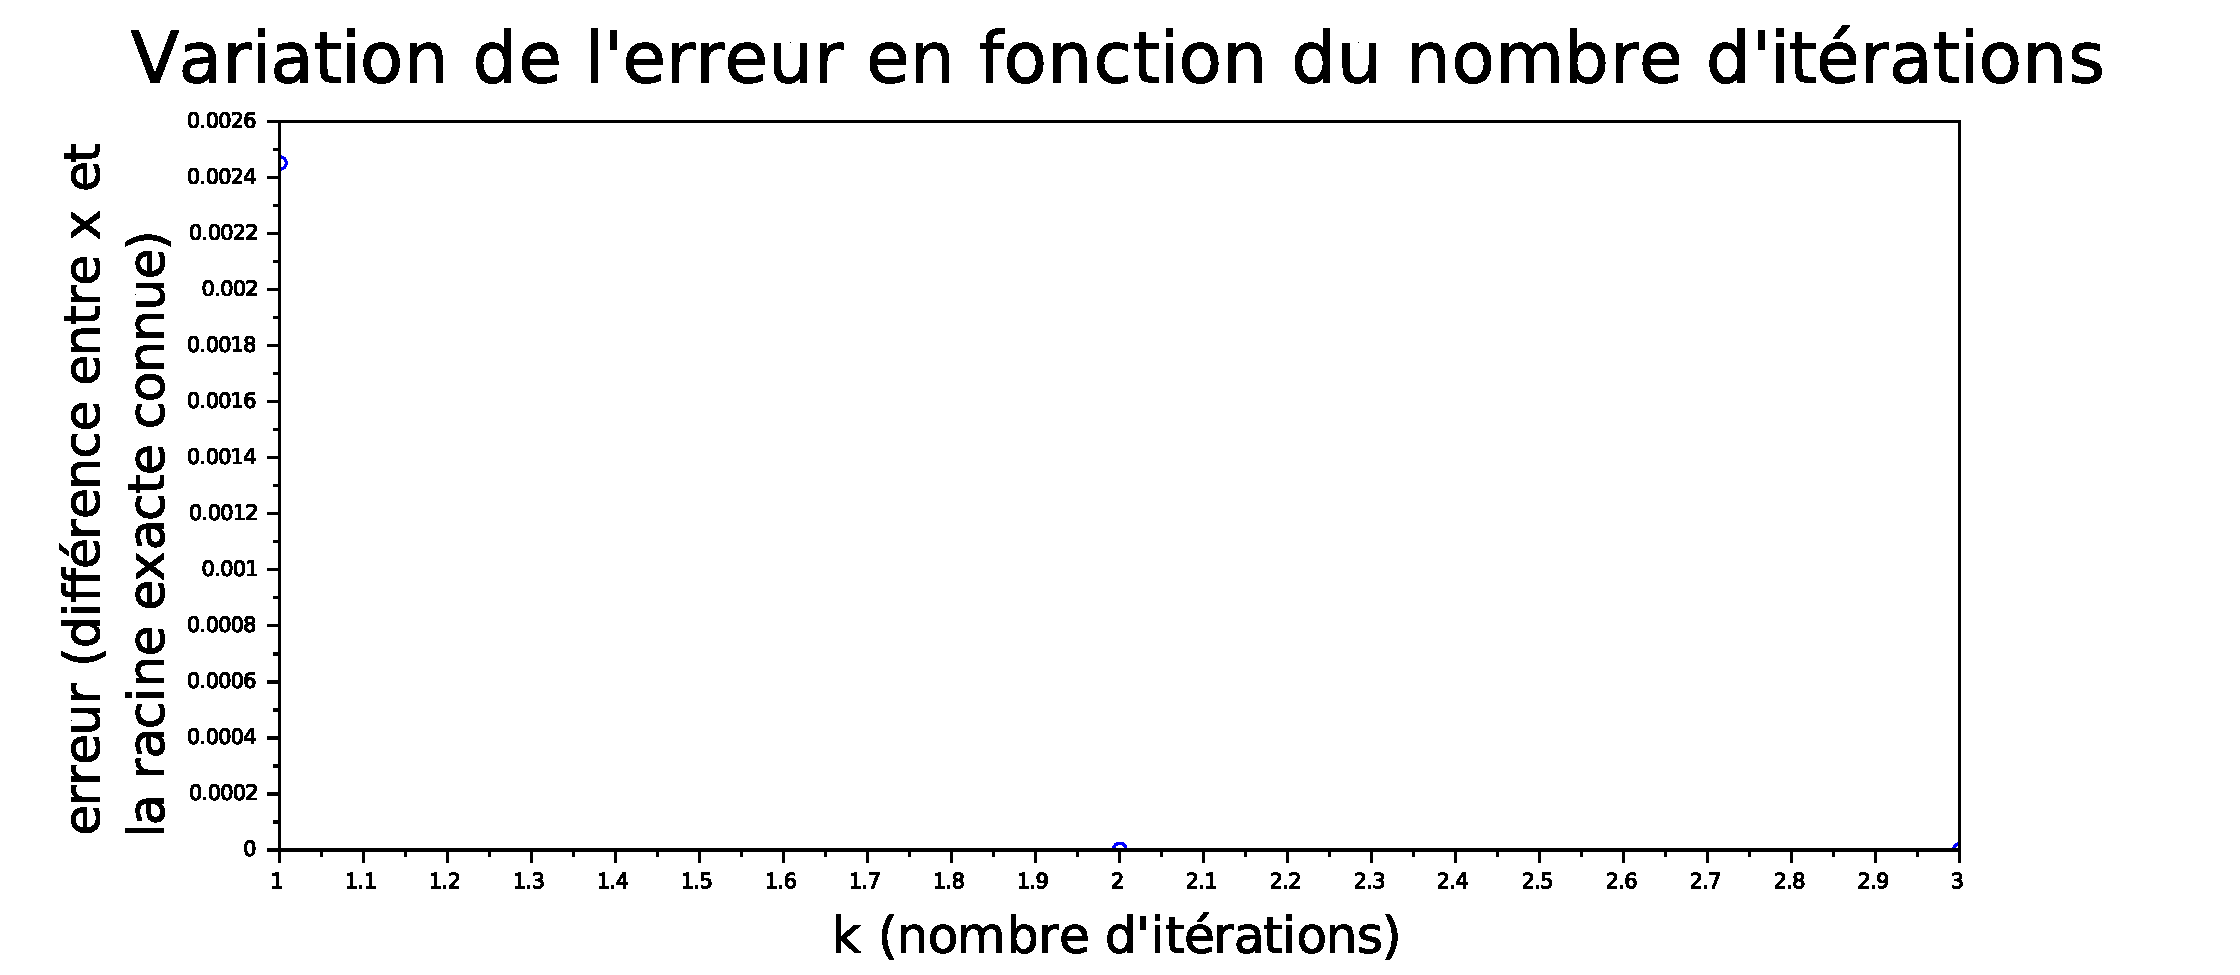
\includegraphics[width=\textwidth]{graphnewton.pdf}
\label{graph_newton}
\end{figure}

Puis on s'intéresse à l'évolution de l'erreur relative (figure \ref{erreur_newton}).
\begin{figure}[H]
\centering
\caption{Diminution relative de l'erreur en fonction de l'itération}
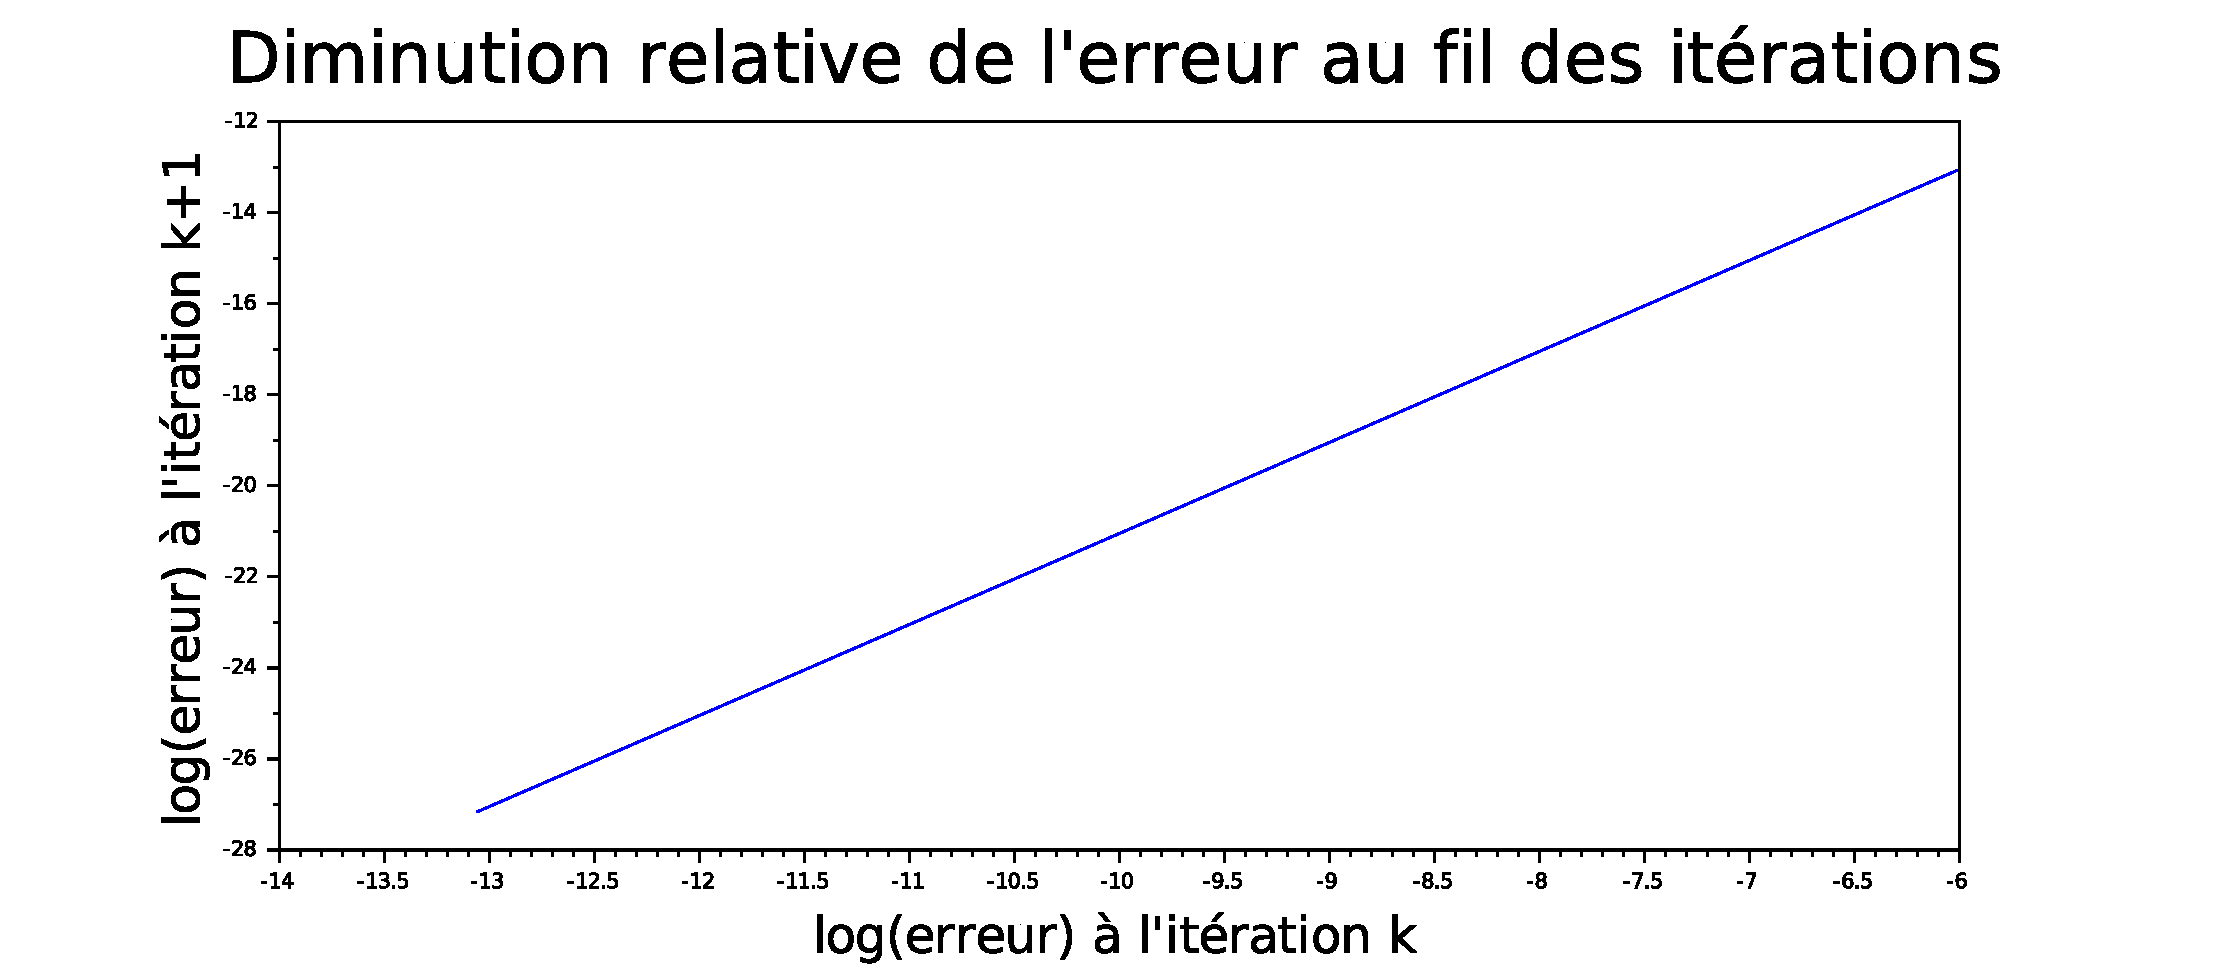
\includegraphics[width=\textwidth]{graphnewton_reg.pdf}
\label{erreur_newton}
\end{figure}

La solution est donc approchée en 3 itérations. Si on linéarise cette courbe (figure \ref{erreur_newton}) grâce à \textit{Scilab}, on obtient un coefficient très proche de 2 (environ 1,9998), il s'agit effectivement d'une convergence quadratique ou d'ordre 2.

\newpage
\section{La méthode de la sécante}
\subsubsection{Théorie}
Comme nous l'avons évoqué précedemment, la méthode de la sécante est directement dérivée de la méthode de Newton.
En effet, dans l'algorithme, on prenait $x_n+1=x_n-\frac{f(x_n}{f-(x_n)}$. Pour la méthode de la sécante, il suffit d'approcher $f'(x_n)$ par le taux d'accroissement, à savoir $\frac{f(x_n)-f(x_{n+1}}{x_n-x_{n+1}}$.\\ \\
L'algorithme devient donc, pour $x_0$ et $x_1$ donnés :
\begin{algorithm}
\begin{algorithmic}
\WHILE{$|f(x_n)|>\varepsilon$}
\STATE $x_{n+1} =  x_{n}-\frac{f(x_n)}{f(x_n)-f(x_{n+1})}(x_n-x_{n+1})$
\ENDWHILE
\end{algorithmic}
\end{algorithm}

\subsubsection{Application}
On étudie une dernière fois $f : \mathbb{R} \longrightarrow \mathbb{R}$ telle que $f(x)=x^2-2$. Comme précédemment, on choisit l'intervalle $[a,b]=[x_0,x_1]=[1,2]$. On implémente donc dans \textit{Scilab} le code \ref{code_secante}.

\begin{table}[H]
\caption{Sécante}
\label{code_secante}
\begin{tabular}{l}
\lstinputlisting[language=scilab]{secante.sce}\\
\end{tabular}
\end{table}

\begin{center}
\begin{figure}[H]
\caption{Erreur en fonction de l'itération}
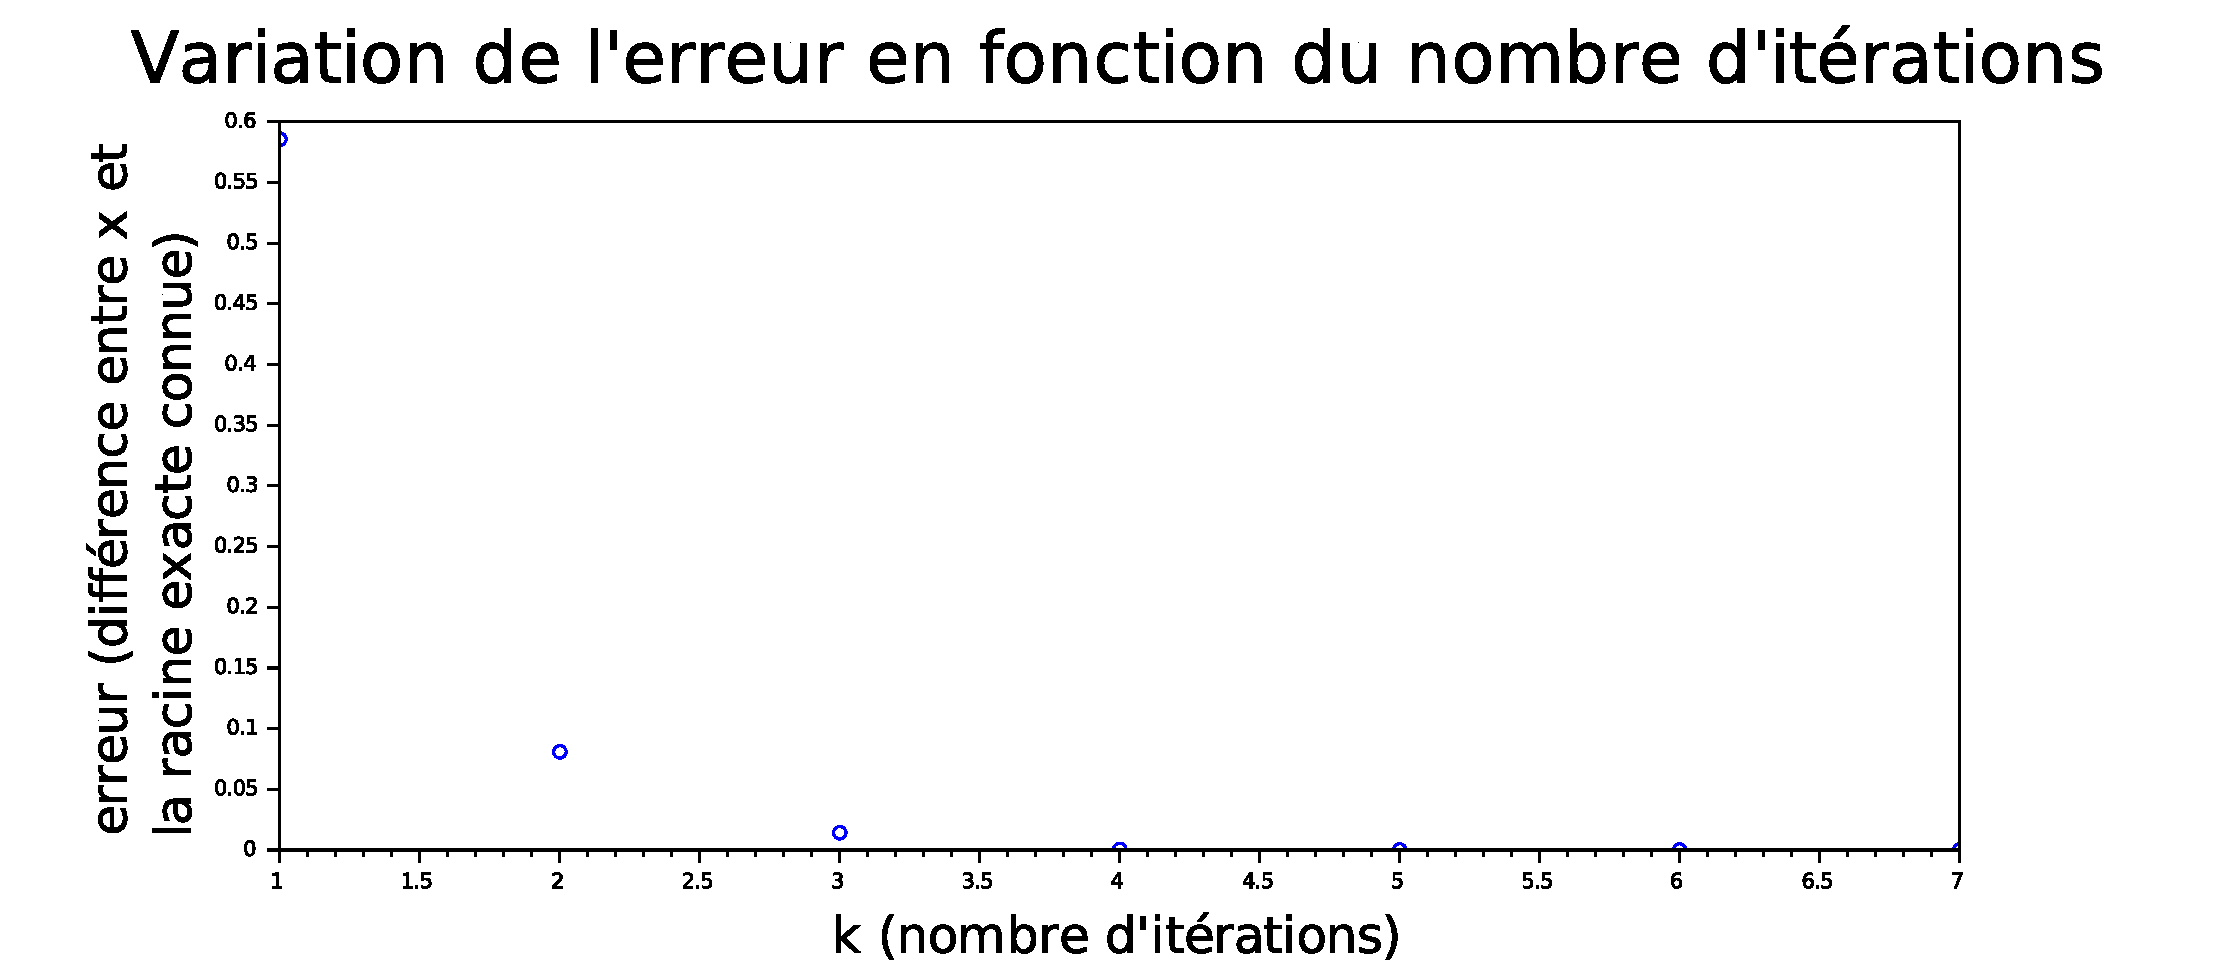
\includegraphics[width=\textwidth]{graphsecante.pdf}
\end{figure}

\begin{figure}[H]
\caption{Diminution relative de l'erreur en fonction de l'itération}
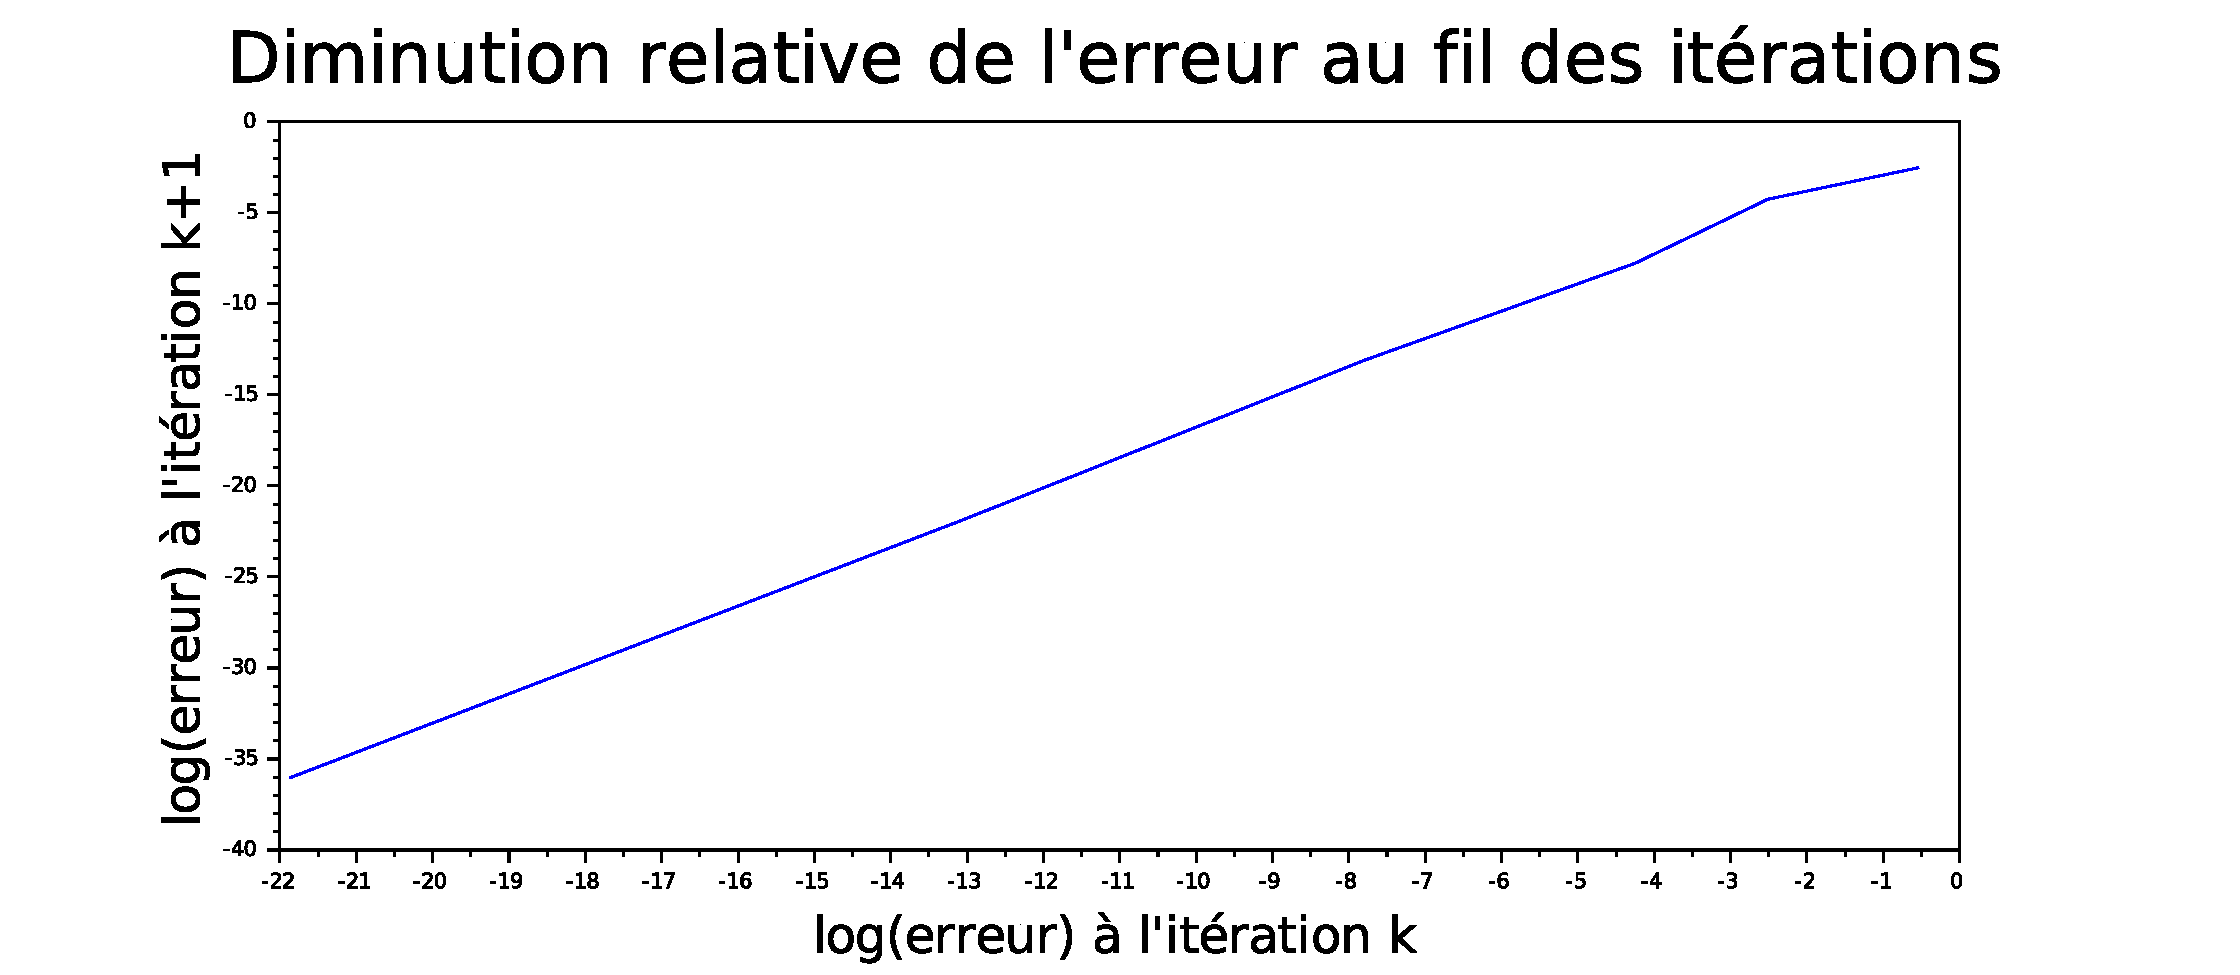
\includegraphics[width=\textwidth]{graphsecante_reg.pdf}
\label{erreur_secante}
\end{figure}
\end{center}

La solution est donc approchée en 7 itérations. Si on linéarise cette courbe (figure \ref{erreur_secante}) grâce à \textit{Scilab}, on obtient un coefficient d'environ 1,6004, il s'agit effectivement d'une convergence d'ordre $\frac{1+\sqrt{5}}{2}$ (le nombre d'or).

\newpage
\section{Pour $n>1$ : La méthode de Newton}
Il existe bien d'autres méthodes afin d'approcher numériquement la solution d'une équations à plusieurs inconnues sous la forme de $f(x) = \left( \begin{array}{c} f_{1}(x) \\ \colon \\ f_{n}(x) \end{array} \right)=0$ avec $f : \mathbb{R} \longrightarrow \mathbb{R}$. La seule méthode dont nous étudierons la partie théorique est la méthode de Newton, appliquée donc dans un cas multidimensionnel.

\subsection{Théorie}
Pour comprendre cette méthode, il apparaît judicieux de revenir sur la notion de différentiabilité. \\
Soit $f : \mathbb{R}^n \longrightarrow \mathbb{R}^n$ avec $f(x) = \left( \begin{array}{c} f_{1}(x) \\ \colon \\ f_{n}(x) \end{array} \right)$ et $x_0\in\mathbb{R}$.\\
On dit que $f$ est différentiable en $x_0$ s'il existe une matrice $A \in \mathcal{M}_{n,n}$ telle que \\
$\forall h\in \mathbb{R}^n$, $f(x_0+h)=f(x_0)+Ah+||h||\varepsilon(h)$ \\ où $\lim\limits_{h \rightarrow \overrightarrow{0}} \varepsilon(h) = \overrightarrow{0}$ et $||h|| \overset{def}{=} \left( \sum \limits_{i=1}^n h_i^2 \right)^\frac{1}{2}$.\\
Les coefficients de $A$ seront alors $a_{i\j}=\frac{\partial f_i}{\partial x_j}(x_0)$.\\
On note $A \overset{def}{=} J_f(x_0)$, $A$ est la matrice Jacobienne de $f$ en $x_0$.\\
\indent De manière analogue au développement de la partie unidimensionnelle, pour $x_0$ donné et $x\in \mathbb{R}$, on a :\\
$f(x)=f(x_0)+J_F(X_0)(x-x_0) + ||x-x_0||\varepsilon(x-x_0)$\\
On effectue l'approximation affine de $f(x)$ : $T_{x_0}(x)=f(x_0)+J_F(x_0)(x-x_0)$\\
On définit $x_1$ par $T_{x_0}(x_1) = \overrightarrow{0}$ (il s'agit d'un système linéaire de n équations à n inconnues)\\
$\Leftrightarrow f(x_0) + J_f(x_0)(x_1-x_0)=\overrightarrow{0} \Leftrightarrow J_f(x_0)(x_1-x_0)=-f(x_0)$\\
d'où $x_1=x_0-\left( J_f(x_0) \right)^{-1}f(x_0)$\\ \\
\indent L'idée de la méthode de Newton est alors la suivante (notons que dans la pratique, on n'inverse pas la matrice, on résout le système d'équation linéaire), pour $x_0$ donné,

\begin{algorithm}
\begin{algorithmic}
\WHILE{$||f(x_n)||>\varepsilon$ \AND $J_{f}(x_{n}) \ est \ inversible$}
\STATE $r\acute{e}soudre \ J_{f}(x_{n})h_{n}=-f(x_{n})$
\STATE $x_{n+1} =  x_{n}+h_{n}$
\ENDWHILE
\end{algorithmic}
\end{algorithm}

\subsection{Fonction \textit{fsolve}}
Avant de commencer l'application de la méthode de Newton, il apparaît judicieux de présenter la macro \textit{fsolve} de \textit{Scilab}. En effet, \textit{Scilab} possède déjà une méthode de résolution des problèmes non linéaires inspirée de la méthode de Newton. \textit{fsolve} a différents prototypes, les arguments qui nous intéressent ici sont :
\begin{itemize}
\item le $x_0$ donné
\item la fonction $f$
\item (facultativement) sa dérivée (\textit{resp.} sa Jacobienne) $df$
\end{itemize}
Si le dernier paramètre, nécessaire à l'application de la méthode de Newton, n'est pas renseigné, \textit{Scilab} ne pouvant la calculer directement, il va l'approcher grâce au développement de Taylor Lagrange.\\
\indent Ainsi, la résolution d'un problème non linéaires avec \textit{Scilab} peut se ramener à la mise en forme du problème sous sa forme standard, $f : \mathbb{R}^n \longrightarrow \mathbb{R}^n$, $f(x)=\overrightarrow{0}$ puis à l'utilisation de la macro \textit{fsolve}.

\subsection{Application 1 : le GPS}

\subsubsection{Énonce et passage en forme standard}
Le sujet de ce problème est le suivant :\\
\indent "Le GPS est un système de positionnement basé sur la connaissance de la distance du récepteur R à trois satellites (situés à des orbites de l’ordre de 	28000km). On suppose que les trois satellites au moment du calcul de distance ont les positions suivantes dans un repère cartésien d’origine le centre de la terre:\\
$S_1 = (-11716.227778, -10118.754628, 21741.083973)$ (unité=km)\\
$S_2 = (-12082.643974, -20428.242179, 11741.374154)$\\
$S_3 = (14373.286650, -10448.439349, 19596.404858)$\\
Sachant que les trois distances respectives au récepteur ont été calculées et valent : $(d_1, d_2, d_3) = (22163.847742, 21492.777482, 21492.469326)$,\\
Déterminer avec \textit{fsolve} la position du récepteur (et vérifier que celui-ci se trouve bien à la surface de la terre...)."\\
\\
\indent Notons $X$ la position du récepteur avec $X= \left( \begin{array}{c} x \\ y \\ z \end{array} \right)$.\\
Le problème nous donne donc le système suivant :
$
\left\lbrace
\begin{array}{l}
||S_1-X||=d_1\\
||S_2-X||=d_2\\
||S_3-X||=d_3\\
\end{array}\right.
$\\
Avec $||X||=\sqrt{x^2+y^2+z^2}$ (il s'agit de la norme euclidienne). La racine carrée pose problème, car la fonction $f : \mathbb{R} \longrightarrow \mathbb{R}$, $f(x)=\sqrt{x}$ n'est pas dérivable sur $\mathbb{R}$. On élève donc chacune des équations du système au carré.
La fonction que l'on cherche donc à annuler dans notre étude est :\\
$f: \mathbb{R}^3 \longrightarrow \mathbb{R}^3$, $f(X)=\left( \begin{array}{c} ||S_1-X||^2-d_1^2 \\ ||S_2-X||^2-d_2^2 \\ ||S_3-X||^2-d_3^2 \end{array} \right)$.\\ \\
\indent Avec \textit{Scilab} comme outils, plusieurs solutions s'offrent donc à nous pour résoudre le problème :
\begin{itemize}
\item utiliser la fonction \textit{fsolve} sans renseigner la Jacobienne
\item calculer la Jacobienne et utiliser la fonction \textit{fsolve} en la renseignant
\item calculer la Jacobienne et appliquer la méthode de Newton (sans utiliser \textit{fsolve})
\end{itemize}
Il peut être intéressant de comparer ces différentes méthodes.

\subsubsection{Méthode 1}
Pour la première méthode, il suffit de renseigner la fonction et de faire appel à \textit{fsolve}. On implémente donc dans \textit{Scilab} le code \ref{GPS1}.

\begin{table}[H]
\caption{GPS (Méthode 1)}
\begin{tabular}{l}
\lstinputlisting[language=scilab]{GPS_1.sce}\\
\end{tabular}
\label{GPS1}
\end{table}

On obtient l'affichage suivant : \begin{verbatim}
-->exec('/home/marlow/latex/GPS_1.sce', -1)
    595.02505  
  - 4856.0251  
    4078.33
\end{verbatim}

\subsubsection{Méthode 2}
Cette méthode ne se différencie pas beaucoup dans la première, la seule différence est que l'on renseigne la Jacobienne en argument de \textit{fsolve}.\\
Calcul de la Jacobienne :\\
Pour simplifier le calcul, on s'intéresse à la première composante de $f(X)$ (à la constante près):\\ $f_1(X) : \mathbb{R}^3 \longrightarrow \mathbb{R}$ avec $f_1(X)=||X-S_1||^2$
\begin{align*}
   f_1(X+h) & = ||(X+h)-S_1||^2 \\
   & = ((X-S_1)+h)^T((X-S_1)+h) \\
   & = (X-S_1)^T(X-S_1) + h^T(X-S_1) + (X-S_1)^Th +h^Th \\
   & = ||X-S_1||^2 + 2(X-S_1)^Th +||h||^2 \\
   & = f_1(X) + J_{f_1}(X) + ||h||\varepsilon(h)
\end{align*}
On peut raisonner de la même façon pour les autres composantes de $f(X)$, on obtient donc :\\
$J_f(X) = \left[ \begin{array}{c} (X-S_1)^T \\ (X-S_2)^T \\ (X-S_3)^T \end{array} \right]$\\
Ainsi, on peut implémenter la Jacobienne dans notre précédent programme \textit{Scilab} et la renseigner dans les arguments de \textit{fsolve}, on obtient le code \ref{GPS2}.

\begin{table}[H]
\caption{GPS (Méthode 2)}
\begin{tabular}{l}
\lstinputlisting[language=scilab]{GPS_2.sce}\\
\end{tabular}
\label{GPS2}
\end{table}

On obtient l'affichage suivant :
\begin{verbatim}
-->exec('/home/marlow/latex/GPS_2.sce', -1)
    595.02505  
  - 4856.0251  
    4078.33   
\end{verbatim}

\subsubsection{Méthode 3}
Enfin, pour tirer parti au maximum de cet exemple, nous allons résoudre le problème sans faire appel à la macro \textit{fsolve} (car \textit{A vaincre sans péril, on triomphe sans gloire}).\\
La Jacobienne a été calculée pour appliquer la deuxième méthode, on a donc : $f(X)=\left( \begin{array}{c} ||S_1-X||^2-d_1^2 \\ ||S_2-X||^2-d_2^2 \\ ||S_3-X||^2-d_3^2 \end{array} \right)$ et
$J_f(X) = \left[ \begin{array}{c} (X-S_1)^T \\ (X-S_2)^T \\ (X-S_3)^T \end{array} \right]$\\
On implémente donc la méthode de Newton dans \textit{Scilab} le code \ref{GPS3}, suivant l'algorithme que nous en avions donné dans la partie théorique.

\begin{table}[H]
\caption{GPS (Méthode 3)}
\begin{tabular}{l}
\lstinputlisting[language=scilab]{GPS_3.sce}\\
\end{tabular}
\label{GPS3}
\end{table}

On obtient l'affichage suivant : \begin{verbatim}
-->exec('/home/marlow/latex/GPS_3.sce', -1)
    595.02505  
  - 4856.0251  
    4078.33    
\end{verbatim}
Cette méthode nous permet de connaître précisément le nombre d'itérations nécessaire pour approcher la solution : $k=10$ après exécution du programme.

\newpage
\subsubsection{Bilan}
Les trois méthodes nous offrent exactement la même solution suivant l'affichage standard de Scilab. On pourrait chercher des différences à quelques décimales prés entre les différentes méthodes, comme on pourrait chercher à connaître le nombre d'itérations (ou d'appels aux fonctions) nécessaires à chaque algorithme avant d'approcher la solution. Toutefois, ce n'est pas vraiment l'objectif qui était fixé, nous nous en tiendrons donc là pour le GPS.\\
Petite remarque : vérifions tout de même que la position que nous avons correspond à une position qui a du sens. En effet, le sujet nous invitait à vérifier que le recepteur se trouve bien à la surface de la Terre : on calcule donc la norme euclidienne de X (notre solution) :
\begin{verbatim}
-->norm(X)
 ans  =
    6369.2864  
\end{verbatim}
Si on suppose un rayon de la Terre égal à 6 371 km (réponse de \textit{Google}), on obtient bien un récepteur GPS à la surface de la Terre.
\\ \\ \\

\subsection{Application 2 : la cinématique inversée}

\subsubsection{Énonce et passage en forme standard}
Le sujet de ce problème est le suivant :\\
\indent "On considère un bras robot articulé dans le plan $(x_1,x_2)$, d’origine $O$, avec un premier segment de longueur $l_1$ et faisant un angle $\theta_1$ avec $(0,x_1)$ et un deuxième segment de longueur $l_2$ faisant un angle $\theta_2$ avec le premier segment. L’extrémité du bras a pour coordonnées :\\
$M(\theta) = (l_1 cos \theta_1 + l_2 cos(\theta_1 + \theta_2 ), l_1 sin \theta_1 + l_2 sin(\theta_1 + \theta_2 ))$.\\
1. Écrire une macro \textit{Scilab} déterminant $\theta$ tel que $M(\theta) = A$ où $A=(x_A,y_A)$ est un point du plan.
2. On prend $l_1 = l_2 = 1$. Écrire un programme \textit{Scilab} utilisant \textit{fsolve} et représentant les positions successives du bras lorsque le point $A(t)$ est défini par une courbe paramétrique, par exemple :\\
$A(t) = \left\lbrace \begin{array}{c} x_1(t)=1+\frac{1}{2}cos(t) \\ x_2(t)=1+\frac{1}{2}sin(t) \end{array} \right.$"\\
\\
\indent Le problème nous donne donc le système suivant :\\
$M(\theta)=A \Leftrightarrow
\left\lbrace
\begin{array}{l}
l_1 cos \theta_1 + l_2 cos(\theta_1 + \theta_2 ) = x_A \\
l_1 sin \theta_1 + l_2 sin(\theta_1 + \theta_2 ) = y_A
\end{array}\right.
$\\
La fonction que l'on cherche donc à annuler dans notre étude est :\\
$f: \mathbb{R}^2 \longrightarrow \mathbb{R}^2$, $f(\theta)=\left( \begin{array}{c} l_1 cos \theta_1 + l_2 cos(\theta_1 + \theta_2 ) - x_A \\ l_1 sin \theta_1 + l_2 sin(\theta_1 + \theta_2 ) - y_A  \end{array} \right)$.\\
\\
Tout comme avec l'application du GPS, plusieurs solutions s'offrent à nous pour résoudre le problème. Toutefois, se contenter d'utiliser la macro \textit{fsolve} ne permet pas d'apprécier l'exécution de la méthode de Newton, itération après itération.

\subsubsection{Calcul de la Jacobienne}
Pour calculer la Jacobienne de la fonction, nous allons utiliser sa définition précédemment énoncée, c'est à dire :\\
$Jf(\theta)=A$ avec $A$ une matrice dont les coefficients sont $a_{i\j}=\frac{\partial f_i}{\partial \theta_j}(\theta)$\\
Par simple calcul de dérivées partielles, on obtient donc :\\
$f(\theta)=\left( \begin{array}{ll}
-l_1 sin \theta_1 - l_2 sin(\theta_1 + \theta_2 ) & -l_2sin(\theta_1+\theta_2) \\
l_1 cos \theta_1 + l_2 cos(\theta_1 + \theta_2 ) & l_2cos(\theta_1+\theta_2)
 \end{array} \right)$

\newpage
\subsubsection{Résolution}
On retranscrit donc à nouveau l'algorithme de la méthode de Newton appliquée à notre exemple dans \textit{Scilab}. On obtient donc le code \ref{code_cinematique}.
\begin{table}[H]
\caption{Cinématique inversée (code principal)}
\begin{tabular}{l}
\lstinputlisting[language=scilab]{cinematique_bis.sce}\\
\end{tabular}
\label{code_cinematique}
\end{table}

\subsubsection{Code fourni pour un rendu graphique}
Le code \textit{dessine\_ bras} appelé pour le rendu graphique est le code \ref{rendu_graphique}.
\begin{table}[H]
\caption{Cinématique inversée (code graphique)}
\begin{tabular}{l}
\lstinputlisting[language=scilab]{dessine_bras.sce}\\
\end{tabular}
\label{rendu_graphique}
\end{table}

\newpage
\subsubsection{Affichage}
On peut ainsi avoir accès après exécution du programme principal à un affichage dynamique de la position du bras à chaque itération. On peut par ailleurs faire varier le nombre d'itérations pour construire plus de bras (figure \ref{affichage_cinematique} : affichages pour différentes valeurs de $n$).
\begin{figure}[H]
\caption{Différents affichages de la cinématique inversée en fonction de $n$}
   \begin{minipage}[c]{.48\linewidth}
   \centering
      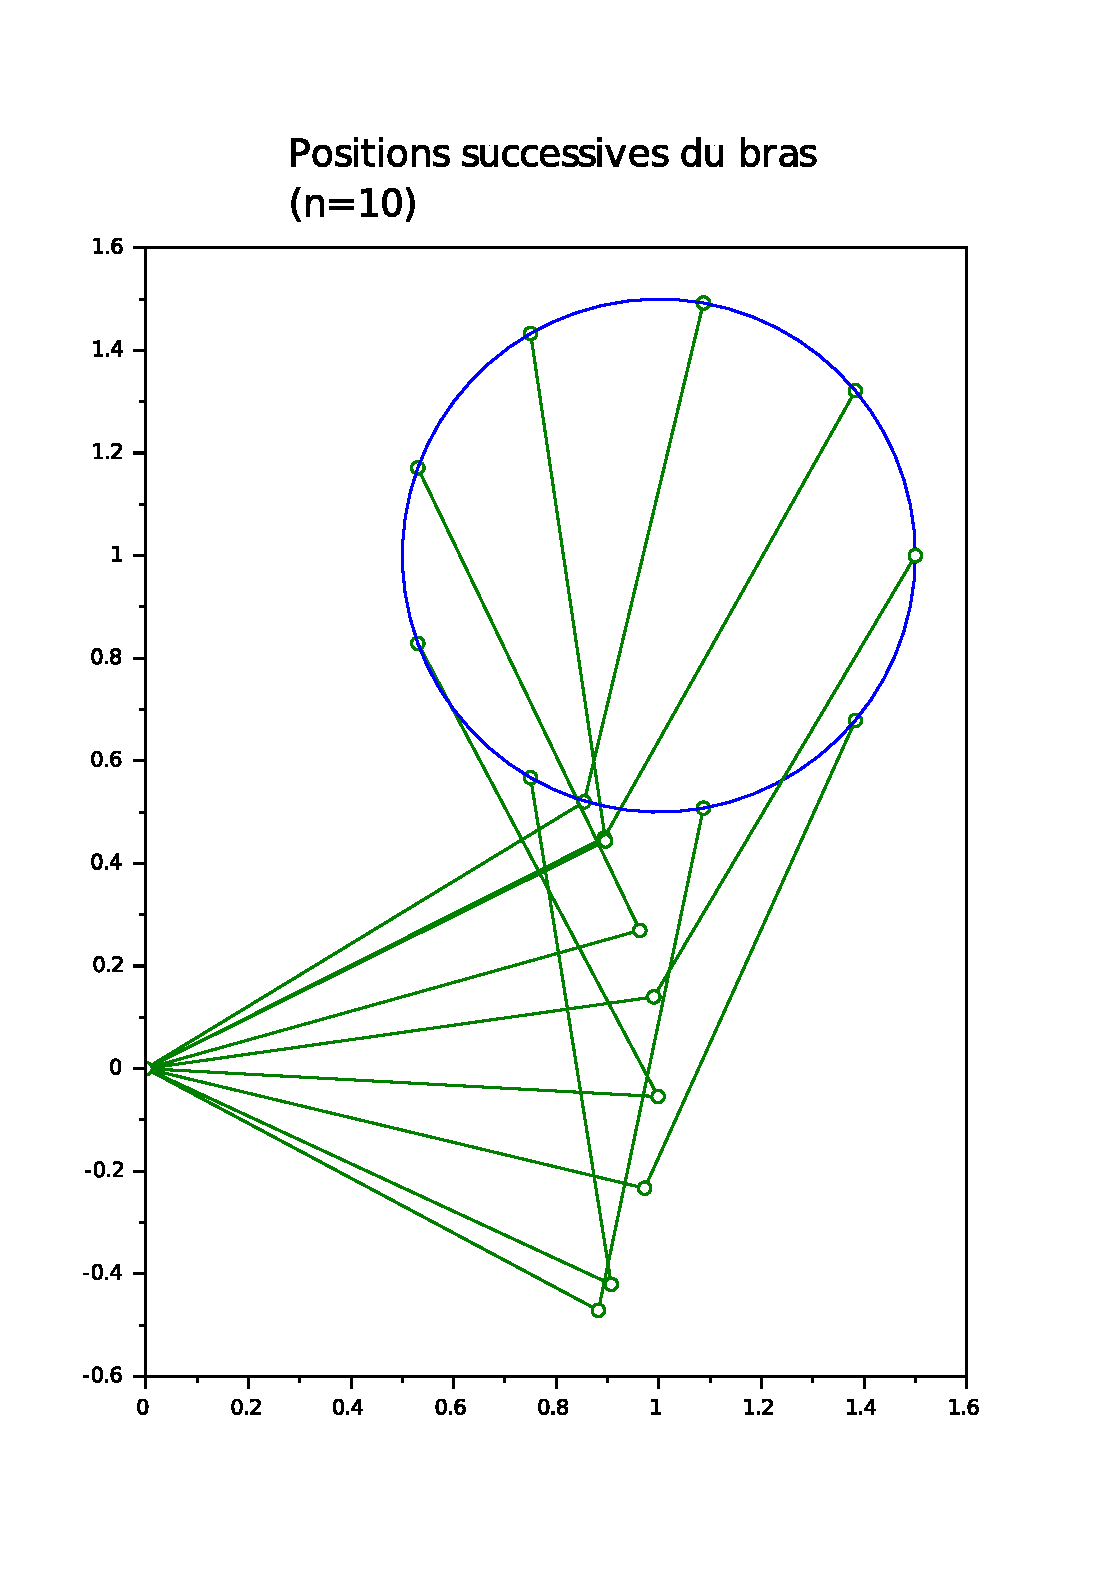
\includegraphics[width=\textwidth]{graphcinematique.pdf}
   \end{minipage} \hfill
   \begin{minipage}[c]{.48\linewidth}
   \centering
      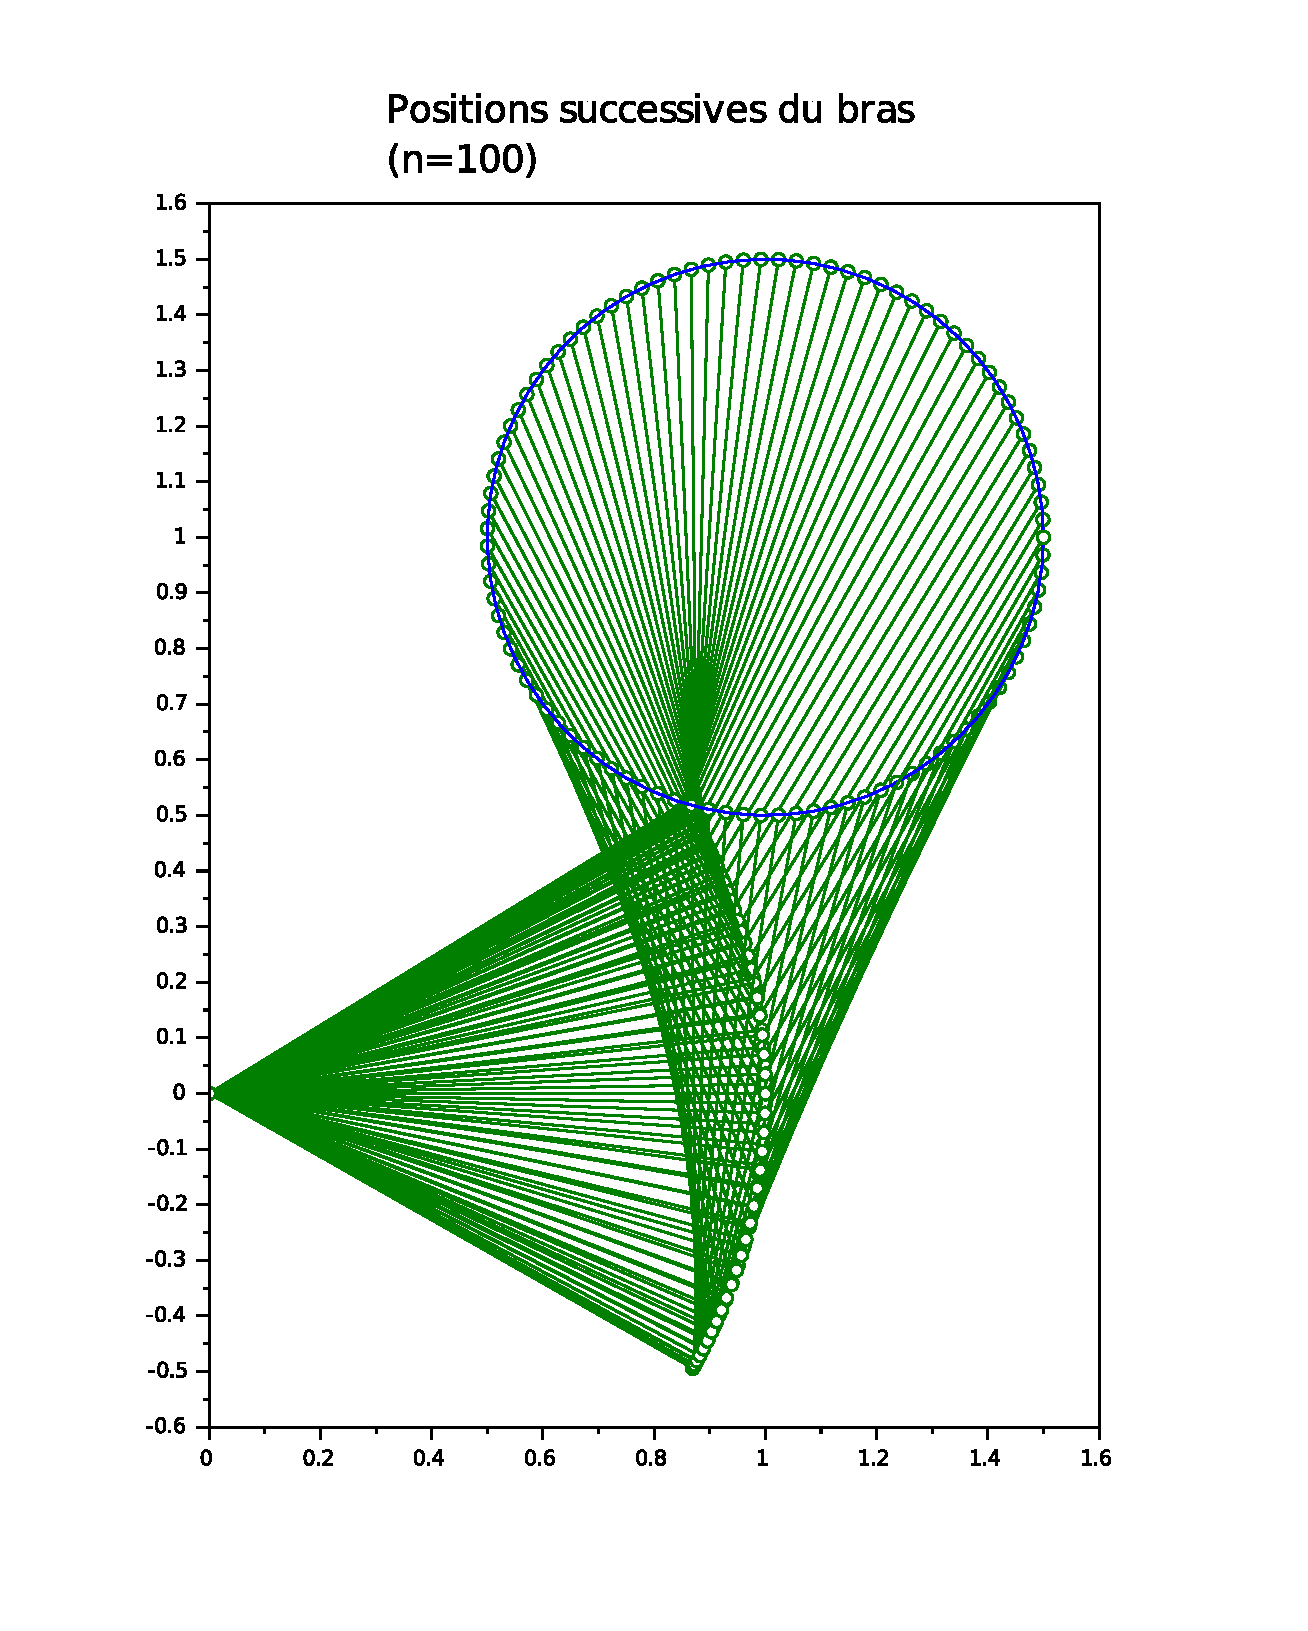
\includegraphics[width=\textwidth]{graphcinematique_2.pdf}
   \end{minipage}
\label{affichage_cinematique}
\end{figure}

\chapter{Fractales}
\section{Introduction}
L'existence des fractales part d'une interrogation assez surprenante : comment construire des figures parfaitement irrégulières, peu importe l'échelle choisie pour les observer (c'est à dire des courbes de fonctions continues mais non dérivables) ? Comment simuler grâce à des outils mathématiques des motifs présent dans la nature comme l'écume des vagues, les nuages,... ? Comment représenter \textit{l'infini} sur une surface finie ? La solution à ces interrogations est d'aller au delà de la géométrie classique, c'est à dire euclidienne.

\begin{center}
\begin{figure}[H]
\caption{Exemple de fractales : fractale de Mandelbrot}
\includegraphics[width=\textwidth]{fractales_intro.jpg}
\end{figure}
\end{center}

\section{Dimension de Hausdorff}
Avant d'étudier des fractales particuliers, il apparaît pertinent de commencer par définir \textit{la dimension de Hausdorff}, c'est à dire la notion de dimension que l'on peut appliquer à un fractal. La dimension de Van Hausdorff d'une fractale $K$ est définie ainsi :\\
\begin{itemize}
\item on note $N(\varepsilon)$ le nombre de carrés de longueur (ou de disques de rayon) $\varepsilon$ recouvrant $K$
\item on a alors $d=\lim\limits_{\varepsilon \rightarrow 0} \frac{ln(N(\varepsilon))}{ln(\frac{1}{\varepsilon})}$, $d \notin \mathbb{N}$
\end{itemize}
Avec cette définition, nous calculerons donc la \textit{dimension de Hausdorff} de chacune des fractales que nous étudierons.

\section{Ensemble de Cantor}
\subsection{Théorie}
\subsubsection{Présentation}
\begin{minipage}[c]{.70\linewidth}
	\indent L'étude de tels objets n'a pas attendu l'apparition du terme "fractale" par Benoît Mandelbrot en 1974. Certains mathématiciens se sont intéressés à 	ces objets avant même de pouvoir les nommer. On considère souvent comme la première figure fractale l'objet construit par le mathématicien allemand Benoît Cantor : \textit{l'ensemble de Cantor}.
	\begin{figure}[H]
	\caption{Ensemble de Cantor}
	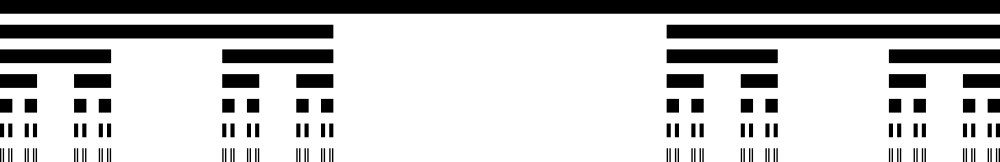
\includegraphics[width=\textwidth]{cantor.png}
	\end{figure}
\end{minipage} \hfill
\begin{minipage}[c]{.05\linewidth}
\end{minipage} \hfill
\begin{minipage}[c]{.21\linewidth}
	\begin{figure}[H]
	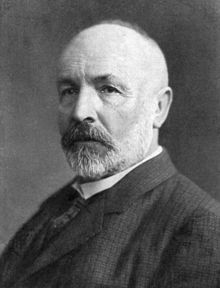
\includegraphics[height=4cm]{mr_cantor.jpg}
	\caption{Cantor 1845-1918}
	\end{figure}
\end{minipage}

\subsubsection{Définition algorithmique}
\begin{algorithm}
\begin{algorithmic}
\REQUIRE{Un segment [0,1]}
\STATE \textbf{Opération de base :} Partager le segment en trois parties égales et ne pas retenir le segment central
\STATE \textbf{Itération :} Itérer l'opération sur chacun des segments retenus
\end{algorithmic}
\end{algorithm}

\subsubsection{Remarques}
On appelle $\mathsf{C^{(k)}}$ l'ensemble obtenu à l'étape $k$, on note : $\mathsf{C^{(\infty)}} = \bigcap^{\infty}_{\mathsf{k}=0}\mathsf{C^{(k)}}$\\
On a par ailleurs les propriétés suivantes :
\begin{align*}
   i) \ & |\mathsf{C^{(\infty)}}|=0 \\
   ii) \ & \mathsf{C^{(\infty)}}\ est\ d\acute{e}nombrable
\end{align*}
On peut démontrer ces propriétés :\\
\textbf{démo \textit{i)}}\\
$|\mathsf{C^{(0)}}|=1$, $|\mathsf{C^{(1)}}|=\frac{2}{3}$, $|\mathsf{C^{(2)}}|=\frac{4}{9}=\left( \frac{2}{3} \right)^2$\\
par récurrence, on obtient $|\mathsf{C^{(k)}}|=\left( \frac{2}{3} \right)^k \Rightarrow \lim\limits_{k \rightarrow \infty} |\mathsf{C^{(k)}}|= 0 \Rightarrow |\mathsf{C^{(\infty)}}|=0$\\

\newpage
\noindent \textbf{démo \textit{ii)}}\\
$\mathsf{C^{(\infty)}}\ est\ en\ bijection\ avec\ [0,1] \Rightarrow \mathsf{C^{(\infty)}}\ est\ d\acute{e}nombrable $\\
Or on a le \textbf{théorème} :\\
$\forall x\in \mathsf{C^{(\infty)}}, x=(0,x_1x_2\cdots x_k\cdots)_3 $ avec $(x)_3$ désigne la base 3 de $x$ et $x_i = 0\ ou\ 2$\\
exemple :
\begin{align*}
   \frac{1}{3} & =(0,1)_3 \ = (0,0222\cdots 2\cdots)_3 = \frac{0}{3} + \frac{2}{3^2} + \frac{2}{3^3} + \cdots + \frac{2}{3^k} + \cdots\\
               & = \frac{2}{3^2} \left( 1 + \frac{1}{3} + \cdots + \frac{1}{3^k} + \cdots \right) = \frac{2}{9} \times \frac{1}{1-\frac{1}{3}} = \frac{2}{9}\times\frac{3}{2}=\frac{1}{3}
\end{align*}
Soit donc la \textbf{bijection} $x \longrightarrow \frac{x}{2}=0,\frac{x_1}{2}\frac{x_2}{2}\cdots\frac{x_k}{2}\cdots$\\
donc $\forall x\in \mathsf{C^{(\infty)}}$ on associe en base 2 le nombre $(0,x_1x_2\cdots x_k\cdots)_2$

\subsubsection{Dimension de l'ensemble de Cantor}
Pour calculer la dimension de l'ensemble de Cantor au sens de la \textit{dimension de Hausdorff}, on compte le nombre de carrés nécessaires à chaque étape pour recouvrir la figure :
\begin{itemize}
\item à l'initialisation, $1$ seul carré de côté $1$
\item à l'itération 1, $2$ carrés de côté $\frac{1}{3}$ sont nécessaires pour recouvrir les segments
\item à l'itération 2, $4=2^2$ carrés de côté $\frac{1}{9} = \frac{1}{3^2}$ sont nécessaires pour recouvrir les segments
\item à l'itération k, $2^k$ carrés de côté $\frac{1}{3^k}$ sont nécessaires pour recouvrir les segments
\end{itemize}
On a donc $d=\lim\limits_{k \rightarrow \infty} \frac{ln(2^k)}{ln(3^k)}=\frac{ln(2)}{ln(3)}$ la dimension de l'ensemble de Cantor.
\\ \\

\subsection{Application dans \textit{Scilab} (méthode récursive)}
La méthode récursive s'inspire directement de l'algorithme de définition de l'ensemble de Cantor. On implémente donc dans \textit{Scilab} le code \ref{code_cantor}.
\begin{table}[H]
\caption{Ensemble de Cantor (méthode récursive)}
\begin{tabular}{l}
\lstinputlisting[language=scilab]{cantor_recursif.sce}\\
\end{tabular}
\label{code_cantor}
\end{table}
L'exécution du code nous donne ainsi la figure \ref{cantor_recursif}.
\begin{center}
\begin{figure}[H]
\centering
\caption{Figure pour n=7}
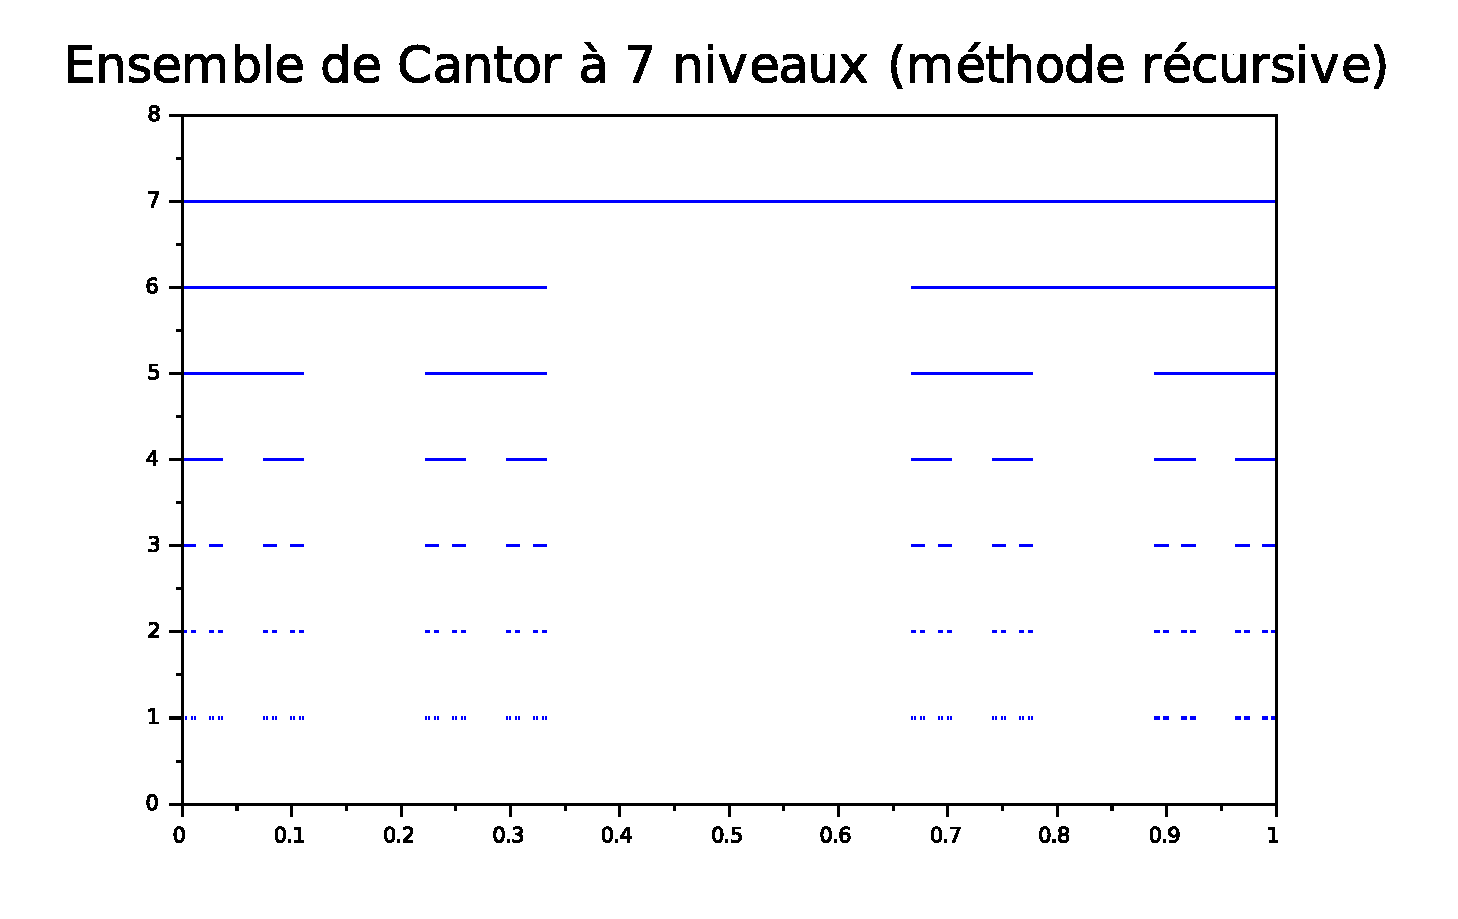
\includegraphics[width=0.8\textwidth]{cantor_recursif.pdf}
\label{cantor_recursif}
\end{figure}
\end{center}

\subsection{Application dans \textit{Scilab} (méthode itérative)}
Même si la méthode récursive appliquée précedemment pour dessiner l'ensemble de Cantor s'est révélée efficace pour $n=7$ niveaux, elle l'est beaucoup moins pour des valeurs de $n$ supérieures. En effet, la complexité de l'algorithme est de l'ordre de $O(2^n)$ (on réalise 2 appels récursifs pour chaque niveau), on dit qu'elle est exponentielle, un tel algorithme est donc de plus en plus \textit{gourmand} en temps et en mémoire à mesure que $n$ augmente. En outre, la complexité des algorithmes récursifs devient rapidement délirante pour tracer des fractales en 2D, encore d'avantage en 3D. C'est pourquoi il est pertinent de s'intéresser dés à présent à d'autres méthodes de dessin des fractales : les méthodes itératives. Nous allons donc étudier l'une d'entre elles : celles des IFS (\textit{Iterated Functions Systems}), en français \textit{les systèmes de fonctions itérées}.\\
\\
\indent La théorie des IFS, basée sur l'invariance par changement d'échelle, permet la représentation fonctionnelle d'un fractale. Cette théorie fait appel à la notion de \textit{fonctions contractantes} sur un espace métrique $M$, (c'est à dire muni d'une notion de distance $d$ entre deux éléments). Graphiquement, une fonction contractante "rapproche les images". Une fonction $f$ est dite \textit{contractante} ou \textit{k-contractante} sur $M(E,d)$ ssi :
\begin{equation}
\exists k, 0\leq k\leq 1, \forall (x,y) \in E^2, d(f(x),f(y))\leq kd(x,y)
\end{equation}
\indent Un IFS est un ensemble de fonctions $f_1,f_2,\cdots f_n$ toutes contractantes sur un ensemble de compacts de $M$ munis de la \textit{distance de Hausdorff}. On définit alors la fonction $f$, avec $A$ un compact, par :
\begin{equation}
f(A)=f_1(A)\cup f_2(A)\cup \cdots \cup f_n(A)
\end{equation}
On peut montrer que $f$ est aussi contractante de rapport de contraction $k=max(k_i)$.

\indent Le \textit{théorème du collage}, démontré par Barnsley en 1985, énonce que tout IFS converge vers un \textit{attracteur} $A$, c'est à dire un ensemble vers lequel le système évolue irrémédiablement, tel que $f(A)=A$ pour tout donnée initiale choisie, $A$ est donc un point fixe de $f$. Autrement dit, un IFS converge vers un compact attracteur $A$ qui se révèle être une fractale.
\\ \\
\indent Pour une fractale particulière, on déduit les fonctions $f_1,f_2,\cdots f_n$ à partir de la définition algorithmique de la fractale. On travaille donc sur un ensemble fini de points, et pour chaque point, on choisit (aléatoirement) d'y appliquer une des fonctions $f_1,f_2,\cdots f_n$. \\

Pour l'ensemble de Cantor, on a :\\
\begin{equation}
\begin{array}{l}
f(C)=f_0(C)\cup f_1(C) \ avec \
\left\lbrace
\begin{array}{l}
f_0,\ f_1 : [0,1] \longrightarrow [0,1] \\
f_0 : x \longrightarrow \frac{x}{3}\\
f_1 : x \longrightarrow \frac{x}{3}+\frac{2}{3}\\
\end{array}\right.
d'o\grave{u} \
\left\lbrace
\begin{array}{l}
C_0 : [0,1]\\
C_{n+1} : f(C_n)\\
\end{array}\right.
\end{array}
\end{equation}
Finalement $C_n$ converge au sens de la distance de Hausdorff vers $C^\infty$, l'ensemble de Cantor. Pour la sélection de la fonction à appliquer à une point particulier, on applique une méthode équiprobable afin d'obtenir un ensemble uniforme.\\ \\
\indent On implémente donc dans \textit{Scilab} le code suivant :
\begin{table}[H]
\caption{Ensemble de Cantor (méthode itérative)}
\begin{tabular}{l}
\lstinputlisting[language=scilab]{cantor_iteratif.sce}\\
\end{tabular}
\end{table}
L'exécution du code nous donne ainsi la figure \ref{cantor_iteratif}.:
\begin{center}
\begin{figure}[H]
\caption{Ensemble de Cantor itératif pour 1000 points}
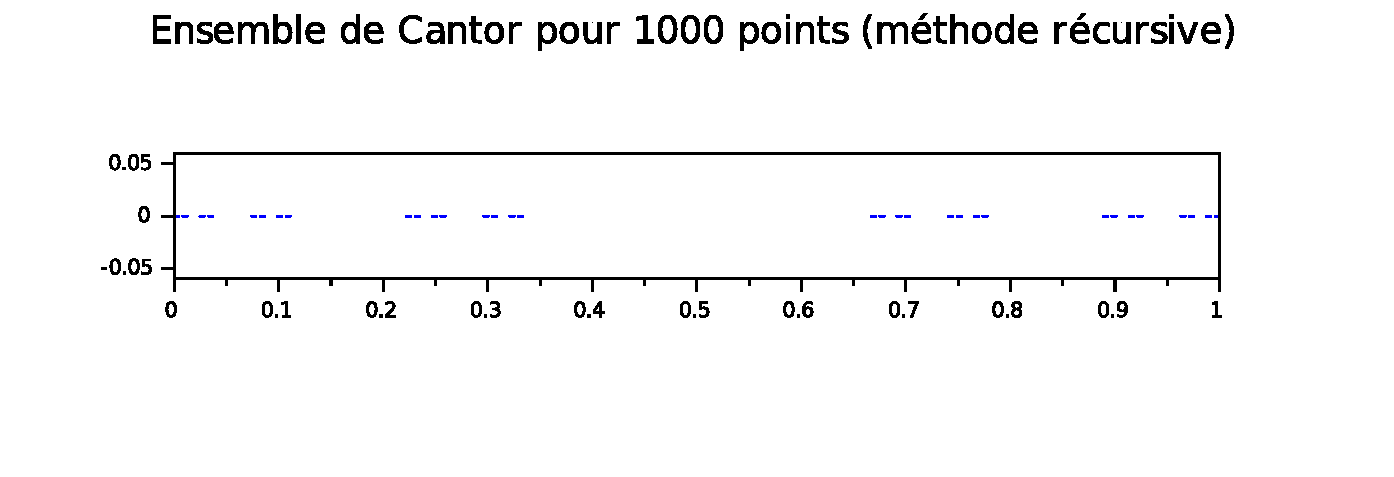
\includegraphics[width=\textwidth]{cantor_iteratif.pdf}
\label{cantor_iteratif}
\end{figure}
\end{center}

\section{Triangle de Sierpinski}
\subsection{Théorie}
\subsubsection{Présentation}
\begin{minipage}[c]{.70\linewidth}
	\indent Notre analyse continue avec l'étude d'une seconde fractale construite par Waclaw Sierpinski, mathématicien polonais, fractale nommée \textit{le triangle de Sierpinski}.
	\begin{figure}[H]
	\centering
	\caption{Triangle de Sierpinski}
	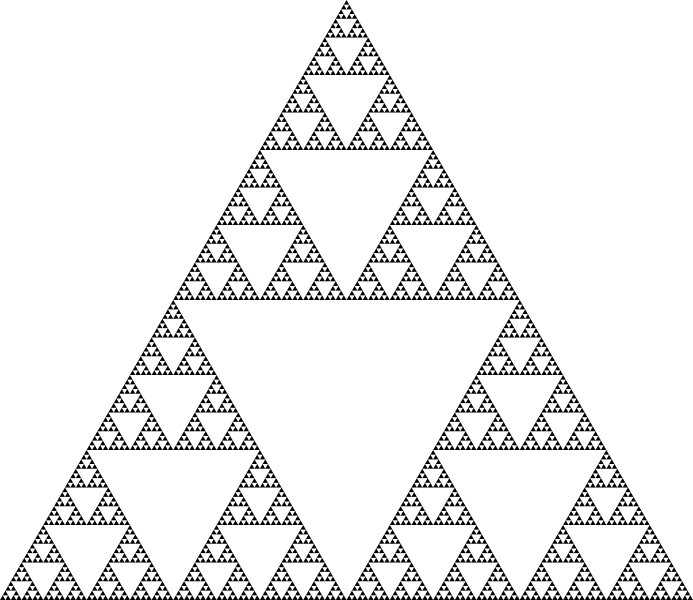
\includegraphics[height=5cm]{sierpinski.png}
	\end{figure}
\end{minipage} \hfill
\begin{minipage}[c]{.05\linewidth}
\end{minipage} \hfill
\begin{minipage}[c]{.21\linewidth}
	\begin{figure}[H]
	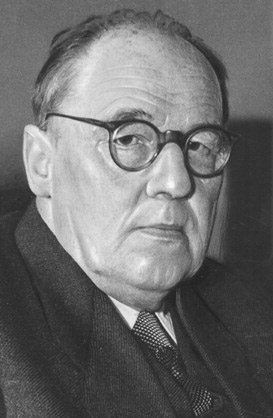
\includegraphics[height=4cm]{mr_sierpinski.jpg}
	\caption{Sierpinski 1882-1924}
	\end{figure}
\end{minipage}

\subsubsection{Définition algorithmique}
\begin{algorithm}
\begin{algorithmic}
\REQUIRE{Un triangle équilatéral de côté 1}
\STATE \textbf{Opération de base :} Partager le triangle en 4 triangles équilatéraux égaux et ne pas retenir le triangle central
\STATE \textbf{Itération :} Itérer l'opération sur chacun des triangles retenus
\end{algorithmic}
\end{algorithm}

\subsubsection{Dimension du Triangle de Sierpinski}
On appelle $T^k$ la figure obtenue à l'itération $k$. On applique donc la définition de la dimension de Hausdorff au triangle de Sierpinski :\\ \\
\begin{tabular}{ccccc}
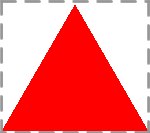
\includegraphics[height=2.4cm]{sierpinski0.png} & $\rightarrow$ & 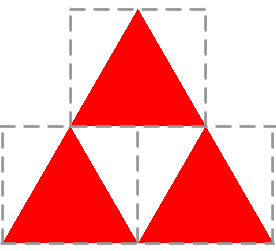
\includegraphics[height=2.5cm]{sierpinski1.png} & $\rightarrow$ & 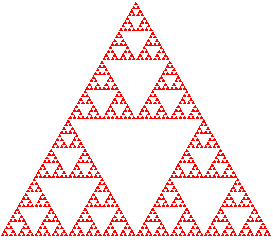
\includegraphics[height=2.5cm]{sierpinskik.png}\\
$T_0$ & & $T_1$ & ... & $T_k$\\
1 seul carré & & 3 carrés & ... & $3^k$ carrés\\
de côté 1 & & de côté $\frac{1}{2}$ & ... & de côté $\varepsilon_k = \frac{1}{2^k}$\\
\end{tabular} \\ \\ \\
Donc $d=\lim\limits_{k \rightarrow \infty} \frac{ln(3^k)}{ln(2^k)}=\frac{ln(3)}{ln(2)}$ est la dimension de Hausdorff du fractal.

\newpage
\subsection{Application dans \textit{Scilab} (méthode récursive)}
Le programme récursif s'inspire tout autant de la définition même de la fractale que celui pour l'ensemble de Cantor. On implémente donc dans \textit{Scilab} le code \ref{code_sierp}.
\begin{table}[H]
\caption{Triangle de Sierpinski (méthode récursive)}
\begin{tabular}{l}
\lstinputlisting[language=scilab]{sierpinski_recursif.sce}\\
\end{tabular}
\label{code_sierp}
\end{table}
L'exécution du code nous donne ainsi la figure \ref{sierpinski_recursif}.
\begin{figure}[H]
\centering
\caption{Triangle de Sierpinski (récursif) pour n=5}
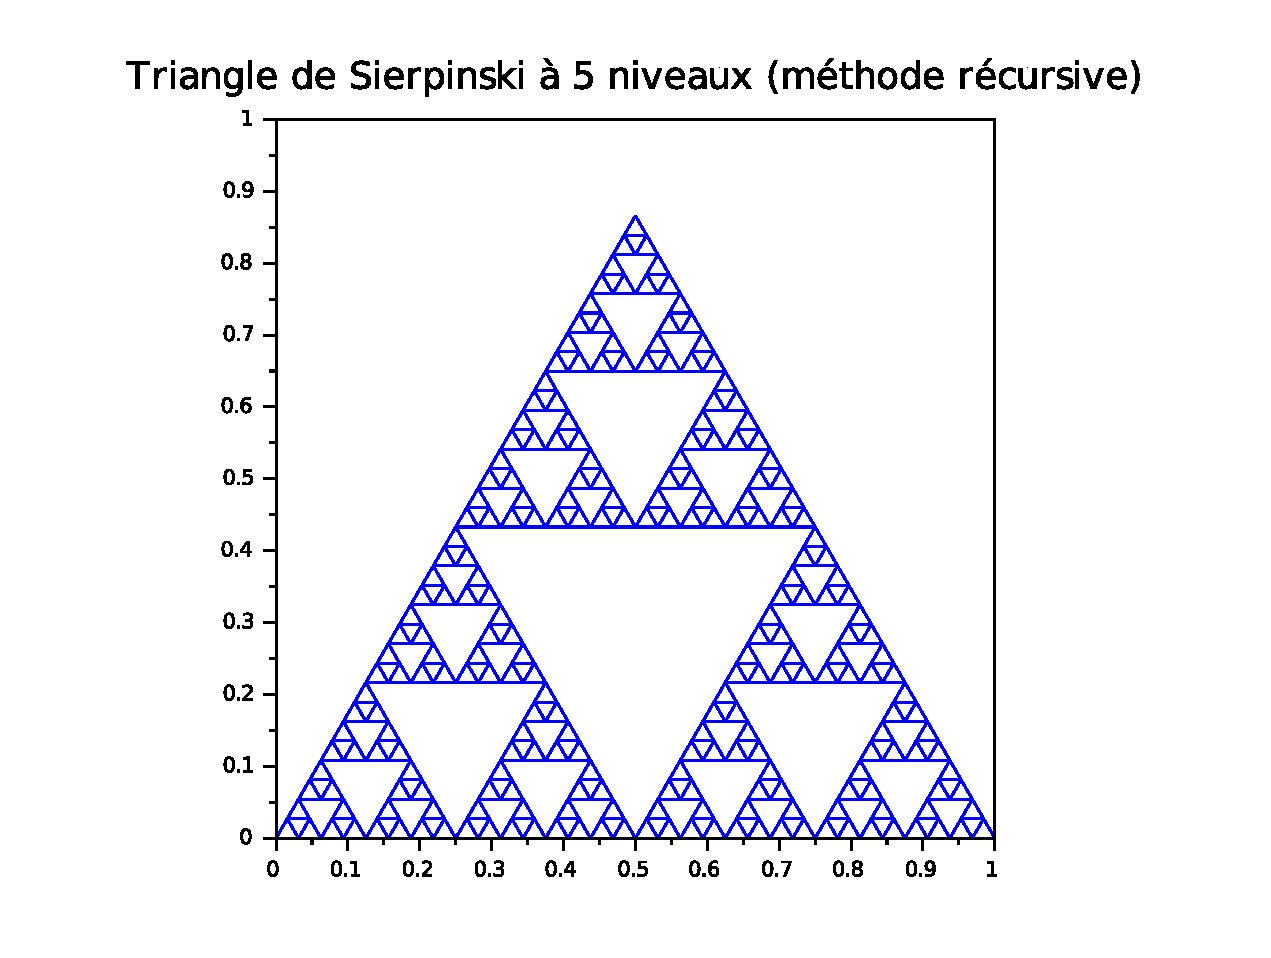
\includegraphics[width=0.75\textwidth]{sierpinski_recursif.pdf}
\label{sierpinski_recursif}
\end{figure}

\newpage
\subsection{Application dans \textit{Scilab} (méthode itérative)}
La complexité de l'algorithme récursif est ici en $O(3^n)$ (on réalise 3 appels récursifs pour chaque niveau). Comme pour l'ensemble de Cantor, cette complexité est surmontable pour des valeurs de niveaux relativement faibles ($n\leq 7$), mais pour des valeurs de $n$ importantes, cette méthode n'est plus applicable. On implémente donc également une méthode itérative à l'aide d'un IFS. On a donc :
\begin{equation}
\left\lbrace
\begin{array}{l}
f_0 \left[ \begin{array}{ll} x \\ y \end{array} \right] =
\left[ \begin{array}{ll} \frac{1}{2} & 0 \\ 0 & \frac{1}{2} \end{array} \right]
\left[ \begin{array}{ll} x \\ y \end{array} \right]\\ \\

f_1 \left[ \begin{array}{ll} x \\ y \end{array} \right] =
\left[ \begin{array}{ll} \frac{1}{2} & 0 \\ 0 & \frac{1}{2} \end{array} \right]
\left[ \begin{array}{ll} x \\ y \end{array} \right]
+ \left[ \begin{array}{ll} \frac{1}{2} \\ 0 \end{array} \right]\\ \\

f_2 \left[ \begin{array}{ll} x \\ y \end{array} \right] =
\left[ \begin{array}{ll} \frac{1}{2} & 0 \\ 0 & \frac{1}{2} \end{array} \right]
\left[ \begin{array}{ll} x \\ y \end{array} \right]
+ \left[ \begin{array}{ll} \frac{1}{4} \\ \frac{\sqrt{3}}{4} \end{array} \right]\\
\end{array}\right.
\end{equation}
$d'o\grave{u} \
\left\lbrace
\begin{array}{l}
T_0 \ donn\acute{e} \\
T_{n+1} : f(T_n) \ avec \ f(T)=f_0(T)\cup f_1(T)\cup f_2(T)\\
\end{array}\right.$\\ \\
Finalement $T_n$ converge au sens de la distance de Hausdorff vers $T^\infty$, le triangle de Sierpinski. A nouveau, la dispersion des points doit être uniforme, on utilise donc des conditions d'équiprobabilité. \\ \\

\indent On implémente donc dans \textit{Scilab} le code \ref{code_sierpinski_it}.
\begin{table}[H]
\caption{Triangle de Sierpinski (méthode itérative)}
\begin{tabular}{l}
\lstinputlisting[language=scilab]{sierpinski_iteratif.sce}\\
\end{tabular}
\label{code_sierpinski_it}
\end{table}
\newpage
L'exécution du code nous donne ainsi la figure \ref{sierpinski_iteratif}.
\begin{figure}[H]
\centering
\caption{Triangle de Sierpinski itératif pour 1000 points}
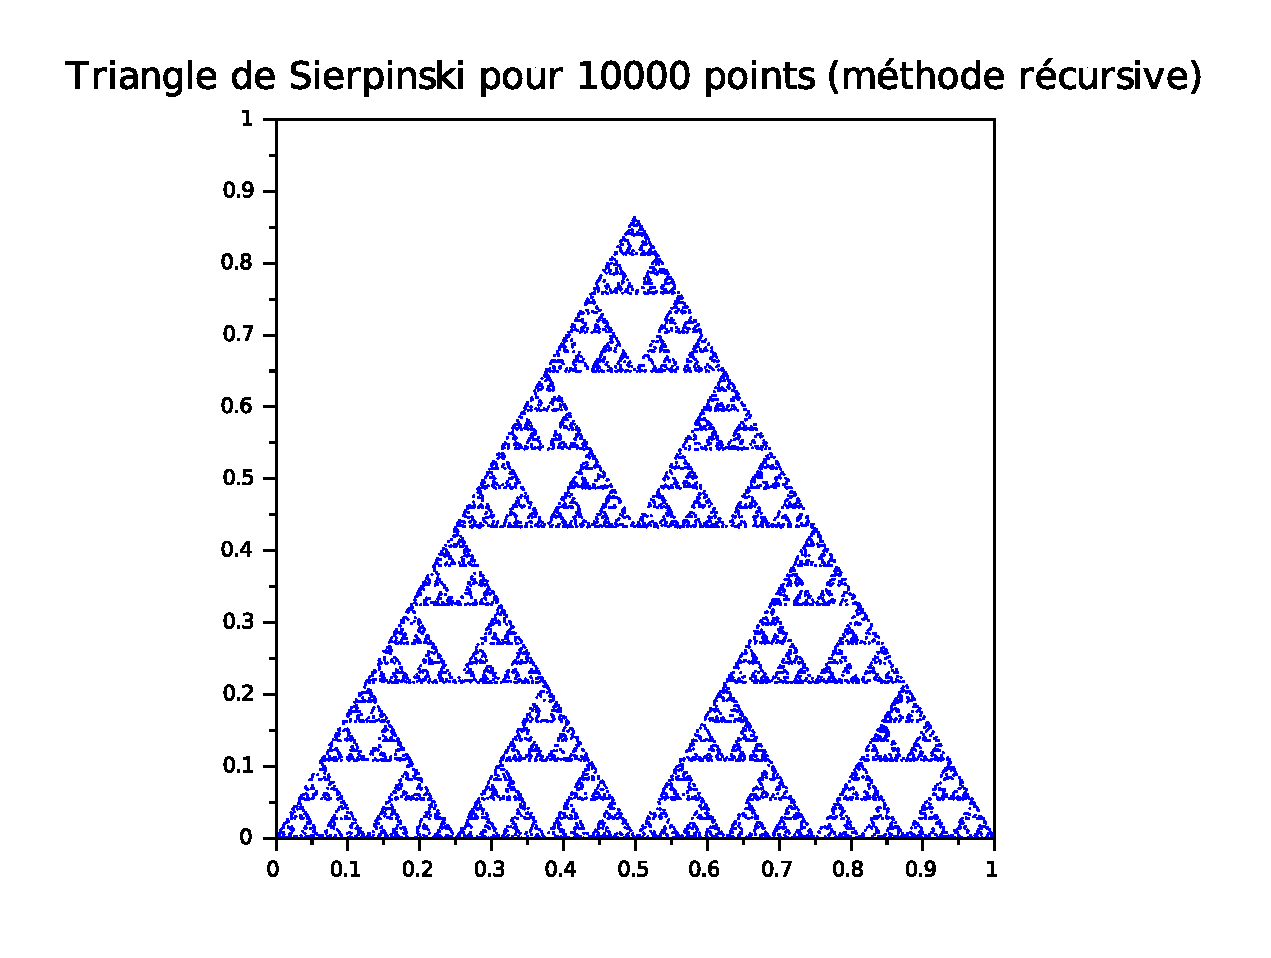
\includegraphics[width=0.75\textwidth]{sierpinski_iteratif.pdf}
\label{sierpinski_iteratif}
\end{figure}

\subsection{Variante : le tapis de Sierpinski}
On a pu travailler sur une variante du triangle de Sierpinski : \textit{Le tapis de Sierpinski}.
\begin{figure}[H]
\centering
\caption{Tapis de Sierpinski}
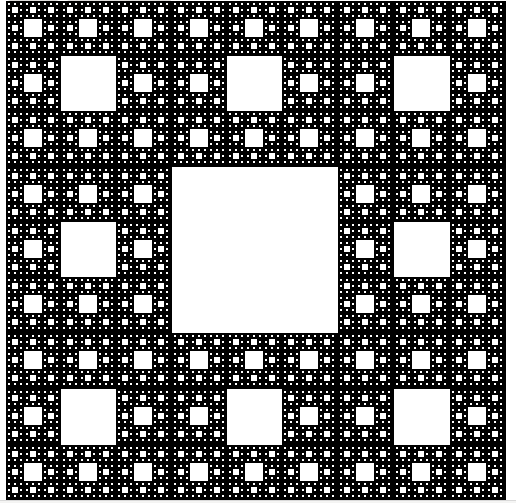
\includegraphics[width=7cm]{tapis.png}
\label{tapis_rec}
\end{figure}

Largement similaire au triangle, on implémente le code \ref{code_tapis_rec} (méthode récursive).

\begin{table}[H]
\caption{Tapis de Sierpinski (méthode récursive)}
\begin{tabular}{l}
\lstinputlisting[language=scilab]{tapis_sierpinski_recursif.sce}\\
\end{tabular}
\label{code_tapis_rec}
\end{table}

L'exécution du code nous donne ainsi la figure \ref{tapis_rec}.
\begin{figure}[H]
\centering
\caption{Tapis de Sierpinski (récursif) pour n=2}
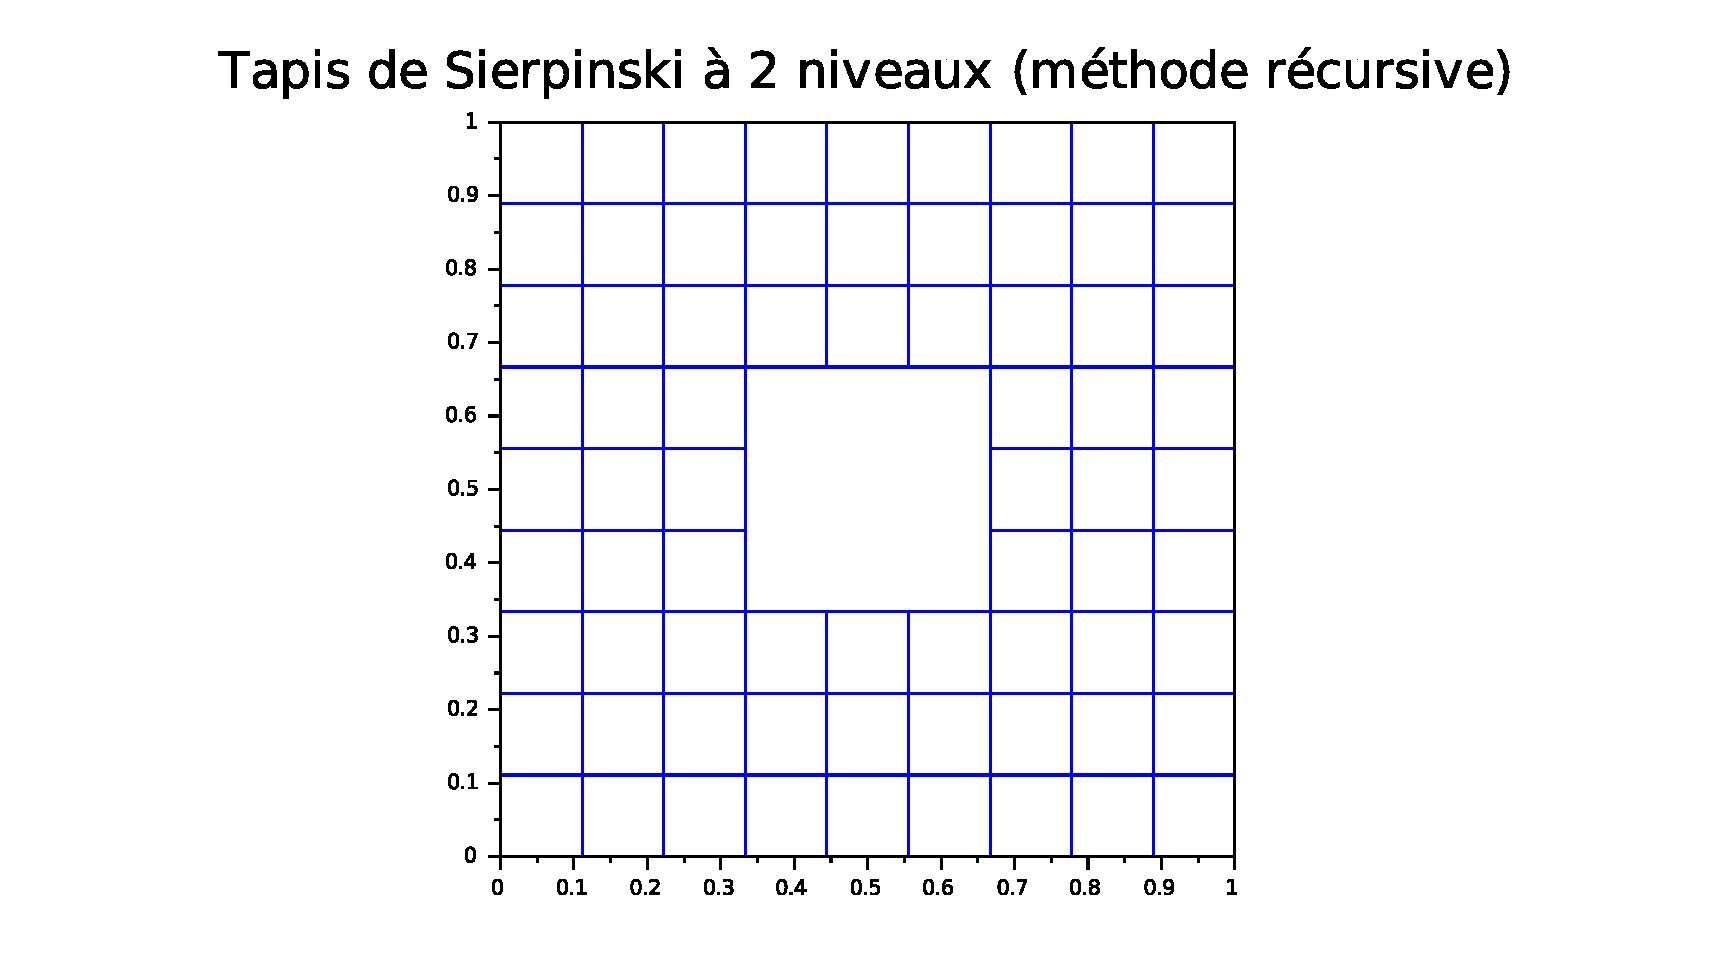
\includegraphics[width=0.75\textwidth]{tapis_recursif.pdf}
\label{tapis_rec}
\end{figure}

\newpage
On obtient donc un algorithme récursif de complexité en $O(8^n)$, complexité difficilement supportable pour la machine (mon ordinateur ne parvient à dessiner dans un temps raisonnable que le niveau $n=2$...). On implémente donc également la méthode itérative avec le code \ref{code_tapis_it} suivant l'IFS :

\begin{equation}
\left\lbrace
\begin{array}{lll}
f_1 \left[ \begin{array}{l} x \\ y \end{array} \right] =
\left[ \begin{array}{ll} \frac{1}{3} & 0 \\ 0 & \frac{1}{3} \end{array} \right]
\left[ \begin{array}{l} x \\ y \end{array} \right]
& &
f_2 \left[ \begin{array}{l} x \\ y \end{array} \right] =
\left[ \begin{array}{ll} \frac{1}{3} & 0 \\ 0 & \frac{1}{3} \end{array} \right]
\left[ \begin{array}{l} x \\ y \end{array} \right]
+ \left[ \begin{array}{l} \frac{1}{3} \\ 0 \end{array} \right]\\ \\

f_3 \left[ \begin{array}{l} x \\ y \end{array} \right] =
\left[ \begin{array}{ll} \frac{1}{3} & 0 \\ 0 & \frac{1}{3} \end{array} \right]
\left[ \begin{array}{l} x \\ y \end{array} \right]
+ 2 \times \left[ \begin{array}{l} \frac{1}{3} \\ 0 \end{array} \right]
& &
f_4 \left[ \begin{array}{l} x \\ y \end{array} \right] =
\left[ \begin{array}{ll} \frac{1}{3} & 0 \\ 0 & \frac{1}{3} \end{array} \right]
\left[ \begin{array}{l} x \\ y \end{array} \right]
+ \left[ \begin{array}{l} 0 \\ \frac{1}{3} \end{array} \right]\\ \\

f_5 \left[ \begin{array}{l} x \\ y \end{array} \right] =
\left[ \begin{array}{ll} \frac{1}{3} & 0 \\ 0 & \frac{1}{3} \end{array} \right]
\left[ \begin{array}{l} x \\ y \end{array} \right]
+ 2 \times \left[ \begin{array}{l} \frac{1}{3} \\ 0 \end{array} \right] + \left[ \begin{array}{l} 0 \\ \frac{1}{3} \end{array} \right]
& &
f_6 \left[ \begin{array}{l} x \\ y \end{array} \right] =
\left[ \begin{array}{ll} \frac{1}{3} & 0 \\ 0 & \frac{1}{3} \end{array} \right]
\left[ \begin{array}{l} x \\ y \end{array} \right]
+ \left[ \begin{array}{l} \frac{1}{3} \\ 0 \end{array} \right]\\ \\

f_7 \left[ \begin{array}{l} x \\ y \end{array} \right] =
\left[ \begin{array}{ll} \frac{1}{3} & 0 \\ 0 & \frac{1}{3} \end{array} \right]
\left[ \begin{array}{l} x \\ y \end{array} \right]
+ \left[ \begin{array}{l} \frac{1}{3} \\ 0 \end{array} \right] + 2 \times \left[ \begin{array}{l} 0 \\ \frac{1}{3} \end{array} \right] & &\\ \\
f_8 \left[ \begin{array}{l} x \\ y \end{array} \right] =
\left[ \begin{array}{ll} \frac{1}{3} & 0 \\ 0 & \frac{1}{3} \end{array} \right]
\left[ \begin{array}{l} x \\ y \end{array} \right]
+ 2 \times \left[ \begin{array}{l} \frac{1}{3} \\ 0 \end{array} \right] + 2 \times \left[ \begin{array}{l} 0 \\ \frac{1}{3} \end{array} \right]
\end{array}\right.
\end{equation}

\begin{table}[H]
\caption{Tapis de Sierpinski (méthode itérative)}
\begin{tabular}{l}
\lstinputlisting[language=scilab]{tapis_sierpinski_recursif.sce}\\
\end{tabular}
\label{code_tapis_it}
\end{table}

L'exécution du code nous donne ainsi la figure \ref{tapis_it}.
\begin{figure}[H]
\centering
\caption{Tapis de Sierpinski (itératif) pour n=100000 points}
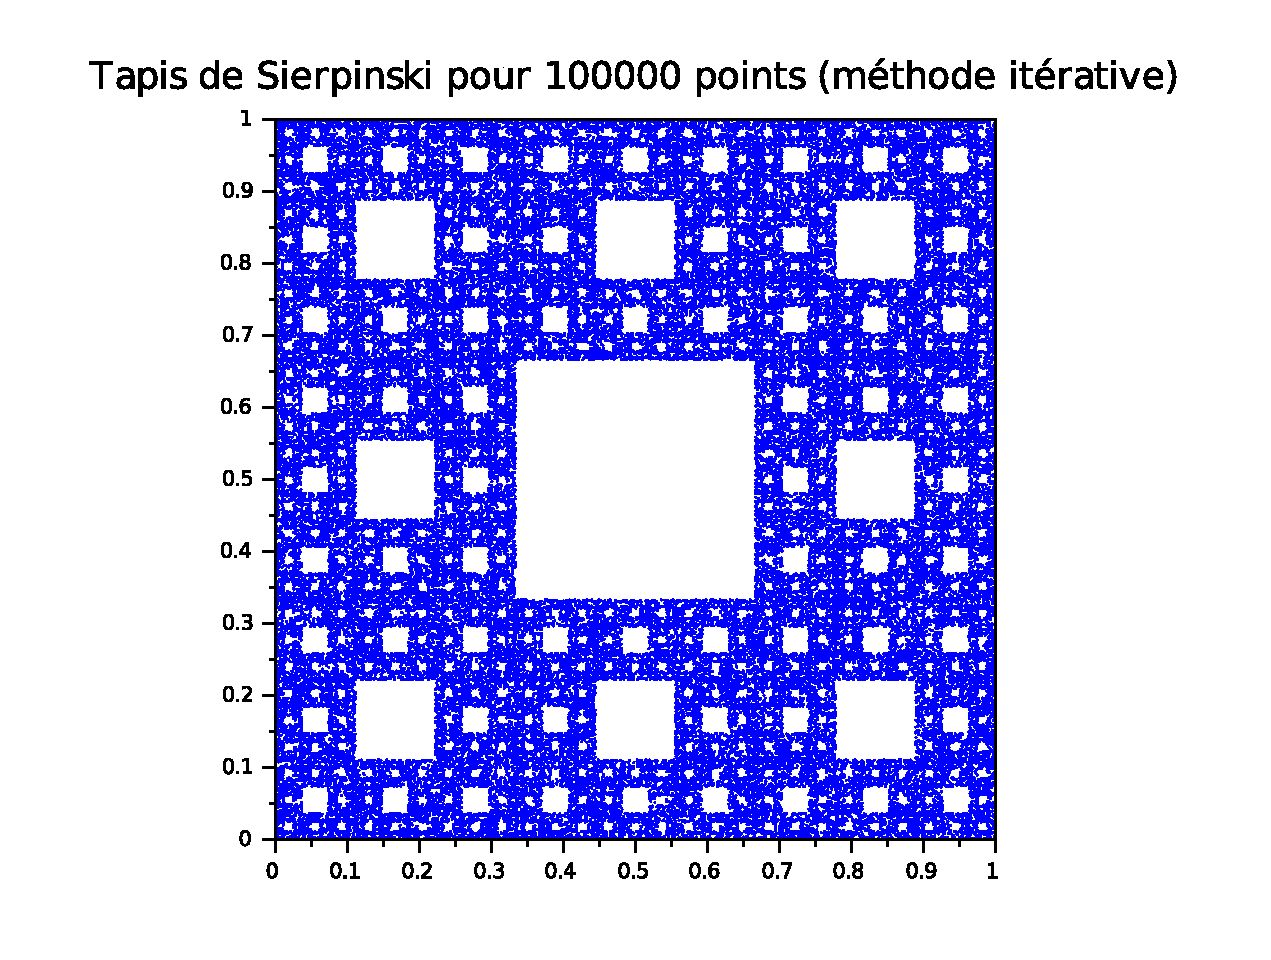
\includegraphics[width=0.75\textwidth]{tapis_iteratif.pdf}
\label{tapis_it}
\end{figure}


\section{Flocon de neige de Von Koch}
\subsection{Théorie}
\subsubsection{Présentation}
\begin{minipage}[c]{.70\linewidth}
	\indent Notre analyse continue avec l'étude d'une troisième fractale construite par Helge Von Koch, mathématicien suédois, fractale nommée le \textit{flocon de Von Koch}.
	\begin{figure}[H]
	\centering
	\caption{Flocon de neige de Von Koch}
	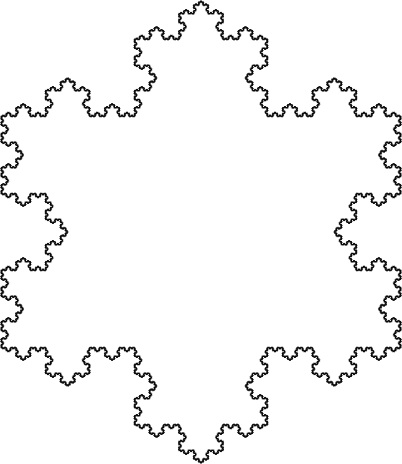
\includegraphics[width=6cm]{koch.jpg}
	\end{figure}
\end{minipage} \hfill
\begin{minipage}[c]{.05\linewidth}
\end{minipage} \hfill
\begin{minipage}[c]{.21\linewidth}
	\begin{figure}[H]
	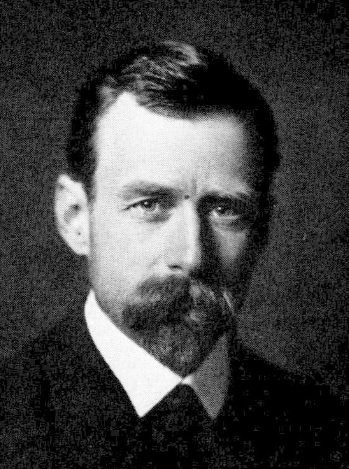
\includegraphics[height=4cm]{mr_koch.png}
	\caption{Von Koch 1870-1924}
	\end{figure}
\end{minipage}

\newpage
\subsubsection{Définition algorithmique}
\begin{algorithm}
\begin{algorithmic}
\REQUIRE{Un triangle équilatéral de côté 1}
\STATE \textbf{Opération de base :} Chaque segment du triangle est partagé en 3 parties égales.\\
Le segment central $S_C$ est remplacé par 2 segments égaux formant un triangle équilatéral ayant pour base $S_C$
\STATE \textbf{Itération :} Itérer l'opération sur chacun des segments obtenus
\end{algorithmic}
\end{algorithm}

\subsubsection{Remarques}
A l'infini, on obtient donc $\mathsf{K^{(\infty)}}$ le flocon de Van Koch. On a en outre les propriétés suivantes :\\
\begin{align*}
   i) \ & l(\mathsf{K^{(\infty)}})=+\infty \\
   ii) \ & \mathit{A}(\mathsf{K^{(\infty)}})<\infty
\end{align*}
En effet :\\
\textbf{longueur :}\\
\begin{tabular}{cccccc}
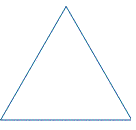
\includegraphics[height=2cm]{koch_l0.png} & $\rightarrow$ & 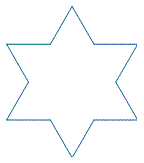
\includegraphics[height=2cm]{koch_l1.png} & $\rightarrow$ & 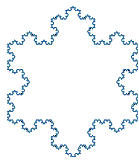
\includegraphics[height=2cm]{koch_k.png} &\\
$l_0=3$ & & $l_1=12\times \frac{1}{3}=4$ & ... & $l_k=4^k$ & $\overset{k \rightarrow +\infty}{\longrightarrow} +\infty $\\
\end{tabular} \\ \\ \\
\textbf{aire :}\\
\begin{tabular}{ccccc}
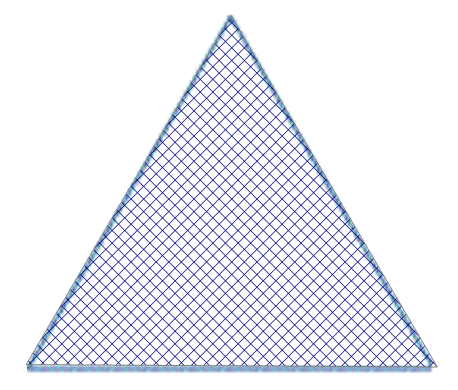
\includegraphics[height=2cm]{koch_a0.png} & $\rightarrow$ & 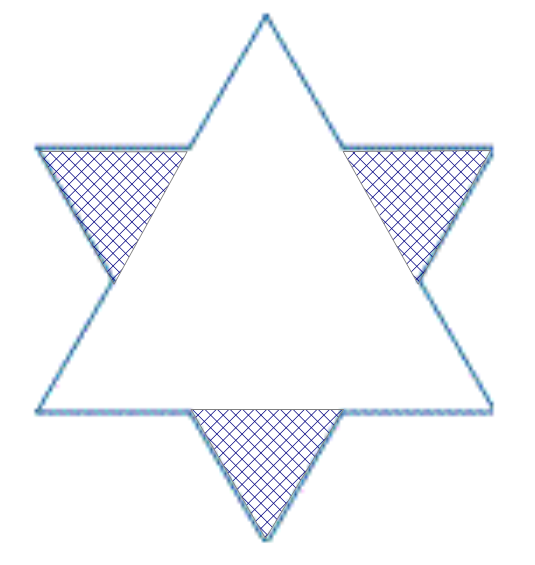
\includegraphics[height=2cm]{koch_a1.png} & $\rightarrow$ & 
$
\left\lbrace
\begin{array}{l}
A_2 = A_1 + \frac{12A_0}{3^4}=A_1+\frac{2^2}{3^3}A_0 \\
\\
A_3 = A_2 + \frac{48A_0}{3^6}=A_1+\frac{2^4}{3^5}A_0
\end{array}\right.
 $\\
$A_0$ & & $A_1=A_0 + \frac{3A_0}{9}$ & & \\
&&$=A_0 + \frac{A_0}{3}$&&\\
\end{tabular} \\ \\ \\
donc $A_k=A_0+A_0\frac{1}{3}+A_0\frac{2^2}{3^3}+A_0\frac{2^4}{3^5}+\cdots + A_0\frac{2^{2k}}{3^{2k+1}}$\\
à l'infini, on a donc : $A_{\infty}=A_0+ \sum \limits_{k=0}^\infty \frac{2^{2k}}{3^{2k+1}} = A_0 + \frac{A_0}{3}\sum \limits_{k=0}^\infty \left( \frac{2}{3} \right)^{2k}$ = ?

\subsubsection{Dimension du Flocon de Von Koch}
On applique donc la définition de la dimension de Hausdorff au flocon de Von Koch :\\ \\
\begin{tabular}{ccccc}
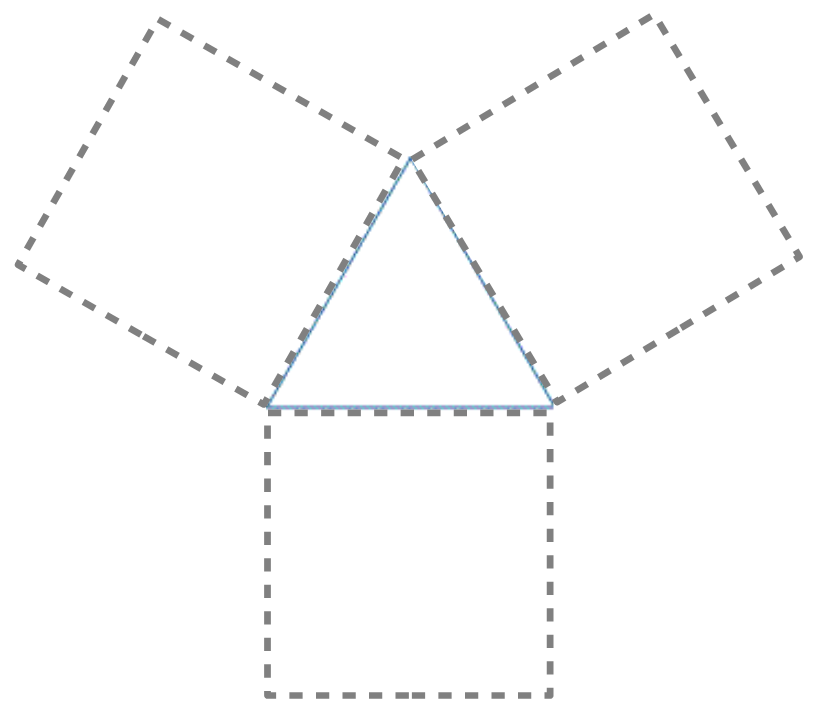
\includegraphics[height=2.4cm]{koch_0.png} & $\rightarrow$ & 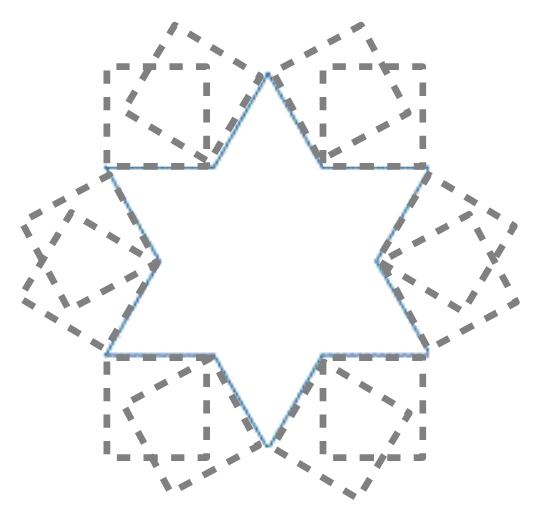
\includegraphics[height=2.5cm]{koch_1.png} & $\rightarrow$ & 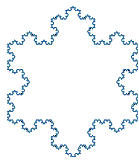
\includegraphics[height=2.5cm]{koch_k.png}\\
$K^{(0)}$ & & $K^{(1)}$ & ... & $K^{(k)}$\\
1 seul carré & & 12 carrés & ... & $3\times 4^k$ carrés\\
de côté 1 & & de côté $\frac{1}{3}$ & ... & de côté $\varepsilon_k = \frac{1}{3^k}$\\
\end{tabular} \\ \\ \\
Donc $d=\lim\limits_{k \rightarrow \infty} 3\times \frac{ln(4^k)}{ln(3^k)}=3\times \frac{ln(4)}{ln(3)}=3\times \frac{2ln(2)}{ln(3)}$ est la dimension de Hausdorff.\\ \\
On peut restreindre l'étude du flocon de Von Koch à l'étude de la courbe de Von Koch (figure \ref{courbe_vonkoch}). L'algorithme de construction est le même à l'exception que la figure de départ est un segment et non un triangle. On a alors $d=\frac{2ln(2)}{ln(3)}$.
\begin{figure}[H]
\caption{Courbe de Von Koch}
\label{courbe_vonkoch}
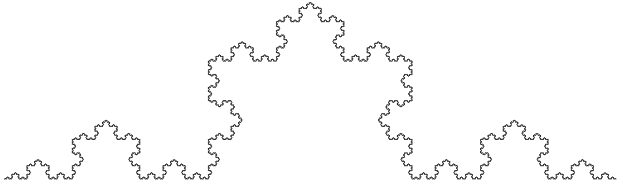
\includegraphics[width=\textwidth]{koch_courbe.png}
\end{figure}

Dans nos applications dans \textit{Scilab}, on se contentera de tracer la courbe de Von Koch. \\ \\

\subsection{Application dans \textit{Scilab} (méthode récursive)}
En s'insipirant toujours de la définition de la fractale, on implémente dans \textit{Scilab} le code \ref{code_koch}.
\begin{table}[H]
\caption{Courbe de Von Koch (méthode récursive)}
\begin{tabular}{l}
\lstinputlisting[language=scilab]{koch_recursif.sce}\\
\end{tabular}
\label{code_koch}
\end{table}
\newpage
L'exécution du code nous donne ainsi la figure \ref{koch_recursif}.
\begin{figure}[H]
\centering
\caption{Figure pour n=4}
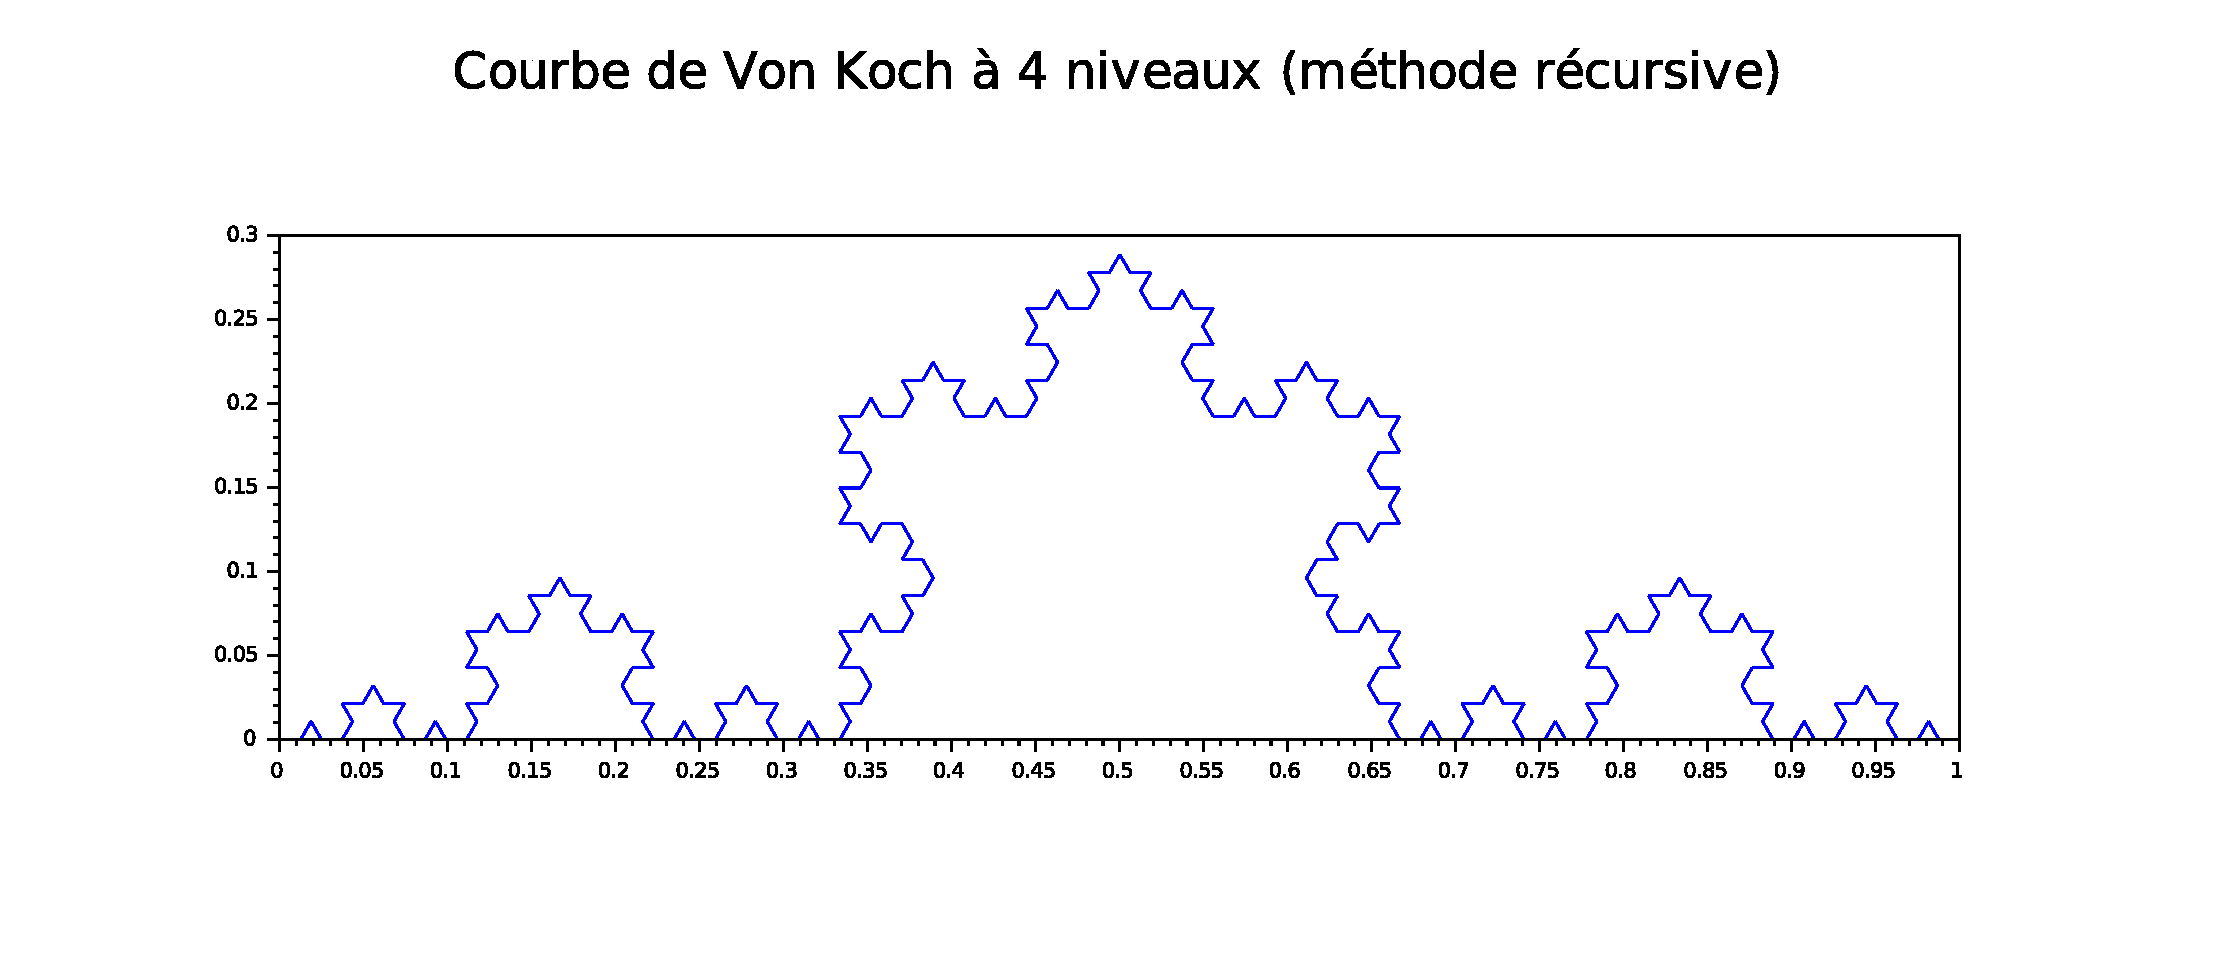
\includegraphics[width=\textwidth]{koch_recursif.pdf}
\label{koch_recursif}
\end{figure}

\subsection{Application dans \textit{Scilab} (méthode itérative)}
La complexité de l'algorithme récursif est ici en $O(4^n)$ (on réalise 4 appels récursifs pour chaque niveau). L'éxecution devient donc très rapidement problématique. Pour des valeurs de $n$ importantes, cette méthode n'est plus applicable. On implémente donc également une méthode itérative à l'aide d'un IFS. On a donc :
\begin{equation}
\left\lbrace
\begin{array}{l}
f_1 \left[ \begin{array}{l} x \\ y \end{array} \right] =
\left[ \begin{array}{ll} \frac{1}{3} & 0 \\ 0 & \frac{1}{3} \end{array} \right]
\left[ \begin{array}{l} x \\ y \end{array} \right]\\ \\

f_2 \left[ \begin{array}{l} x \\ y \end{array} \right] =
\left[ \begin{array}{ll} \frac{1}{6} & -\frac{\sqrt{3}}{6} \\ \frac{\sqrt{3}}{6} & \frac{1}{6} \end{array} \right]
\left[ \begin{array}{ll} x \\ y \end{array} \right]
+ \left[ \begin{array}{l} \frac{1}{3} \\ 0 \end{array} \right]\\ \\

f_3 \left[ \begin{array}{l} x \\ y \end{array} \right] \longrightarrow
\left[ \begin{array}{ll} \frac{1}{6} & \frac{\sqrt{3}}{6} \\ -\frac{\sqrt{3}}{6} & \frac{1}{6} \end{array} \right]
\left[ \begin{array}{ll} x \\ y \end{array} \right]
+ \left[ \begin{array}{l} \frac{1}{2} \\ \frac{\sqrt{3}}{6} \end{array} \right]\\ \\

f_4 \left[ \begin{array}{l} x \\ y \end{array} \right] \longrightarrow
\left[ \begin{array}{ll} \frac{1}{3} & 0 \\ 0 & \frac{1}{3} \end{array} \right]
\left[ \begin{array}{ll} x \\ y \end{array} \right]
+ \left[ \begin{array}{l} \frac{2}{3} \\ 0 \end{array} \right]\\
\end{array}\right.
\end{equation}
$d'o\grave{u} \
\left\lbrace
\begin{array}{l}
K_0 \ donn\acute{e} \\
K_{n+1} = K(T_n) \ avec \ K(T)=f_0(T)\cup f_1(T)\cup f_2(T)\cup f_3(T)\cup f_4(T)\\
\end{array}\right.$\\ \\
Finalement $K_n$ converge au sens de la distance de Hausdorff vers $K^\infty$, le flocon de Von Koch. A nouveau, la dispersion des points doit être uniforme, on utilise donc des conditions d'équiprobabilité. \\ \\

\indent On implémente donc dans \textit{Scilab} le code \ref{code_koch_it}.
\begin{table}[H]
\caption{Flocon de Von Koch (méthode itérative)}
\begin{tabular}{l}
\lstinputlisting[language=scilab]{koch_iteratif.sce}\\
\end{tabular}
\label{code_koch_it}
\end{table}

L'exécution du code nous donne ainsi la figure \ref{koch_iteratif}.
\begin{figure}[H]
\centering
\caption{Flocon de Von Koch itératif pour 10000 points}
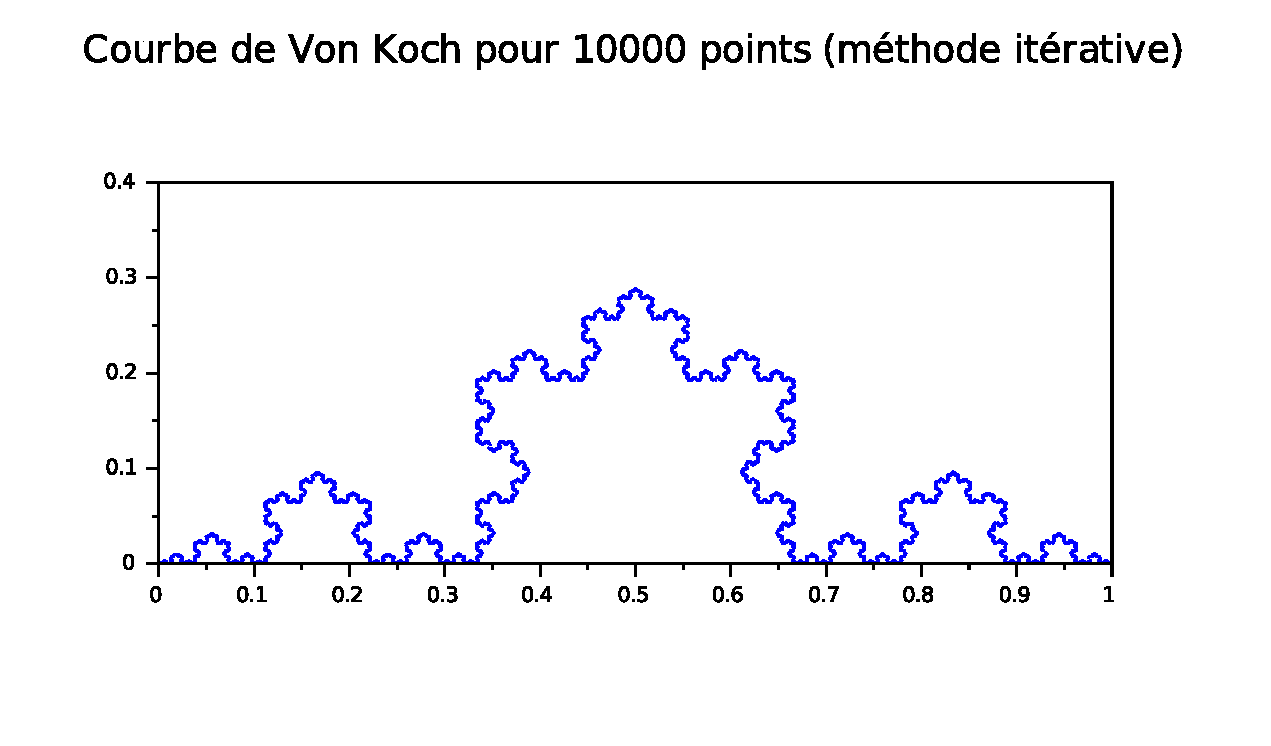
\includegraphics[width=\textwidth]{koch_iteratif.pdf}
\label{koch_iteratif}
\end{figure}

\newpage
\section{Fougère de Barnsley}
\subsection{Théorie}
\subsubsection{Présentation}
\begin{minipage}[c]{.70\linewidth}
	\indent Pour compléter notre étude sur la théorie des IFS, on va s'intéresser à un objet qu'il est impossible de construire de manière récursive : la \textit{fougère de Barnsley}, construite par Michael Barnsley, mathématicien britannique. \\ \\
	On a précédemment vu trois applications de la méthode des IFS avec à chaque fois une dispersion des points de manière uniforme. Il apparaît donc pertinent de s'intéresser à une fractale nécessitant une certaine dispersion des points : \textit{la fougère de Barnsley}.
\end{minipage} \hfill
\begin{minipage}[c]{.05\linewidth}
\end{minipage} \hfill
\begin{minipage}[c]{.21\linewidth}
	\begin{figure}[H]
	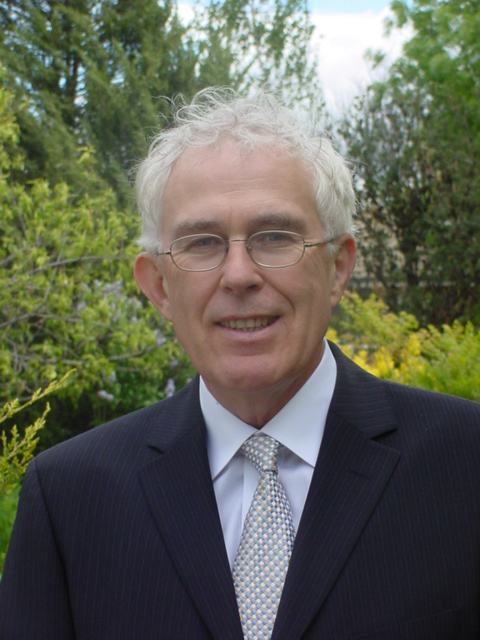
\includegraphics[height=4cm]{mr_barnsley.jpg}
	\caption{Barnsley 1946-...}
	\end{figure}
\end{minipage}

\begin{figure}[H]
\centering
\caption{Fougère de Barnsley}
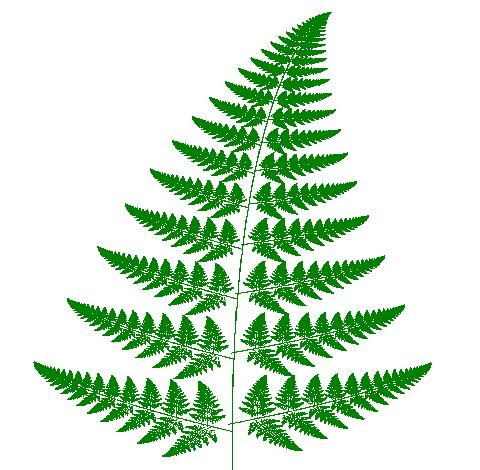
\includegraphics[width=5.5cm]{barnsley.jpg}
\end{figure}

\subsubsection{Définition}
Le système de fonctions itérées est le suivant :
\begin{equation}
\left\lbrace
\begin{array}{l}
f_1\left[ \begin{array}{c} x \\ y \end{array} \right]\ = \ \left[ \begin{array}{cc} 0,00 & 0,00 \\ 0,00 & 0,16 \end{array} \right] \left[ \begin{array}{c} x \\ y \end{array} \right]\\
\\
f_2\left[ \begin{array}{c} x \\ y \end{array} \right]\ = \ \left[ \begin{array}{cc} 0,85 & 0,04 \\ -0,04 & 0,85 \end{array} \right] \left[ \begin{array}{c} x \\ y \end{array} \right] + \left[ \begin{array}{l} 0 \\ 1,6 \end{array} \right] \\
\\
f_3\left[ \begin{array}{c} x \\ y \end{array} \right]\ = \ \left[ \begin{array}{cc} 0,20 & -0,26 \\ 0,23 & 0,22 \end{array} \right] \left[ \begin{array}{c} x \\ y \end{array} \right] + \left[ \begin{array}{l} 0 \\ 1,6 \end{array} \right] \\
\\
f_3\left[ \begin{array}{c} x \\ y \end{array} \right]\ = \ \left[ \begin{array}{cc} 0,15 & 0,28 \\ 0,26 & 0,24 \end{array} \right] \left[ \begin{array}{c} x \\ y \end{array} \right] + \left[ \begin{array}{l} 0 \\ 0,44 \end{array} \right] \\
\end{array}\right.
\end{equation}
Ces fonctions sont responsables de la modélisation de chacune des parties de la fougère. Pour obtenir un dessin réaliste, il est donc nécessaire de privilégier certaines parties par rapport à d'autres (plus la partie gauche que le reste par exemple). \\
Il est conseillé de choisir les pondérations $p_i$ suivantes pour chacune des fonctions $f_i$ :
$p = \left[ \begin{array}{l} 0,01 \\ 0,85 \\ 0,07 \\ 0,07 \end{array} \right]$

\newpage
\subsection{Application dans \textit{Scilab}}
On implémente donc dans \textit{Scilab} le code \ref{code_fougere}.

\begin{table}[H]
\caption{Fougère de Barnsley}
\begin{tabular}{l}
\lstinputlisting[language=scilab]{fougere.sce}\\
\end{tabular}
\label{code_fougere}
\end{table}

L'exécution du code nous donne ainsi la figure \ref{affichage_fougere} pour différentes valeurs de $N$.
\begin{figure}[H]
\caption{Différents affichages de la fougère en fonction de $N$}
   \begin{minipage}[c]{.49\linewidth}
   \centering
      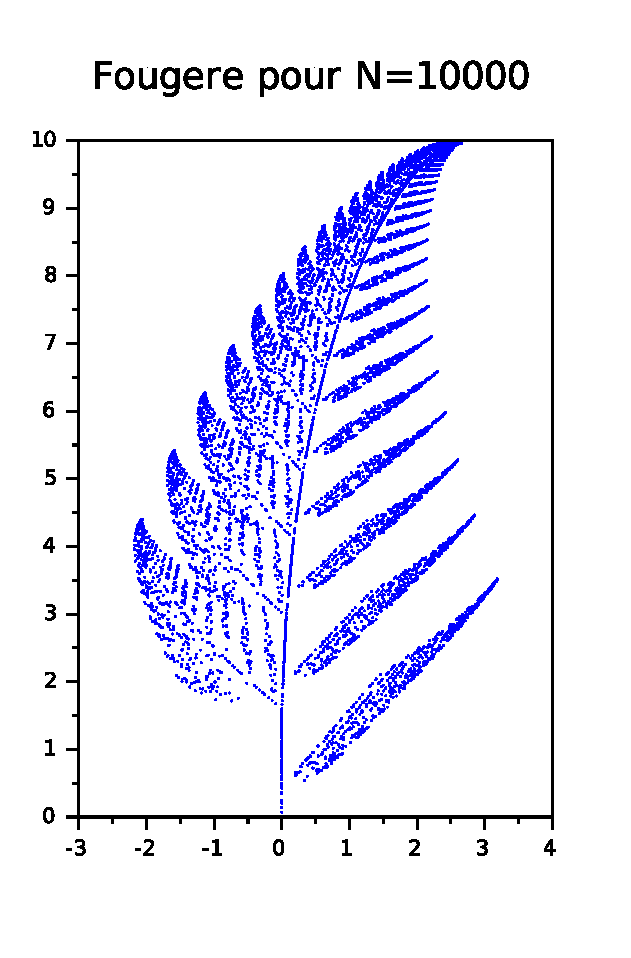
\includegraphics[height=8cm]{graphfougere.pdf}
   \end{minipage} \hfill
   \begin{minipage}[c]{.49\linewidth}
   \centering
      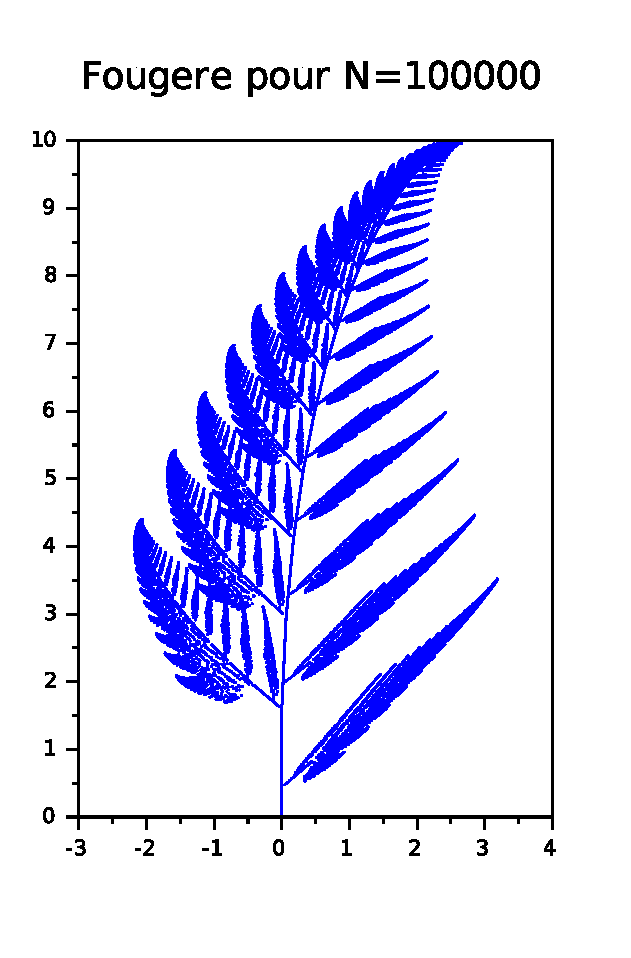
\includegraphics[height=8cm]{graphfougere_2.pdf}
   \end{minipage}
\label{affichage_fougere}
\end{figure}

\section{Ensemble de Julia}

\subsection{Théorie}
\subsubsection{Présentation}
\begin{minipage}[c]{.70\linewidth}
	\indent Nous allons maintenant nous intéresser à des fractales dont la construction est beaucoup moins immédiate que les précédentes (fractales dont on pouvait rapidement représenter quelques itérations, même avec un crayon et une feuille de papier). \\ \\
	La première de ces fractales \textit{plus compliquées} s'appelle l'ensemble de Julia, construite par Gaston Julia, un mathématicien français. Il est à noter que la figure \ref{julia} n'est pas représentative de l'ensemble de Julia : ce dernier peut prendre des formes très différentes selon la modélisation choisie et surtout selon la valeur de $c$. 
\end{minipage} \hfill
\begin{minipage}[c]{.05\linewidth}
\end{minipage} \hfill
\begin{minipage}[c]{.21\linewidth}
	\begin{figure}[H]
	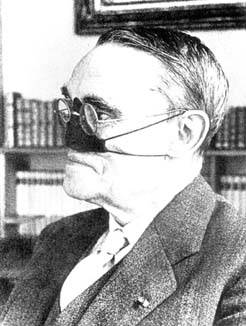
\includegraphics[height=4cm]{mr_julia.jpg}
	\caption{Julia 1893-1978}
	\end{figure}
\end{minipage}

\begin{figure}[H]
\centering
\caption{Ensemble de Julia (exemple parmi beaucoup d'autres)}
\label{julia}
\centering
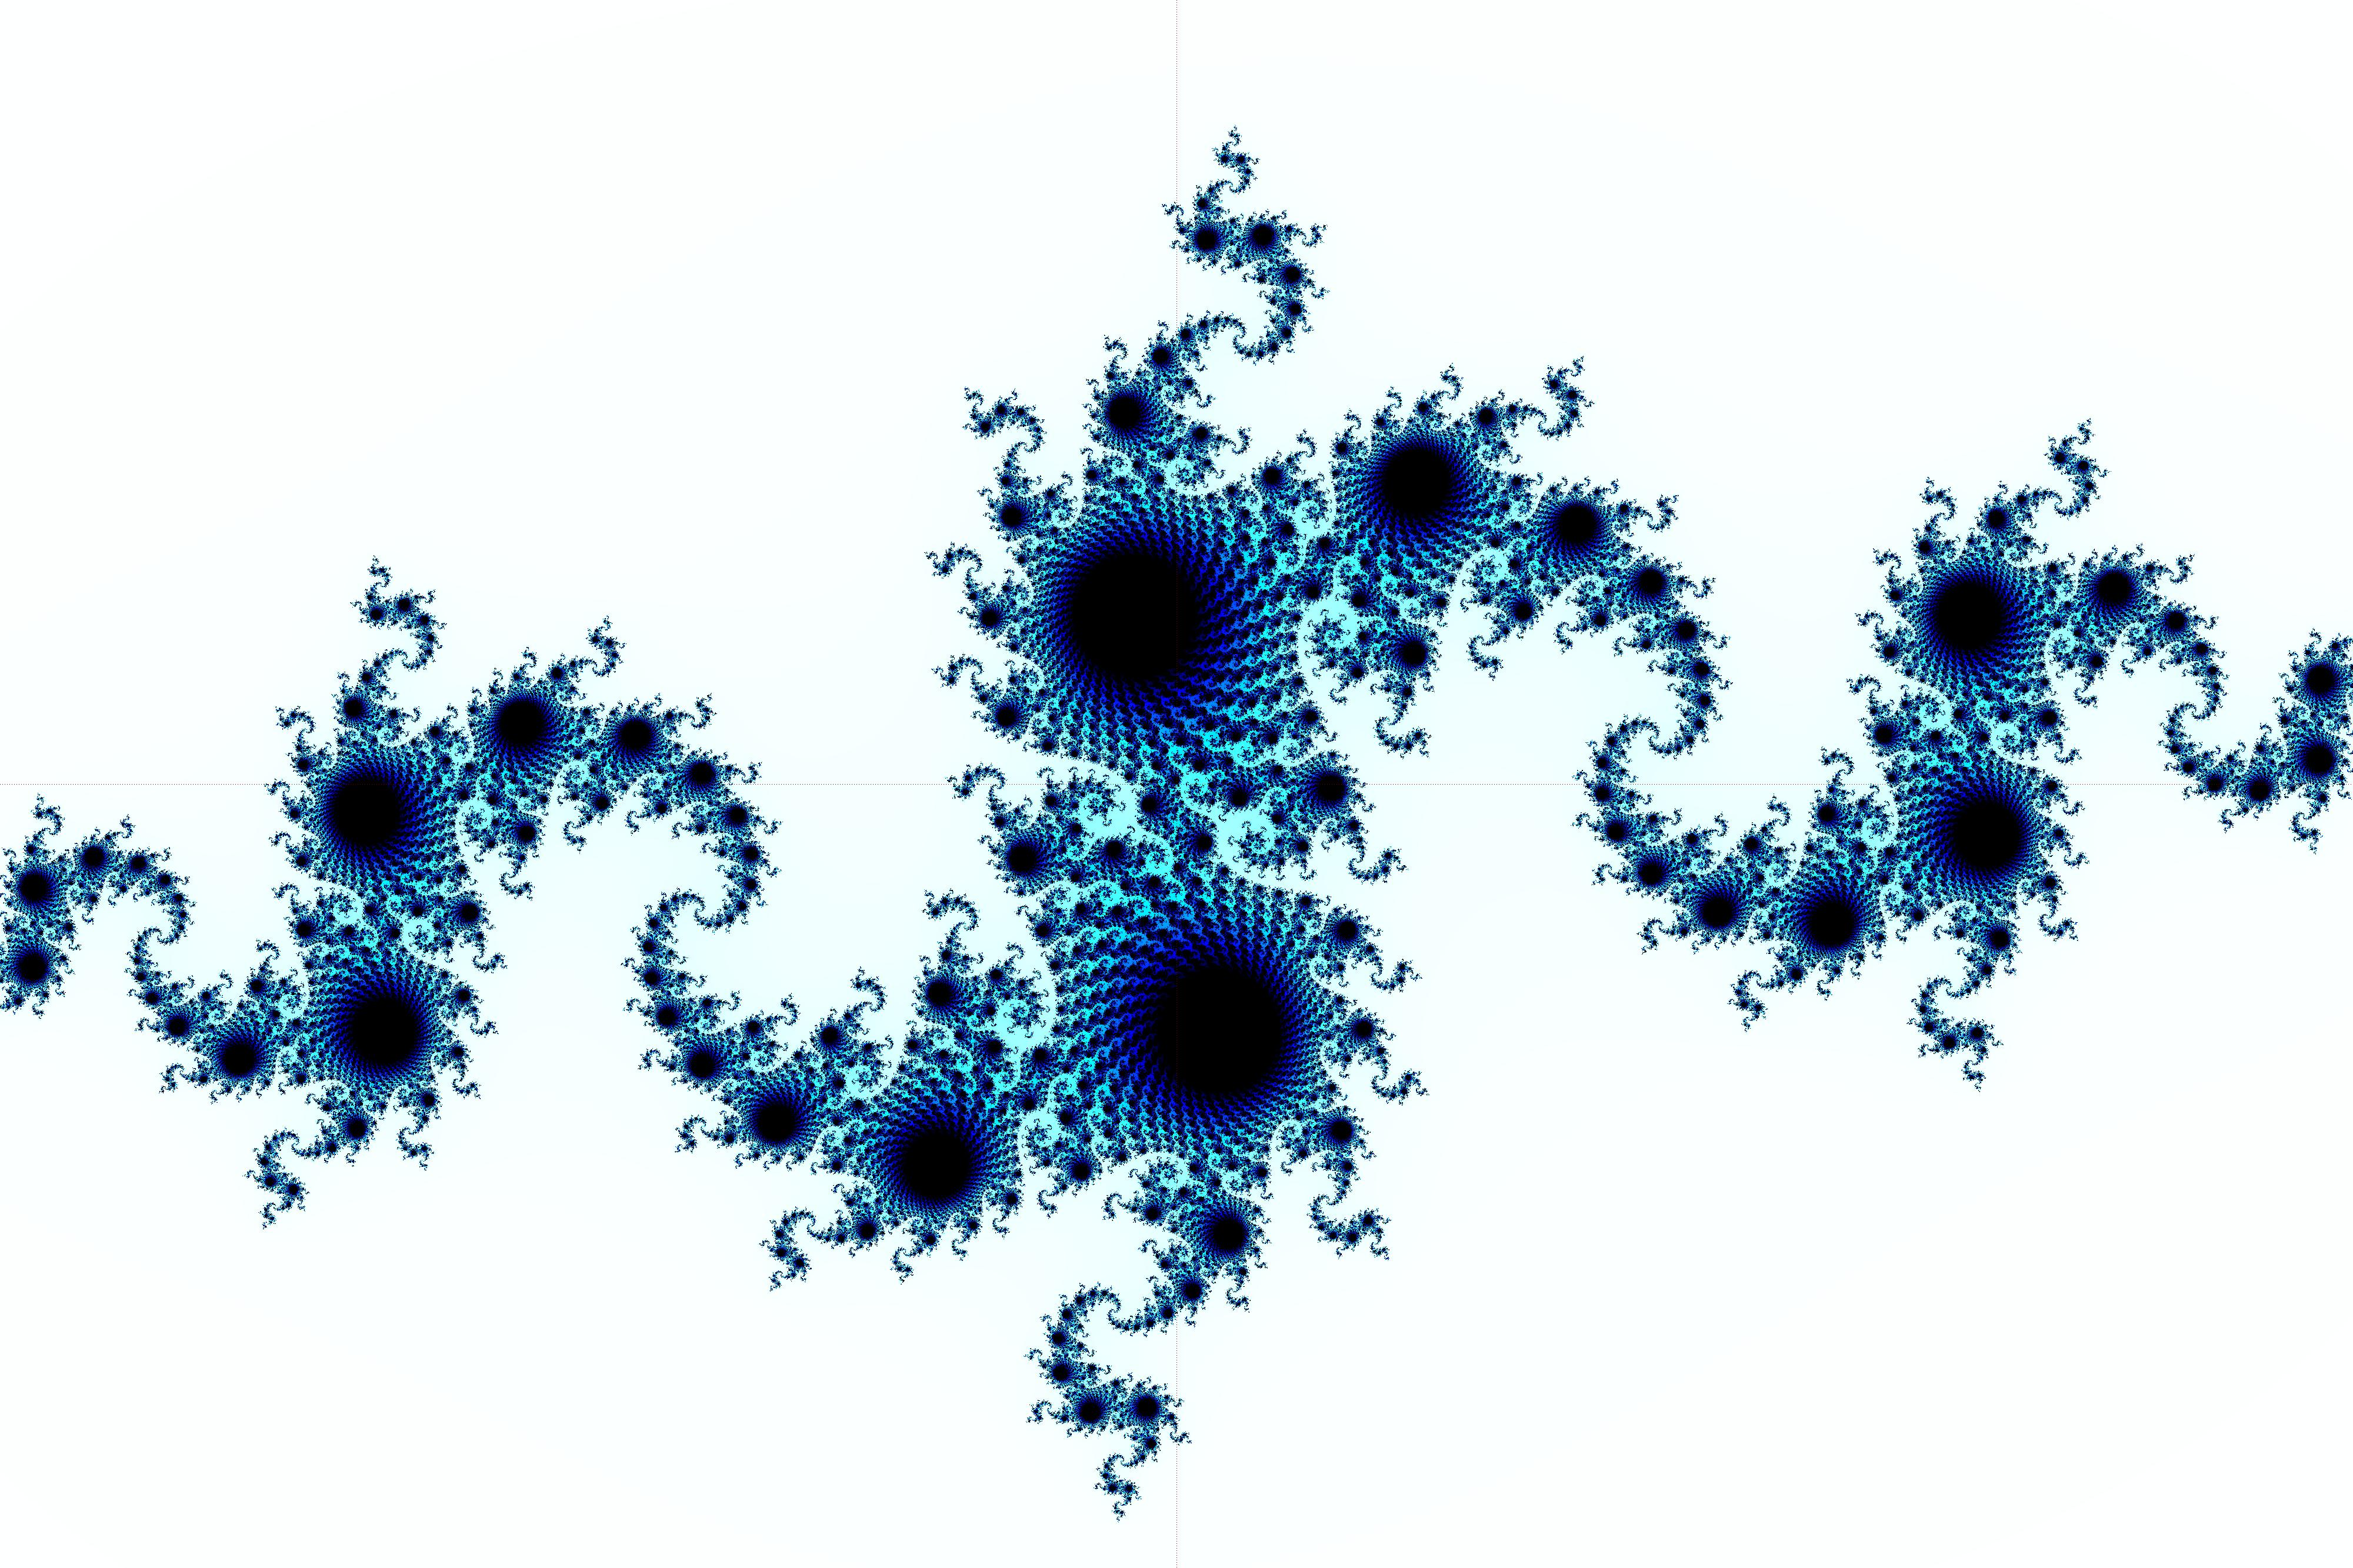
\includegraphics[width=14cm]{julia.jpg}
\end{figure}

\subsubsection{Définition}
On se donne un nombre complexe $c=a+ib$ avec $a,b\ \in \ \mathbb{R}$. On considère alors la suite :
\begin{equation}
\label{suite_julia}
\left\lbrace
\begin{array}{l}
z_{n+1}=z_n^2+c \\
z_0 \ \in \ \mathbb{C}
\end{array}\right.
\end{equation}
On appelle \textit{bassin d'attraction} l'ensemble des points $z_0$ tels que la suite définie en (\ref{suite_julia}) converge, et \textit{bassin de répulsion} l'ensemble des points $z_0$ tels que la suite diverge. L'ensemble de Julia est alors la frontière entre ces deux bassins. L'ensemble de Julia est alors défini en fonction de $c$, qui en devient un paramètre capital. Le choix de $c$ est classique et on peut trouver beaucoup de documentation en ligne sur les valeurs intéressantes à donner à cette variable. En outre, nous verrons un peu plus tard que ces valeurs ne sont pas le fruit du hasard.

\subsection{Application dans \textit{Scilab}}
On implémente donc dans \textit{Scilab} le code \ref{code_julia}.

\begin{table}[H]
\caption{Ensemble de Julia}
\begin{tabular}{l}
\lstinputlisting[language=scilab]{julia.sce}\\
\end{tabular}
\label{code_julia}
\end{table}

L'exécution du code nous donne ainsi la figure \ref{affichage_julia} pour différentes valeurs de $c$.
\begin{figure}[H]
\caption{Différents affichages de l'ensemble de Julia en fonction de $c$}
   \begin{minipage}[c]{.49\linewidth}
   \centering
      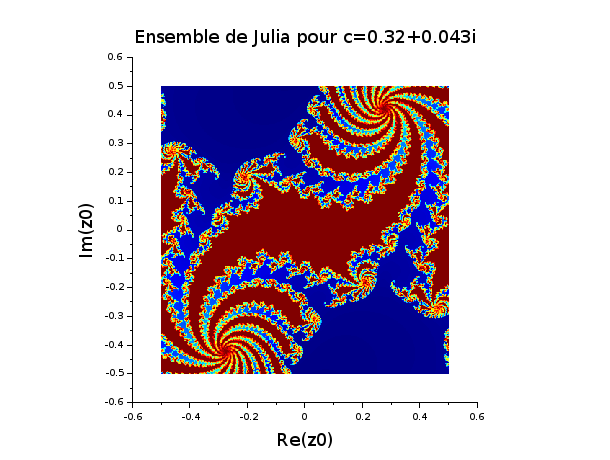
\includegraphics[height=6.5cm]{julia1.png}
      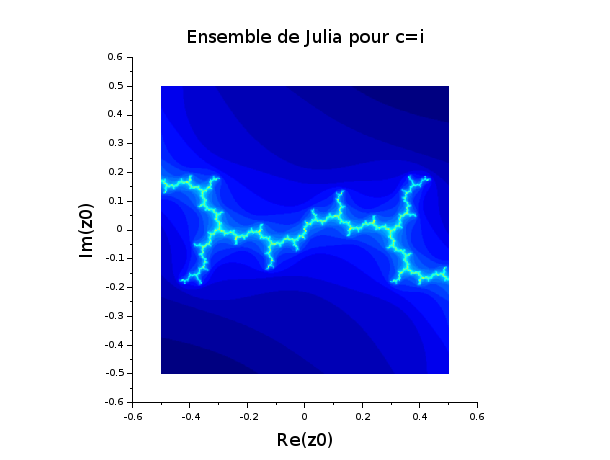
\includegraphics[height=6.5cm]{julia2.png}
   \end{minipage} \hfill
   \begin{minipage}[c]{.49\linewidth}
   \centering
      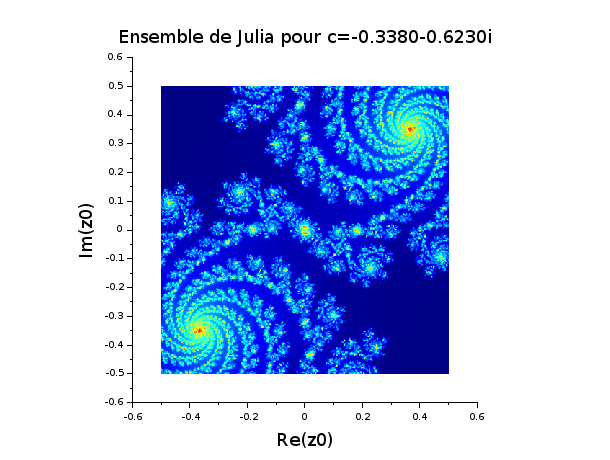
\includegraphics[height=6.5cm]{julia3.png}
      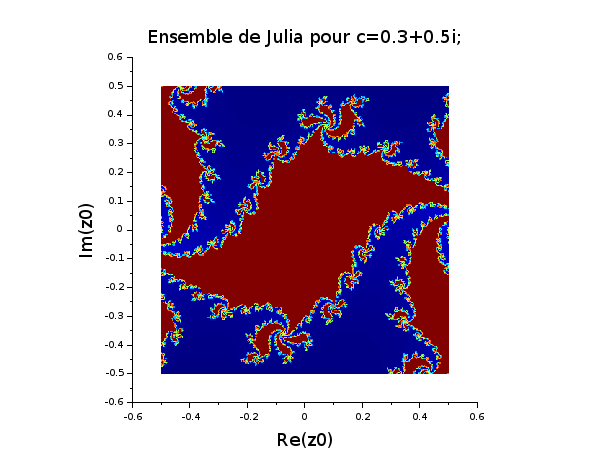
\includegraphics[height=6.5cm]{julia4.png}
   \end{minipage}
\label{affichage_julia}
\end{figure}


\section{Ensemble de Mandelbrot}
\subsection{Théorie}
\subsubsection{Présentation}
Avec l'ensemble de Julia, nous avions vu que la sélection d'une valeur de $c$ \textit{intéressante} était primordiale à la construction de la fractale. \\ \\
\begin{minipage}[c]{.70\linewidth}
	Ainsi la fractale que nous sommes sur le point d'étudier nous permet une représentation de ces valeurs de $c$ en fonction de leur \textit{intérêt}. Il s'agit donc de la fractale nommée \textit{l'ensemble de Mandelbrot}, construite par Benoît Mandelbrot, mathématicien franco-américain.
\begin{figure}[H]
\centering
\caption{Ensemble de Mandelbrot}
\label{julia}
\centering
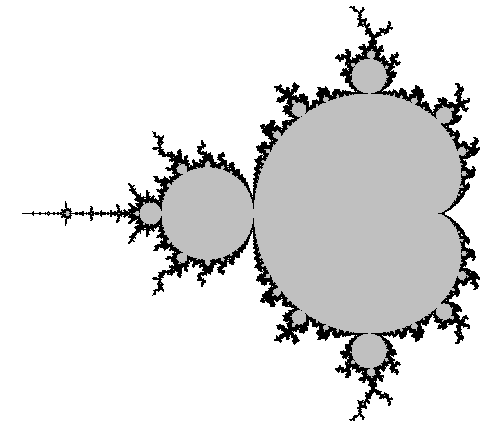
\includegraphics[width=6cm]{mandelbrot.png}
\end{figure}	
\end{minipage} \hfill
\begin{minipage}[c]{.05\linewidth}
\end{minipage} \hfill
\begin{minipage}[c]{.21\linewidth}
	\begin{figure}[H]
	\includegraphics[height=4cm]{mr_mandelbrot.jpg}
	\caption{Mandelbrot 1924-2010}
	\end{figure}
\end{minipage}

\subsubsection{Définition}
La définition de l'ensemble de Mandelbrot est donc largement similaire à celle de l'ensemble de Julia, à la seule différence prés que la valeur de $z_0$ est donnée et que $c$ est une variable.

\subsection{Application dans \textit{Scilab}}
On implémente donc dans \textit{Scilab} le code \ref{code_mandelbrot}.

\begin{table}[H]
\caption{Ensemble de Mandelbrot}
\begin{tabular}{l}
\lstinputlisting[language=scilab]{mandelbrot.sce}\\
\end{tabular}
\label{code_mandelbrot}
\end{table}

L'exécution du code nous donne ainsi la figure \ref{affichage_mandelbrot}.
\begin{figure}[H]
\caption{Ensemble de Mandelbrot}
\centering
\includegraphics[height=8cm]{mandelbrot1.png}
\label{affichage_mandelbrot}
\end{figure}
Ainsi, en construisant les ensembles de Julia associés aux $c$ \textit{intéressants} (dans la limite entre les zones rouge et bleue), on obtient une figure connexe.\\
\indent En effet, on peut comparer les affichages de la figure \ref{affichage_julia_cf_mandelbrot}.

\begin{figure}[H]
\caption{Différents affichages de l'ensemble de Julia en fonction de $c$ (dans ou hors la frontière de Mandelbrot)}
   \begin{minipage}[c]{.49\linewidth}
   \centering
      \includegraphics[height=5.5cm]{julia1_cfM.png}
      \includegraphics[height=5.5cm]{julia2_cfM.png}
   \end{minipage} \hfill
   \begin{minipage}[c]{.49\linewidth}
   \centering
      \includegraphics[height=5.5cm]{julia3_cfM.png}
      \includegraphics[height=5.5cm]{julia4_cfM.png}
   \end{minipage}
\label{affichage_julia_cf_mandelbrot}
\end{figure}

\chapter{Équations différentielles}
\section{Introduction}
Dans de très nombreux domaines comme la mécanique, la biologie, la chimie ou encore l'économie, beaucoup de problèmes font appel à des équations différentielles. On est ainsi souvent confronté à ce que l'on appelle des \textit{problème de Cauchy} sous la forme suivante :\\
\begin{equation}
\label{equa_diff}
\left\lbrace
\begin{array}{l}
y^{(m)}=h(t,y,y',\cdots ,y^{(m-1)}) \\
y(0)=a_0 \\
y'(0)=a_1 \\
\cdots \\
y^{(m-1)}(0)=a_{m-1} \\
\end{array}\right.
\end{equation}

Pour résoudre (\ref{equa_diff}), on se ramène alors à un système différentiel d'ordre 1 :
\begin{equation}
\begin{array}{llllll}
Y= &
\left(
\begin{array}{l}
y_1 \ (la \ solution) \\
y_2=y'_1 \\
\vdots \\
y_m=f(t,y_1,y_2,\cdots ,y_{m-1}) \\
\end{array}\right)

& &
Y(0)= &
\left(
\begin{array}{c}
a_0 \\
a_1 \\
\vdots \\
a_{m-1} \\
\end{array}\right) \in \textbf{R}^m \\ \\
donc &
\left\lbrace
\begin{array}{l}
Y'=F(t,Y) \\
y(0)=(a_0,\cdots ,a_{m-1})^T \\
\end{array}\right.
& avec & F(t,Y)= &
\left(
\begin{array}{c}
y_1\\
y_2\\
\vdots \\
y_{m-1} \\
f(t,y_1,y_2,\cdots ,y_{m-1})
\end{array}\right)
\end{array}
\end{equation}
\\

\indent Cependant, considérons le problème suivant :
\begin{equation}
\label{equa_diff_pb}
\left\lbrace
\begin{array}{l}
y'=e^{-t^2}y \\
y(0)=1
\end{array}\right.
\end{equation}
on a (\ref{equa_diff_pb}) $\Rightarrow \ \frac{dy}{dt} = e^{-t^2}y \ \Rightarrow \ \frac{dy}{y} = e^{-t^2}dt \ \Rightarrow \ \int_{}^{} \frac{dy}{y} = \int_{}^{} e^{-t^2}dt \ \Rightarrow \ ln(y) = \int_{}^{} e^{-t^2}dt $\\
Or on ne connaît pas de primitive de $t \longrightarrow e^{-t^2}$, on ne peut donc pas résoudre le système (\ref{equa_diff_pb}) de manière analytique. Dans ce genre de situation, on a alors recours à un schéma numérique.

\newpage
\section{Idée, stabilité, consistance et ordre d'un schéma numérique}
\subsection{Idée}
L'idée générale d'un schéma numérique est la suivante :\\
On crée une subdivision de l'intervalle d'étude $[t_0,t_0+T]$.\\
On obtient donc $\sigma = \left\lbrace t_0,t_1,\cdots ,t_N \right\rbrace$ avec $t_N=t_0+N$.\\
On note le pas de la subdivision $h=\underset{0\leq i \leq N}{max} |t_{i+1}-t_i|$.\\
On se placera toujours dans la cas d'une substitution \textit{uniforme} : $h_i=|t_{i+1}-t_i|=h \ \ \ \forall i$\\
L'idée est alors d'approcher $y(t_i)$ par $z_i$ où :
\begin{equation}
\left\lbrace
\begin{array}{l}
z_{i+1}=z_i+h\Phi (t_i,z_i,h) \\
z_0=y_0
\end{array}\right.
\end{equation}\\
Chacune de ces approximations sera alors appelée un \textit{schéma}. Un schéma donné a différentes propriétés remarquables : une stabilité, une consistance et un ordre.

\subsection{Stabilité d'un schéma numérique}
\subsubsection{Définition}
soit $(u_i)$ et $(v_i)$ telle que :\\
$\left\lbrace
\begin{array}{l}
u_{i+1}=u_i+h\Phi (t_i,u_i,h) \\
u(0) \text{ donné}
\end{array}\right.$
et  
$\ \left\lbrace
\begin{array}{l}
v_{i+1}=v_i+h\Phi (t_i,v_i,h) + \xi _i \\
v(0) \text{ donné}
\end{array}\right.
\ \ \ \forall i=0,\cdots , N-1$ \\
$\textbf{Le schéma est stable} \text{ si } \ \underset{0\leq i \leq N-1}{max} |u_i-v_i|\leq C \left( |u_0-v_0|+\sum \limits_{i=1}^N |\xi _i| \right)$\\
où $C$ est une constante ne dépendant pas de $(u_i)$ et $(v_i)$.

\subsubsection{Théorème}
\abovedisplayskip=0mm
\begin{align*}
   \text{Le schéma est stable} & \Leftrightarrow \exists K>0, \ ||\Phi(t,y,h)-\Phi(t,z,h)||\leq K||Y-Z|| \\
							   & \Leftrightarrow \Phi \text{ est } K-lipschitzienne \text{ par rapport à la deuxième variable}
\end{align*} 

\subsection{Consistance d'un schéma numérique}
\subsubsection{Définition}
$\textbf{Le schéma est consistant} \text{ si } \xi(y)=\sum ||y-t_{i+1}-y(t_i)-\Phi(t_i,y(t_i),h)|| \underset{h\rightarrow 0}{\longrightarrow} 0$

\subsection{Ordre d'un schéma numérique}
\subsubsection{Définition}
$\textbf{Le schéma est d'ordre p} \text{ si } \exists C > 0, \ \underset{1\leq i \leq N}{max} |y(t_i)-z_i| \leq Ch^p $

\newpage
\section{Schéma d'Euler}
\subsection{Théorie}
\subsubsection{Définition}
\noindent Le théorème fondamental de l'analyse nous donne : $y(t_{i+1}) = y(t_i) + \int_{t_i}^{t_{i+1}} y'dt = y(t_i) + \int_{t_i}^{t_{i+1}} f(t,y(t))dt$\\
La valeur de $\int_{t_i}^{t_{i+1}} f(t,y(t))dt$ est inconnue, il faut donc l'approcher.\\
On l'approche par \textbf{l'aire du rectangle gauche} :
\abovedisplayskip=0mm
\begin{align*}
   y(t_{i+1}) & \thicksim y(t_i)+ \text{Aire du rectangle gauche} \\
			  & \thicksim y(t_i)+ hf(t_i,y(t_i))
\end{align*}
D'où \textbf{le schéma d'Euler} :
\begin{equation}
\left\lbrace
\begin{array}{l}
z_{i+1}=z_i+hf(t_i,z_i) \\
z_0 \text{ donné, } z_0=y_0
\end{array}\right.
\end{equation}

\subsubsection{Propriétés}
\noindent Le schéma d'Euler est \textbf{stable}, \textbf{consistant} et \textbf{d'ordre 1}. \\
(si $f$ est L-lipschitzienne par rapport à la $2^{\text{ème}}$ variable)  \\

\textbf{Démo (stabilité) :}\\
\indent On pose $\Phi(t,y,h)=f(t,y)$, ainsi $||\Phi(t,y,h)-\Phi(t,z,h)|| = ||f(t,y)-f(t,z)||$\\
\indent On a $f$ L-lipschitzienne par rapport à la $2^{\text{ème}}$ variable, alors $||f(t,y)-f(t,z)||\leq L||y-z||$\\
\indent Ce qui montre que le schéma d'Euler est stable. \\

\textbf{Démo (consistance) :}\\
\indent On pose $\Phi(t,y,h)=f(t,y)$ $\forall h$ donc on a en particulier $\Phi(t,y,0)=f(t,y)$\\
\indent Ce qui montre que le schéma d'Euler est consistant.\\

\textbf{Démo (ordre) :}\\
\indent On a $\left\{\begin{array}{l}y_{i+1}=y_i+hf(t_i,y_i)  \\
		y(t_{i+1})=y(t_i+h)\ \overset{Taylor-Lagrange}{=}\ y(t_i)+h\underbrace{y'(t_i)}_{f(t_i,y_i)}+\frac{h^2}{2}y''(\underbrace{\xi_i}			_{\xi_i\in(t_i,t_{i+1})})\end{array} \right.$\\
\indent d'où $||y(t_{i+1})-y_{i+1}||=(y(t_i)-y_i)+h[f(t_i,y(t_i))-f(t_i,y_i)]+\frac{h^2}{2}y''(\xi_i)$.\\
\indent On a $f$ L-lipschitzienne par rapport à la $2^{\text{ème}}$ variable :\\
\indent $\exists L>0,\ ||f(t,y)-f(t,z)||\leq L||y-z||$.\\
\indent On suppose que $\exists M>0$ tel que $||y''(\xi)||<M,\ \forall\xi\in[t_0,t_0+T]$.\\
\indent d'où, si on note $e_i=y(t_i)-z_i$, on a :
		$$\begin{array}{lll}
		||e_{i+1}||&\leq&\underbrace{(1+hL)}_{C}||e_i||+\underbrace{\frac{h^2}{2}M}_{D}\\
		||e_{i+1}||&\leq&C||e_i||+D\\
					&\leq&C[C||e_{i-1}||+D]+D=C^2||e_{i-1}||+D(1+C)\\
		||e_{i+1}||&\leq&C^{i+1}e_0+D[1+C+\cdots+C^{i-1}]=C^ie_0+D\frac{C^i-1}{C-1}
		\end{array}$$
\indent Si $y(t_0)=y_0$ alors $e_0=0$. Donc :
		$$\begin{array}{lll}
		||e_{i+1}||&\leq&\frac{h^2}{2}M\frac{(1+hL)^i-1}{(1+hL)-1}\\
		||e_{i+1}||&\leq&\frac{h}{2L}M[(1+hL)^i-1]
		\end{array}$$
\indent On utilise $(1+x)^m\leq e^{xm},\ \forall m,\forall x>0$:
		$$\begin{array}{lll}
		||e_{i+1}||&\leq&h\frac{M}{2L}[e^{ihL}-1]=h\frac{M}{2L}[e^{L(t_i-t_0)}]\\
		||e_{i+1}||&\leq&[\frac{M}{2L}(e^T-1)]h\\
					&\leq&Ch^{\textcolor{red}{\textcircled{\scriptsize 1}}}
		\end{array}$$
\indent Ce qui montre que le schéma d'Euleur est d'ordre 1.\\ \\

\subsection{Application dans \textit{Scilab}}
Comme exemple d'application des différents schémas, nous allons donc considérer une équation différentielle particulière que nous sommes capable de résoudre analytiquement. Ainsi, nous pourrons comparer la valeur obtenue par approximation avec la solution exacte. On considère ainsi l'équation différentielle (\ref{exemple_equa_diff}).
\begin{equation}
\label{exemple_equa_diff}
\left\lbrace
\begin{array}{l}
y'=-ty+t \ \ \ t \in [0,4] \\
y(0)=0
\end{array}\right.
\end{equation} \\
La résolution analytique du système (\ref{exemple_equa_diff}) est la suivante :\\
\textbf{Solution homogène :} L'équation homogène est donc $y_h'=-ty_h$ qui a pour solution $y_h=Ce^{\frac{-t^2}{2}}$\\
\textbf{Solution particulière :} Par la méthode de la variation de la constante, on a :\\$C'(t)e^{\frac{-t^2}{2}}=t \Rightarrow C'(t)=te^{\frac{t^2}{2} } \Rightarrow C=e^{\frac{t^2}{2} }$ donc $y_p=1$\\
\textbf{Solution générale :} La solution générale est donc $y=y_h+y_p=Ce^{\frac{-t^2}{2}}+1$\\ \\

\indent Nous implémentons le schéma d'Euler afin d'approcher cette solution. On implémente donc dans \textit{Scilab} le code \ref{code_euler}.
\begin{table}[H]
\caption{Schéma d'Euler}
\begin{tabular}{l}
\lstinputlisting[language=scilab]{euler.sce}
\label{code_euler}
\end{tabular}
\end{table}

L'exécution du code \ref{code_euler} nous donne l'affichage (\ref{graph_euler}) (comme commenté dans le code, on réalise deux affichages pour rendre compte au mieux de l'approximation : un affichage large sur l'intervalle $[0;4]$ et un affichage \textit{zoom} sur $[1,8;3]$).
\begin{figure}[H]
\centering
\caption{Affichage (schéma d'Euler)}
\includegraphics[width=\textwidth]{euler.pdf}
\label{graph_euler}
\end{figure}

\section{Schéma du point milieu}
\subsection{Théorie}
\subsubsection{Définition}
On rappelle que l'on a : $y(t_{i+1}) = y(t_i) + \int_{t_i}^{t_{i+1}} y'dt = y(t_i) + \int_{t_i}^{t_{i+1}} f(t,y(t))dt$\\
On approche $\int_{t_i}^{t_{i+1}} f(t,y(t))dt$ par \textbf{l'aire du rectangle du point milieu} :
\abovedisplayskip=0mm
\begin{align*}
   y(t_{i+1}) & \thicksim y(t_i)+hf\left( t_i+\frac{h}{2}, y\left(t_i+\frac{h}{2}\right)\right) \\
			  & \thicksim y(t_i)+hf\left( t_i+\frac{h}{2}, y(t_i)+\frac{h}{2}f\left(t_i,y(t_i)\right)\right)
\end{align*}
D'où \textbf{le schéma dit du point milieu} :
\begin{equation}
\left\lbrace
\begin{array}{l}
z_{i+1}=z_i+hf\left(t_i+\frac{h}{2},z_i+\frac{h}{2}f(t_i,z_i)\right) \\
z_0 \text{ donné, } z_0=y_0
\end{array}\right.
\end{equation}
%Schéma que l'on peut écrire sous la forme : \\
%$\left\lbrace
%\begin{array}{l}
%k_1 \ = \ f(t_i,z_i) \\
%k_2 \ = \ z_i + \frac{h}{2}k_1 \\
%z_{i+1}=z_i+hf\left(t_i+\frac{h}{2},k_2\right)
%\end{array}\right.$

\subsubsection{Propriétés}
Le schéma du point milieu est \textbf{stable}, \textbf{consistant} et \textbf{d'ordre 2}.

\subsection{Application dans \textit{Scilab}}
On s'intéresse une nouvelle fois à l'équation différentielle (\ref{exemple_equa_diff}), à savoir :\\
\begin{equation*}
\left\lbrace
\begin{array}{l}
y'=-ty+t \ \ \ t \in [0,4] \\
y(0)=0
\end{array}\right.
\end{equation*} \\
Dont on rappelle la solution : $y=Ce^{\frac{-t^2}{2}}+1$\\ \\

On implémente donc dans \textit{Scilab} le schéma du point milieu avec le code \ref{code_pointmilieu}
\begin{table}[H]
\caption{Schéma du point milieu}
\begin{tabular}{l}
\lstinputlisting[language=scilab]{pointmilieu.sce}
\label{code_pointmilieu}
\end{tabular}
\end{table}

L'exécution du code \ref{code_pointmilieu} nous donne l'affichage (\ref{graph_pointmilieu}).
\begin{figure}[H]
\centering
\caption{Affichage (schéma du point milieu)}
\includegraphics[width=\textwidth]{point-milieu.pdf}
\label{graph_pointmilieu}
\end{figure}

\section{Schéma d'Euler-Cauchy}
\subsection{Théorie}
\subsubsection{Définition}
On rappelle que l'on a : $y(t_{i+1}) = y(t_i) + \int_{t_i}^{t_{i+1}} y'dt = y(t_i) + \int_{t_i}^{t_{i+1}} f(t,y(t))dt$\\
On approche $\int_{t_i}^{t_{i+1}} f(t,y(t))dt$ par \textbf{l'aire du trapèze} :\\
\abovedisplayskip=0mm
\begin{align*}
   y(t_{i+1}) & \thicksim y(t_i)+\frac{h}{2} \left[ f(t_i,y(t_i)) + f(t_{i+1},y(t_{i+1})) \right] \\
			  & \thicksim y(t_i)+\frac{h}{2} \left[ f(t_i,y(t_i)) + f(t_i+h,y(t_i)+hf(t_i,y(t_i)) \right]
\end{align*}
D'où \textbf{le schéma d'Euler-Cauchy} :\\
\begin{equation}
\left\lbrace
\begin{array}{l}
z_{i+1}=z_i+\frac{h}{2} \left[ f(t_i,z_i) + f(t_i+h,z_i+hf(t_i,z_i) \right] \\
z_0 \text{ donné, } z_0=y_0
\end{array}\right.
\end{equation}

\subsubsection{Propriétés}
Le schéma d'Euler-Cauchy est \textbf{stable}, \textbf{consistant} et \textbf{d'ordre 2}.

\subsection{Application dans \textit{Scilab}}
On s'intéresse toujours à l'équation différentielle (\ref{exemple_equa_diff}), à savoir :\\
\begin{equation*}
\left\lbrace
\begin{array}{lll}
y'=-ty+t \ \ \ t \in [0,4] & \text{    } & \text{solution : }y=Ce^{\frac{-t^2}{2}}+1 \\
y(0)=0
\end{array}\right.
\end{equation*} \\

On implémente donc dans \textit{Scilab} le schéma d'Euler-Cauchy avec le code \ref{code_eulercauchy}
\begin{table}[H]
\caption{Schéma d'Euler-Cauchy}
\begin{tabular}{l}
\lstinputlisting[language=scilab]{eulercauchy.sce}
\label{code_eulercauchy}
\end{tabular}
\end{table}

L'exécution du code \ref{code_eulercauchy} nous donne la figure (figure \ref{graph_euler_cauchy}).
\begin{figure}[H]
\centering
\caption{Affichage (schéma d'Euler-Cauchy)}
\includegraphics[width=\textwidth]{euler_cauchy.pdf}
\label{graph_euler_cauchy}
\end{figure}

\section{Schéma de Runge-Kutta}
\subsection{Théorie}
D'où \textbf{le schéma de Runge-Jutta} :\\
\begin{equation}
\left\lbrace
\begin{array}{l}
k_1=f(t_i,z_i)\\
k_2=f \left( t_i + \frac{h}{2}, z_i+ \frac{h}{2}k_1 \right) \\
k_3=f \left( t_i + \frac{h}{2}, z_i+ \frac{h}{2}k_2 \right) \\
k_4=f \left( t_i + h, z_i+ hk_3 \right) \\
z_{i+1}=z_i\left( \frac{k_1+2k_2+2k_3+k_4}{6} \right)
\end{array}\right.
\end{equation}

\subsubsection{Propriétés}
Le schéma de Runge-Kutta est \textbf{stable}, \textbf{consistant} et \textbf{d'ordre 4}.

\subsection{Application dans \textit{Scilab}}
On s'intéresse une dernière fois à l'équation différentielle (\ref{exemple_equa_diff}), à savoir :\\
\begin{equation*}
\left\lbrace
\begin{array}{lll}
y'=-ty+t \ \ \ t \in [0,4] & \text{    } & \text{solution : }y=Ce^{\frac{-t^2}{2}}+1 \\
y(0)=0
\end{array}\right.
\end{equation*} \\
On implémente donc dans \textit{Scilab} le schéma de Runge-Kutta avec le code \ref{code_rungekutta}
\begin{table}[H]
\caption{Schéma de Runge-Kutta}
\begin{tabular}{l}
\lstinputlisting[language=scilab]{rungekutta.sce}
\label{code_rungekutta}
\end{tabular}
\end{table}

L'exécution du code \ref{code_rungekutta} nous donne l'affichage (figure \ref{graph_rungekutta}).
\begin{figure}[H]
\centering
\caption{Affichage (schéma de Runge Kutta)}
\includegraphics[width=\textwidth]{runge_kutta.pdf}
\label{graph_rungekutta}
\end{figure}

\section{Application : mise en évidence de l'ordre de chaque schéma}
Rappelons la définition de l'ordre d'un schéma :\\
$\textbf{Le schéma est d'ordre p} \text{ si } \exists C > 0, \ \underset{1\leq i \leq N}{max} |y(t_i)-z_i| \leq Ch^p $\\
Notons $e_i=|y(t_i)-z_i|$, on a $\underset{1\leq i \leq N}{max}e_i \sim Ch^p \Leftrightarrow ln(\underset{1\leq i \leq N}{max}e_i) \sim ln(Ch^p) = ln(C) + p\ ln(h)$.\\
On peut donc tracer $ln(\underset{1\leq i \leq N}{max}e_i)$ en fonction de $ln(h)$, le coefficient de la droite obtenu, après régression linéaire, sera donc $p$, l'ordre du schéma.\\ \\
Rappelons les différentes valeurs d'ordre que nous avons défini théoriquement :\\
\textbf{Schéma d'Euler} : d'ordre 1\\
\textbf{Schéma du point milieu} : d'ordre 2\\
\textbf{Schéma d'Euler-Cauchy} : d'ordre 2\\
\textbf{Schéma de Runge-Kutta} : d'ordre 4\\

On implémente donc dans \textit{Scilab} le code \ref{code_ordre}.
\begin{table}[H]
\caption{Ordre des schémas}
\begin{tabular}{l}
\lstinputlisting[language=scilab]{ordre.sce}
\label{code_ordre}
\end{tabular}
\end{table}

\begin{table}[H]
\begin{tabular}{l}
\lstinputlisting[language=scilab]{ordre2.sce}
\end{tabular}
\end{table}

L'exécution du code \ref{code_ordre} nous donne l'affichage (figure \ref{graph_ordre}).
\begin{figure}[H]
\centering
\caption{Affichage (ordres des différents schémas)}
\includegraphics[width=\textwidth]{ordre.pdf}
\label{graph_ordre}
\end{figure}

Et on a les coefficients de régression linéaire :
\begin{verbatim}
-->a1
  = 1.0342713  
 
-->a2
  = 2.0673301  
 
-->a3
  = 2.0467572  
 
-->a4
  = 4.1013366 
\end{verbatim}
On retrouve bien une valeur approchée de chacun des ordres théoriques démontrés précédemment.

\newpage
\section{Fonction \textit{ode}}
Avant de commencer l'étude d'exemples concrets de système d'équation différentiel non soluble analytiquement, il apparaît judicieux de présenter la macro \textit{ode} de \textit{Scilab}. Comme pour la résolution de problème non linéaire (avec \textit{fsolve}), \textit{Scilab} possède déjà une méthode de résolution des systèmes d'équation différentille : la macro \textit{ode}.\\ \\
Pour un système mis sous la forme :
\begin{equation}
\label{forme_standard}
\left\lbrace
\begin{array}{l}
y'(t)= f(t,y)  \\
y_0 \text{donné} \\
\end{array}\right.
\end{equation}
\textit{ode} a différents prototypes, les arguments qui nous intéressent ici sont :
\begin{itemize}
\item le $y_0$ donné
\item le $t_0$ donné
\item le vecteur $t$
\item la fonction $f$
\end{itemize}
\indent Ainsi, la résolution d'un système d'équation différentielle avec \textit{Scilab} peut se ramener à la mise en forme du problème sous la forme \ref{forme_standard} puis à l'utilisation de la macro \textit{ode}.

\section{Application concrète : le pendule}
Nous allons nous intéresser à une première application concrète : le problème du pendule. Le pendule que nous allons considérer est représenté sur la figure \ref{schema_pendule}. On suppose que la tige reliant le poids de masse M à l'axe de rotation est de masse négligeable devant M. On s'intéresse à la déviation du pendule de la position verticale d'équilibre stable par l'angle $\theta(t)$ mesuré positivement comme défini sur la figure \ref{schema_pendule}.
\begin{figure}[H]
\centering
\caption{Schéma du pendule considéré}
\includegraphics[width=3cm]{pendule.jpg}
\label{schema_pendule}
\end{figure}
Après application des relations de la dynamique pour les solides en rotation autour d'un axe, on obtient le système d'équation différentielle suivant :
\begin{equation}
\label{systeme_pendule}
\left\lbrace
\begin{array}{l}
\theta''(t)= -\frac{g}{L}sin\theta (t)  \\
\theta(0)=\theta_0 \\
\theta'(0)=0
\end{array}\right.
\end{equation}
avec $\theta(0)$ la déviation initiale du pendule, et en considérant que la vitesse angulaire initiale est nulle.\\ \\

On ne connaît pas de solution analytique au système \ref{systeme_pendule}. Par conséquent, il est intéressant d'appliquer un des schémas que nous avons précédemment étudier (on appliquera le schéma d'Euler par souci de simplicité et de clarté du code). \\ \\

Pour compléter l'étude, on peut se souvenir de ce qui est enseigné en terminale : le problème du pendule posé, on fait l'hypothèse suivante : \textit{si $\theta(t)$ est faible, sa mesure en radian est très peu différente de celle de $sin\theta(t)$.} Ainsi, en se contentant d'une solution approchée, on obtient à partir du système \ref{systeme_pendule} le système \ref{systeme_pendule2}.
\begin{equation}
\label{systeme_pendule2}
\left\lbrace
\begin{array}{l}
\phi''(t)= -\frac{g}{L}\phi (t)  \\
\phi(0)=\theta_0 \\
\phi'(0)=0
\end{array}\right.
\end{equation}
\indent Ainsi, la solution de cette équation différentielle est :
\begin{equation}
\phi(t)=\theta_0 cos \left( \sqrt{\frac{g}{L}}t \right)
\end{equation}\\

On implémente ainsi dans \textit{Scilab} un programme qui permettra de comparer les deux solutions approchées (par le schéma d'Euler et par l'approximation $\theta(t)\simeq sin\theta(t)$) avec le code \ref{code_pendule}.
\begin{table}[H]
\caption{Résolution du problème du pendule}
\begin{tabular}{l}
\lstinputlisting[language=scilab]{pendule.sce}
\label{code_pendule}
\end{tabular}
\end{table}

On obtient alors l'affichage \ref{aff_pendule}.
\begin{figure}[H]
\centering
\caption{Superposition des solutions approchées pour différentes valeurs de $\theta_0$}
\includegraphics[width=\textwidth]{graph_pendule.pdf}
\label{aff_pendule}
\end{figure}

\section{Application concrète : la mécanique céleste}

\end{document}
